\section{The ATLAS and CMS experiments} \label{sec:upgradelhc}

The striking signatures of long-lived particles present unique experimental challenges in triggering, signal reconstruction, and background estimation. The planned upgrades to the ATLAS and CMS experiments for the high-luminosity LHC (HL-LHC) will give the detectors increased coverage in the forward regions, better spacial and timing resolutions, and other new features including track trigger and timing. The improved hardware capabilities, combined wth software developments, give rise to tantalizing new prospects for future LLP searches. This section gives an overview of the upgrade scopes (Section~\ref{sec:upgrademachine}), discusses their physics potential (Section~\ref{sec:upgradeobject}~\ref{sec:upgradesearch}), and presents new ideas for detector upgrade and LLP searches (Section~\ref{sec:upgradeideas}). 

Unless specified otherwise, the subsequent CMS experiment results are from its Technical Design Reports for the different subdetector upgrades at HL-LHC, namely tracker(Ref.~\cite{Collaboration:2272264}), barrel calorimeter(Ref.~\cite{Lourenco:2283187}), endcap calorimeter(Ref.~\cite{add HGCAL TDR}), muon detectors(Ref.~\cite{Lourenco:2283189}), timing detector(Technical Proposal, Ref.~\cite{add timing TP}), and Level-1 Trigger(Interim Technical Design Report, Ref.~\cite{Lourenco:2283192}).

\subsection{Detector and Trigger Upgrades for High-Luminosity LHC} \label{sec:upgrademachine}

The High Luminosity LHC (HL-LHC) will begin with the third long shutdown (LS3) of the LHC in the coming decade, where the machine and detectors will be upgraded to allow for pp running at a luminosity of 
$5\times 10^{34}\,{\rm cm}^{-2}\,{\rm s}^{-1}$ in the nominal scenario, or even $7.5\times 10^{34}\,{\rm cm}^{-2}\,{\rm s}^{-1}$ in the ultimate performance scenario. This will allow the ATLAS and CMS experiments
to collect integrated luminosities ten times that of the current operations, which mounts to around $300$\fbinv per year and $3000$\fbinv during
the projected HL-LHC lifetime of ten years (up to $4000$\fbinv. if the ultimate instantaneous luminosity can be achieved).

The HL-LHC conditions creates unique challenges in terms of high pile-up levels and high radiation dosage. About 140 pileup events on average are expected in the nominal scenario, and up to 200 pileup events in the ultimate
luminosity scenario. The radiation level will be unprecedented: for the design integrated luminosity
of $3000$\fbinv, a $1$~MeV neutron equivalent fluence of $2.3\times10^{16}\,n_{eq}/{\rm cm}^2$ and a total ionizing
dose (TID) of 12MGy (1.2 Grad) is expected at the centre of the detectors, where the innermost silicon
pixel tracking layers will be installed.

To meet the challenges of the HL-LHC operating conditions, and to fully profit from its physics capabilities, comprehensive upgrade programmes are planned for both the ATLAS and CMS experiments. This section summarizes the main detector and trigger upgrade plans for both experiments. 


\subsubsection{Tracker} \label{sec:upgradetracker}

By the start of the HL-LHC, the inner trackers of both experiments will have to be replaced due to the significant radiation damage and performance degradation they would have suffered, and to cope with the more demanding operational conditions.

\paragraph{CMS Upgrade} 
The CMS tracker is composed of the inner pixel detector and the outer tracker. At the HL-LHC, the CMS inner pixel detector will include four cylindrical barrel layers covering the region of $ |z|<200$~mm, and forward extensions of up to twelve endcap disks on both sides,
which will extend its $|\eta|$ coverage from the current value of $2.4$ with three disks to $~4$. To maintain radiation hardness and reasonable occupancy, as well as to improve resolution, small, thin pixels will be used. In the CMS tracker TDR (Ref.~\cite{Collaboration:2272264}), pixels with a thickness of $150 \mu m$ and $25\times100{\mu m}^2$ in size are used in the simulation. ($50\times50{\mu m}^2$ is an alternative option.)

The CMS outer tracker is composed of six cylindrical barrel layers in the central region, covering the region of$|z| < 1200$~mm, complemented on each side by five endcap double-disks, in
the region of $1200 < |z| < 2700$~mm. Modules are installed between $r\sim21$~cm and $r\sim112$ cm. Three sub-detectors are distinguished: the Tracker Barrel with pixel-strip modules, TBPS; the Tracker Barrel with strip-strip modules, TB2S; and the Tracker Endcap
Double-Disks, TEDD. The inner rings of the TEDD disks use pixel-strip modules up to $r\sim 60$ cm, and the rest use strip-strip modules.
The outer tracker modules, called $p_T$ modules, are composed of two single-sided closely-spaced ($1$ to $4$~mm separation) small pitch sensors read out by a common set of front-end ASICs that correlate the signals in the two sensors and select the hit pairs (referred to as ``stubs") compatible with particles above the chosen $p_T$ threshold. A $p_T$ threshold of $2$~GeV corresponds to a data volume reduction of roughly one order of magnitude, which is sufficient to enable transmission of the stubs at 40 MHz.
The ``stubs'' are used as input to the hardware trigger at Level-1 (L1), which enables track finding at L1 for all tracks with a $p_T$ of $2$~GeV or above. 
To improve the ``stub'' finding efficiency and also to reduce material, the inner three outer tracker barrel layers, the TBPS, are made with flat modules in the center and tilted modules in the regions with larger z. 

\paragraph{ATLAS Upgrade}


\subsubsection{Calorimetry} \label{sec:upgradecalo}

Both the ATLAS and CMS calorimetry consist of electromagnetic calorimeters and hadronic calorimeters. Different materials and designs are used for the two experiments. 

\paragraph{CMS Upgrade} 
For the CMS detector, the scintillating crystals in its electromagnetic calorimeter (ECAL) barrel (EE) will be kept for duration of LHC. On the other hand, both frontend and backend electronics will be replaced(Ref.~\cite{Lourenco:2283187}), which allows for higher transfer rates and more precise timing. The target timing resolution for the upgraded ECAL electronics is $\sim30$~ps for particles with $p_T >\sim30$~GeV, which is the fundamental limit allowed by hardware and an order of magnitude smaller than the current limit. 
Current studies on the CMS hadronic calorimeter (HCAL) barrel radiation damage suggest there is no need for replacement at HL-LHC. 

The CMS endcap calorimeter, including both the electromagnetic (EE) and the hadronic sections, will be replaced with a high granularity silicon-based calorimeter(HGCAL). 
The HGCAL, with fine granularity both lateral and longitudinal, enables 3D imaging in reconstructing energy clusters.
The intrinsic high-precision timing capabilities of the silicon sensors will add an extra dimension to event reconstruction. The HGCAL is expected to provide timing resolution of few tens of ps for high energy particles with $p_T$ of tens of GeV. 

\paragraph{ATLAS Upgrade}


\subsubsection{Muon System} \label{sec:upgrademuon}

The muon system will be upgraded at both experiments to meet HL-LHC conditions, extend coverage, and improve detector performance and trigger capabilities. 

\paragraph{CMS Upgrade} 
For the CMS detector, its current muon system consists of three different types of muons detectors. In the barrel region, drift tubes (DTs) are installed as well as resistive plate chambers (RPCs). In the endcaps, there are cathode strip chambers (CSCs) together with RPCs. 
At the HL-LHC, the existing muon detectors will be improved with upgraded electronics to enable $40$~MHz readout (Ref.~\cite{Lourenco:2283189}). 
New muon detectors, namely gas electron multipliers (GEMs) and a new version of RPCs, will be added to the endcaps, covering the regions of $1.6<|\eta|<2.4$. 
Additional muon chambers, labeled ME0, will cover the very forward regions of $2.4<|\eta|<2.8$, a region also covered by the upgraded inner tracker. 
The additional muon detectors are essential to achieve a high trigger efficiency at acceptable rate, especially in the forward region.
The additional hits in the new endcap muon stations, combined with improved algorithms, permit efficient triggering on displaced muon tracks even in the harsh environment of the HL-LHC. 

\paragraph{ATLAS Upgrade}

\subsubsection{Timing Detector} \label{sec:upgradetiming}

Precision timing can be provided by the aforementioned calorimetry upgrades. 
However, the tens of ps timing resolution in the calorimeters is only achievable for particles with energy above tens of GeV, and the calorimetry upgrades alone won't provide efficient precision timing information for minimum ionizing particles (MIPs). 
Therefore, global event timing with the ability to reconstruct the vertex time and exploit time information in charged particle reconstruction requires a dedicated MIP Timing Detector (MTD). 

\paragraph{CMS Upgrade} 
For the CMS experiment, the MTD will comprise a barrel and an endcap region composing a single layer device between the tracker and calorimeters, and cover $|\eta|$ up to $\sim3$. 
In the barrel, the proposal is to adapt the present Tracker Support Tube (TST) design by instrumenting the current location of the thermal screen with a thin, actively cooled, standalone detector, based on lutetium-yttrium orthosilicate crystals activated with cerium (LYSO:Ce) readout with SiPMs.
The endcap region can be instrumented with a hermetic, single layer of MIP-sensitive silicon devices with high time resolution, with a pseudorapidity acceptance from about $|\eta|=1.6$ to $|\eta|=2.9$.
The MTD is designed to provide timing resolution of a few tens of ps for charged tracks throughout the detector lifetime. 
The performance projection in Sec.~\ref{sec:upgradesearch} is evaluated with a 30 ps resolution for a $p_T$ threshold of 0.7 GeV in the barrel and a p threshold of 0.7 GeV in the endcap, and covering the expected MTD fiducial region of $|\eta| < 3$.

\paragraph{ATLAS Upgrade}

\subsubsection{Trigger} \label{sec:upgradetrigger}

The ATLAS and CMS experiments adopt a two-level trigger system, the hardware-based Level-1 trigger (L1) and the software-based high-level trigger (HLT). 

\paragraph{CMS Upgrade} 
For the CMS experiment, its L1 trigger currently only uses calorimeter and muon information. At HL-LHC, with the aforementioned tracker upgrade of $p_T$ modules and stub finding capabilities, tracker information will be included at L1(Ref.~\cite{Lourenco:2283192}). 
The L1 track trigger uses pattern recognition on stub information to achieve track finding at an output rate of $750$kHz. 
The L1 tracking capability will be further complimented by the calorimeter and muon upgrades which provide more precise position and momentum resolution, calorimeter shower shape, and number of tracker and muon hits.
The L1 Global Trigger (GT) will be upgraded with more sophisticated and effective topologically--based global trigger calculations, 
plus an additional intermediate Correlator Trigger (CT) to fully exploit the increased information in the trigger objects, such as matching tracking info with fine grain calo info, or fitting muon and track data together.
The upgraded detector readout and DAQ systems will allow $12.5 \mu s$ latency and L1 rate of 750 KHz, the latter may be substantially reduced by adding L1 tracking information matched to improved L1 Calo and Muon trigger objects. 

\paragraph{ATLAS Upgrade}

\subsection{Upgrade Performance: Physics Objects} \label{sec:upgradeobject}

Signatures from long-lived particles are difficult to detect at collider experiments when standard reconstruction algorithms are usually designed for prompt physics objects. The high density environment at HL-LHC makes LLP searches even more challenging. 
The detector's ability to measure basic information such as position, energy, and time precisely, and to reconstruct physics objects, defines its experimental reach for displaced searches.
This section reviews the ATLAS and CMS experiments' projected object-level performance at the HL-LHC, highlighting improvements and new features with the upgrades.

\subsubsection{Tracking and Vertexing} 

\paragraph{CMS Performance} 

With the aforementioned tracker and L1 track trigger upgrades, the CMS experiment will be able to do track finding at L1 as well as offline at HL-LHC. Both L1 and offline tracking performance are shown here. 

All L1 tracking studies have been performed assuming 3 GeV stub $p_T$ thresholds.
Figure~\ref{fig:cmsL1lepton} presents the L1 tracking efficiency for prompt muons and electrons for \ttbar~events in a scenario with 200 pileup events on average. 
The tracking efficiency for muons exhibits a sharp turn-on at the 3 GeV stub $p_T$ threshold, and saturates at approximately $98\%$. 
The tracking efficiency for electrons turns on more slowly and flattens out at $90\%$, mostly due to interaction with the detector material and consistent with the corresponding measurements of the stub finding efficiency. 
Figure~\ref{fig:cmsL1tracks} show the L1 tracking resolutions of the pT and z0 parameters of muons with $pT>10$~GeV in \ttbar events for various average pileup scenarios. The resolutions are defined in terms of an interval
centred on the residual distribution that contains $68\%$ or $90\%$ of the tracks.
Loss in tracking efficiency due to truncation effects (where there is insufficient time to transfer all the stub data) is determined from hardware and emulation to be a few parts per mille when processing \ttbar + 200 pileup samples.
As expected, resolutions degrade at forward pseudorapidity due to a corresponding increase in multiple scattering. 
In general, L1 parameter resolutions are excellent, which will provide for robust trigger object matching and charged particle reconstruction in the L1 trigger.

\begin{figure}[h!tbp]
\begin{center}
  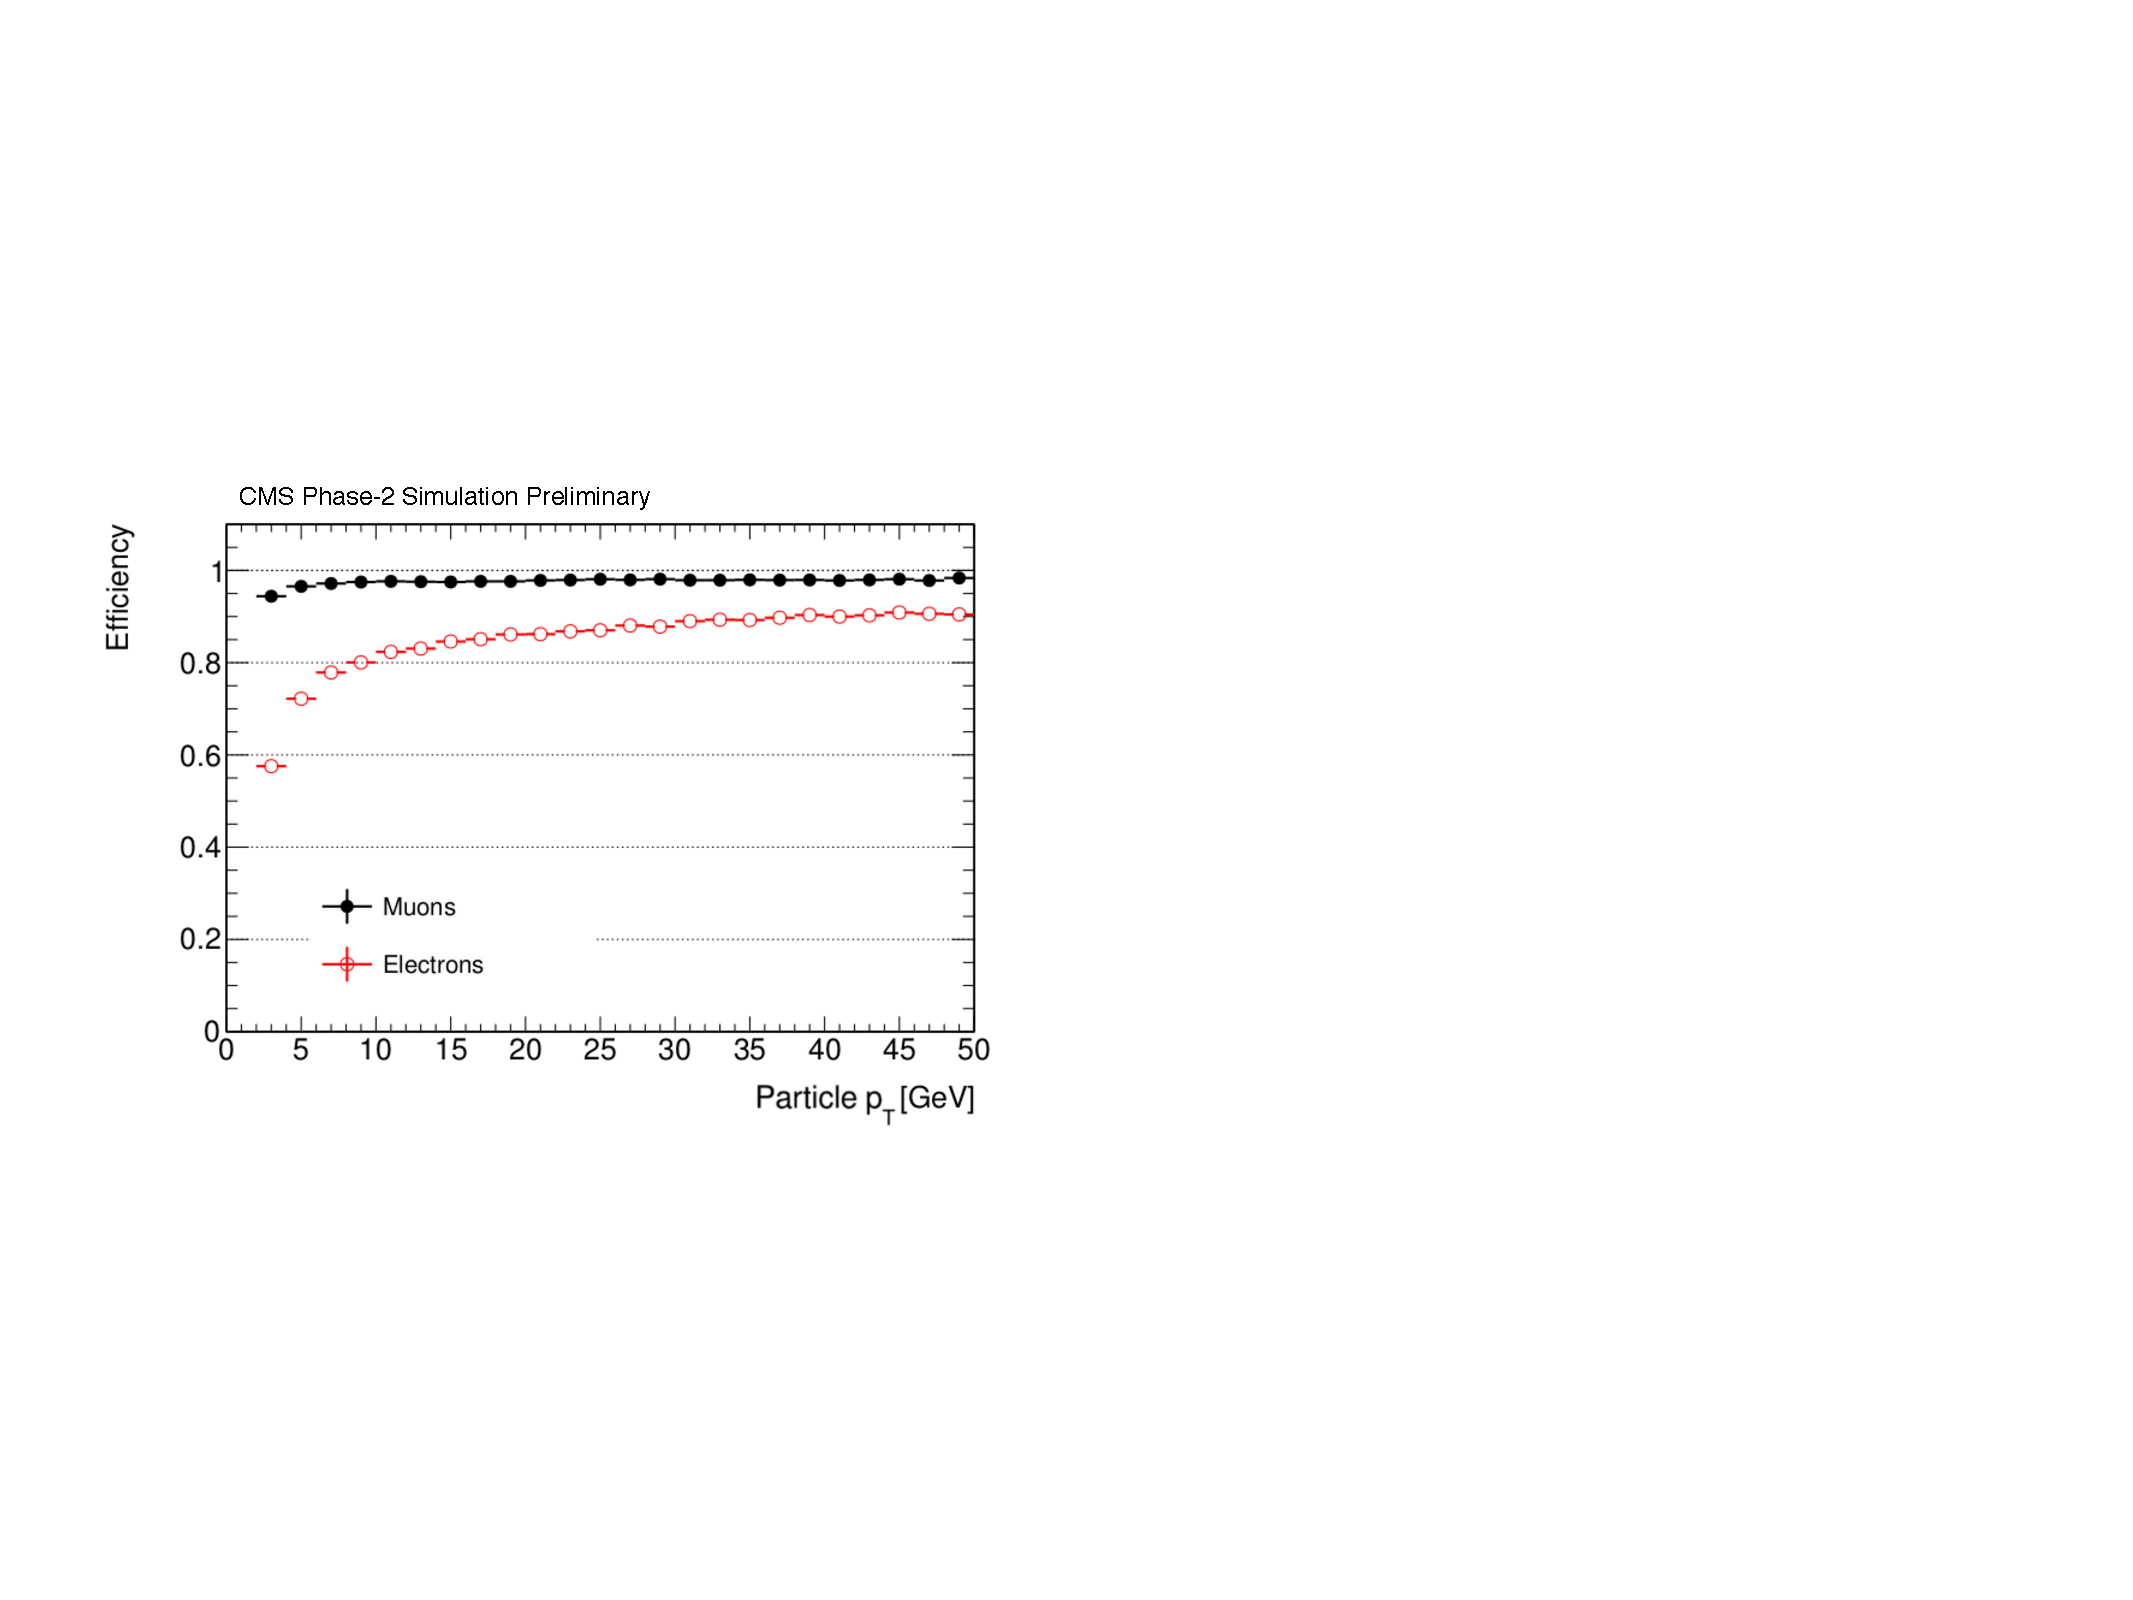
\includegraphics[width=0.47\textwidth]{figures/cmsupgrade/TDR-17-001_fig6_6_a.pdf} \hfill
  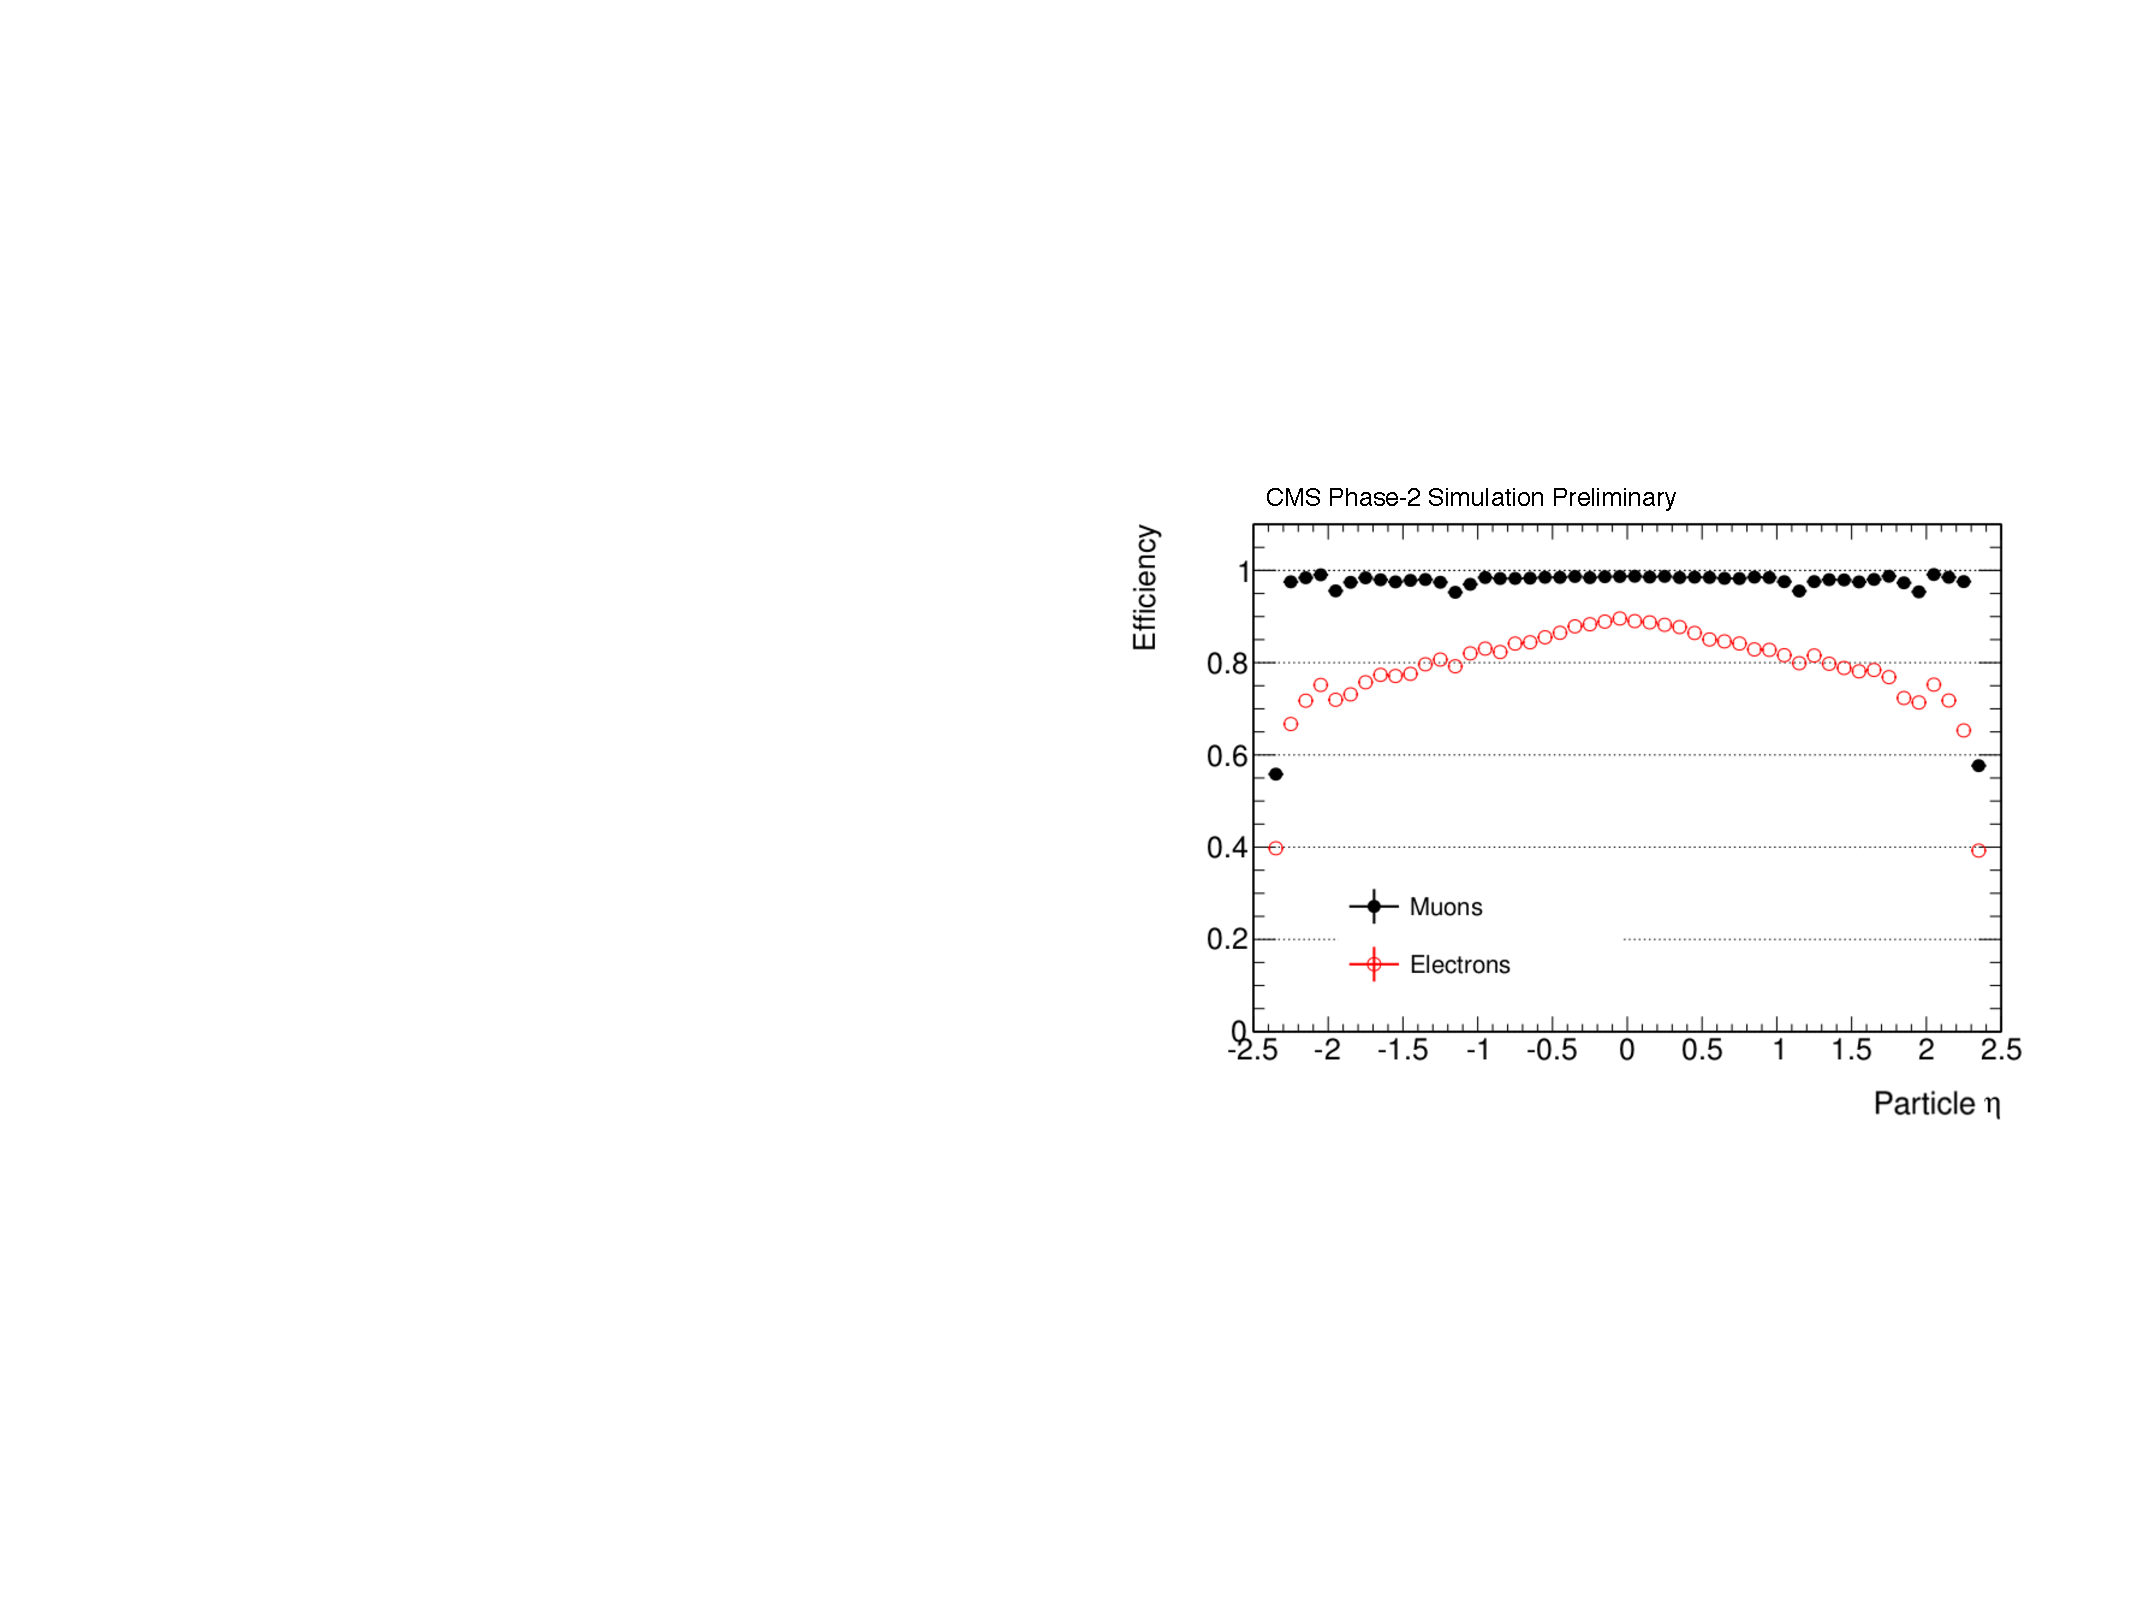
\includegraphics[width=0.47\textwidth]{figures/cmsupgrade/TDR-17-001_fig6_6_b.pdf}
  \caption{ Left: L1 tracking efficiency versus generated particle $p_T$ for $|\eta| < 2.4$.
	Right: L1 tracking efficiency versus $\eta$ for $p_T > 3$~GeV. Results for muons (electrons) are shown as filled black (open red) circles, and are produced with \ttbar events in a scenario with 200 pileup events on average. }
  \label{fig:cmsL1lepton}
\end{center}
\end{figure}

\begin{figure}[h!tbp]
\begin{center}
  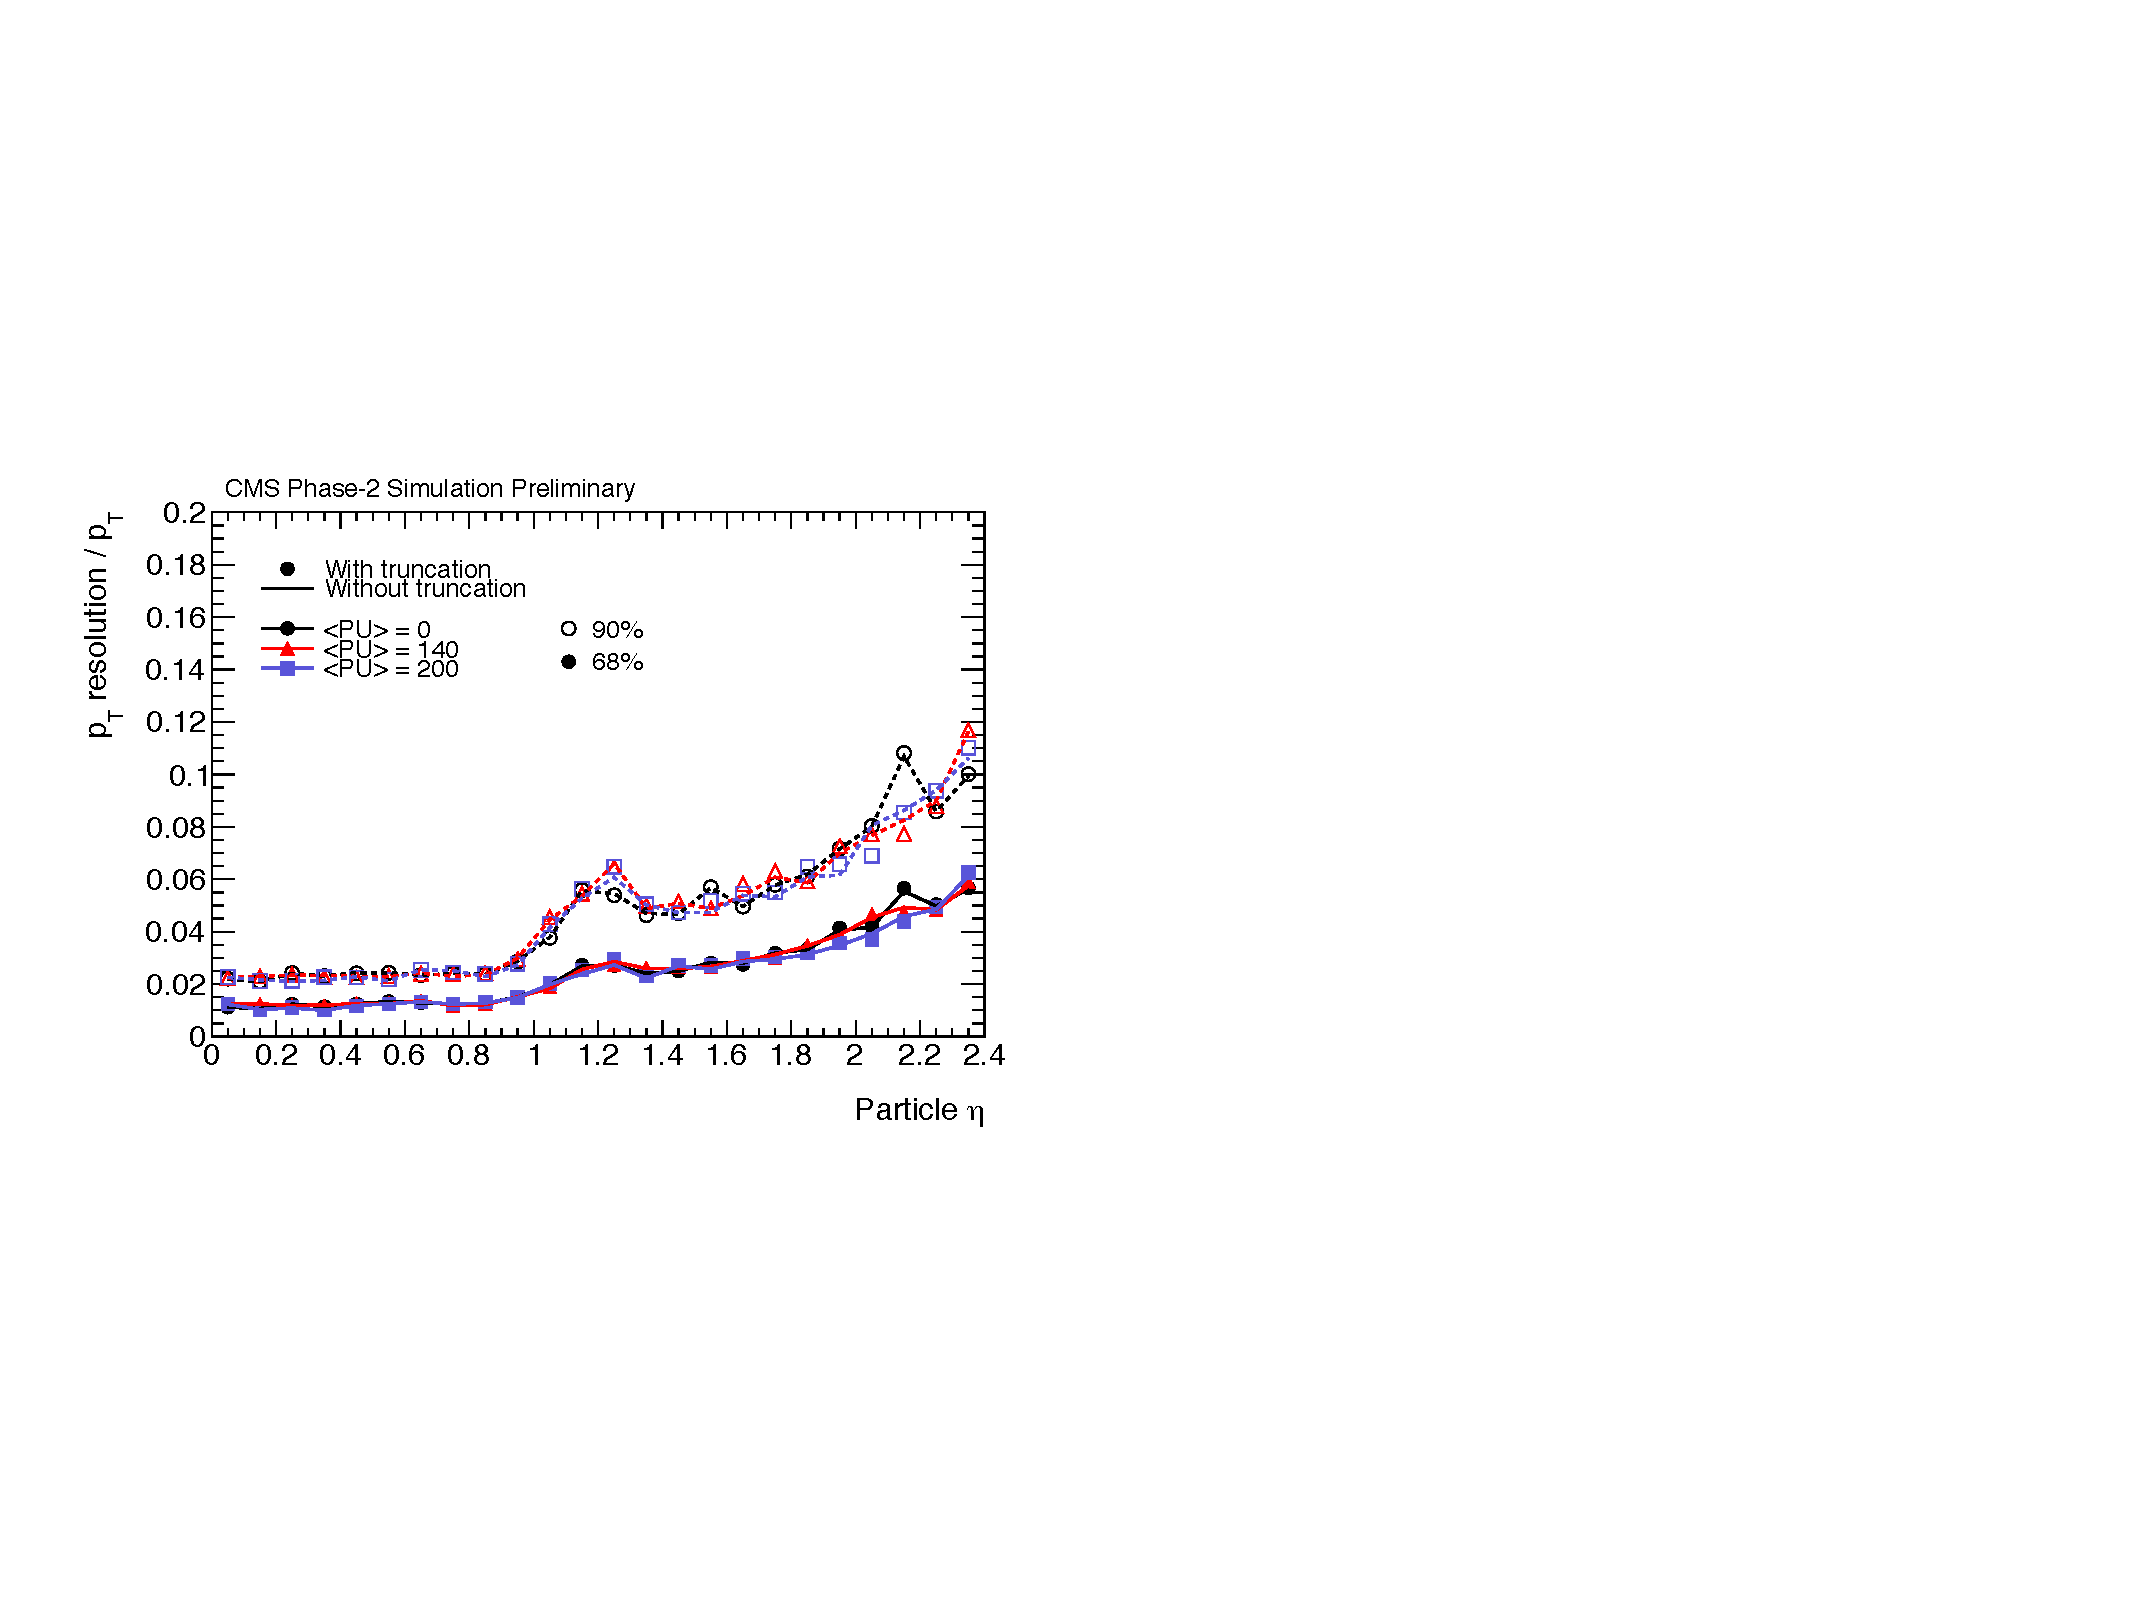
\includegraphics[width=0.47\textwidth]{figures/cmsupgrade/TDR-17-001_fig6_8_a.pdf} \hfill
  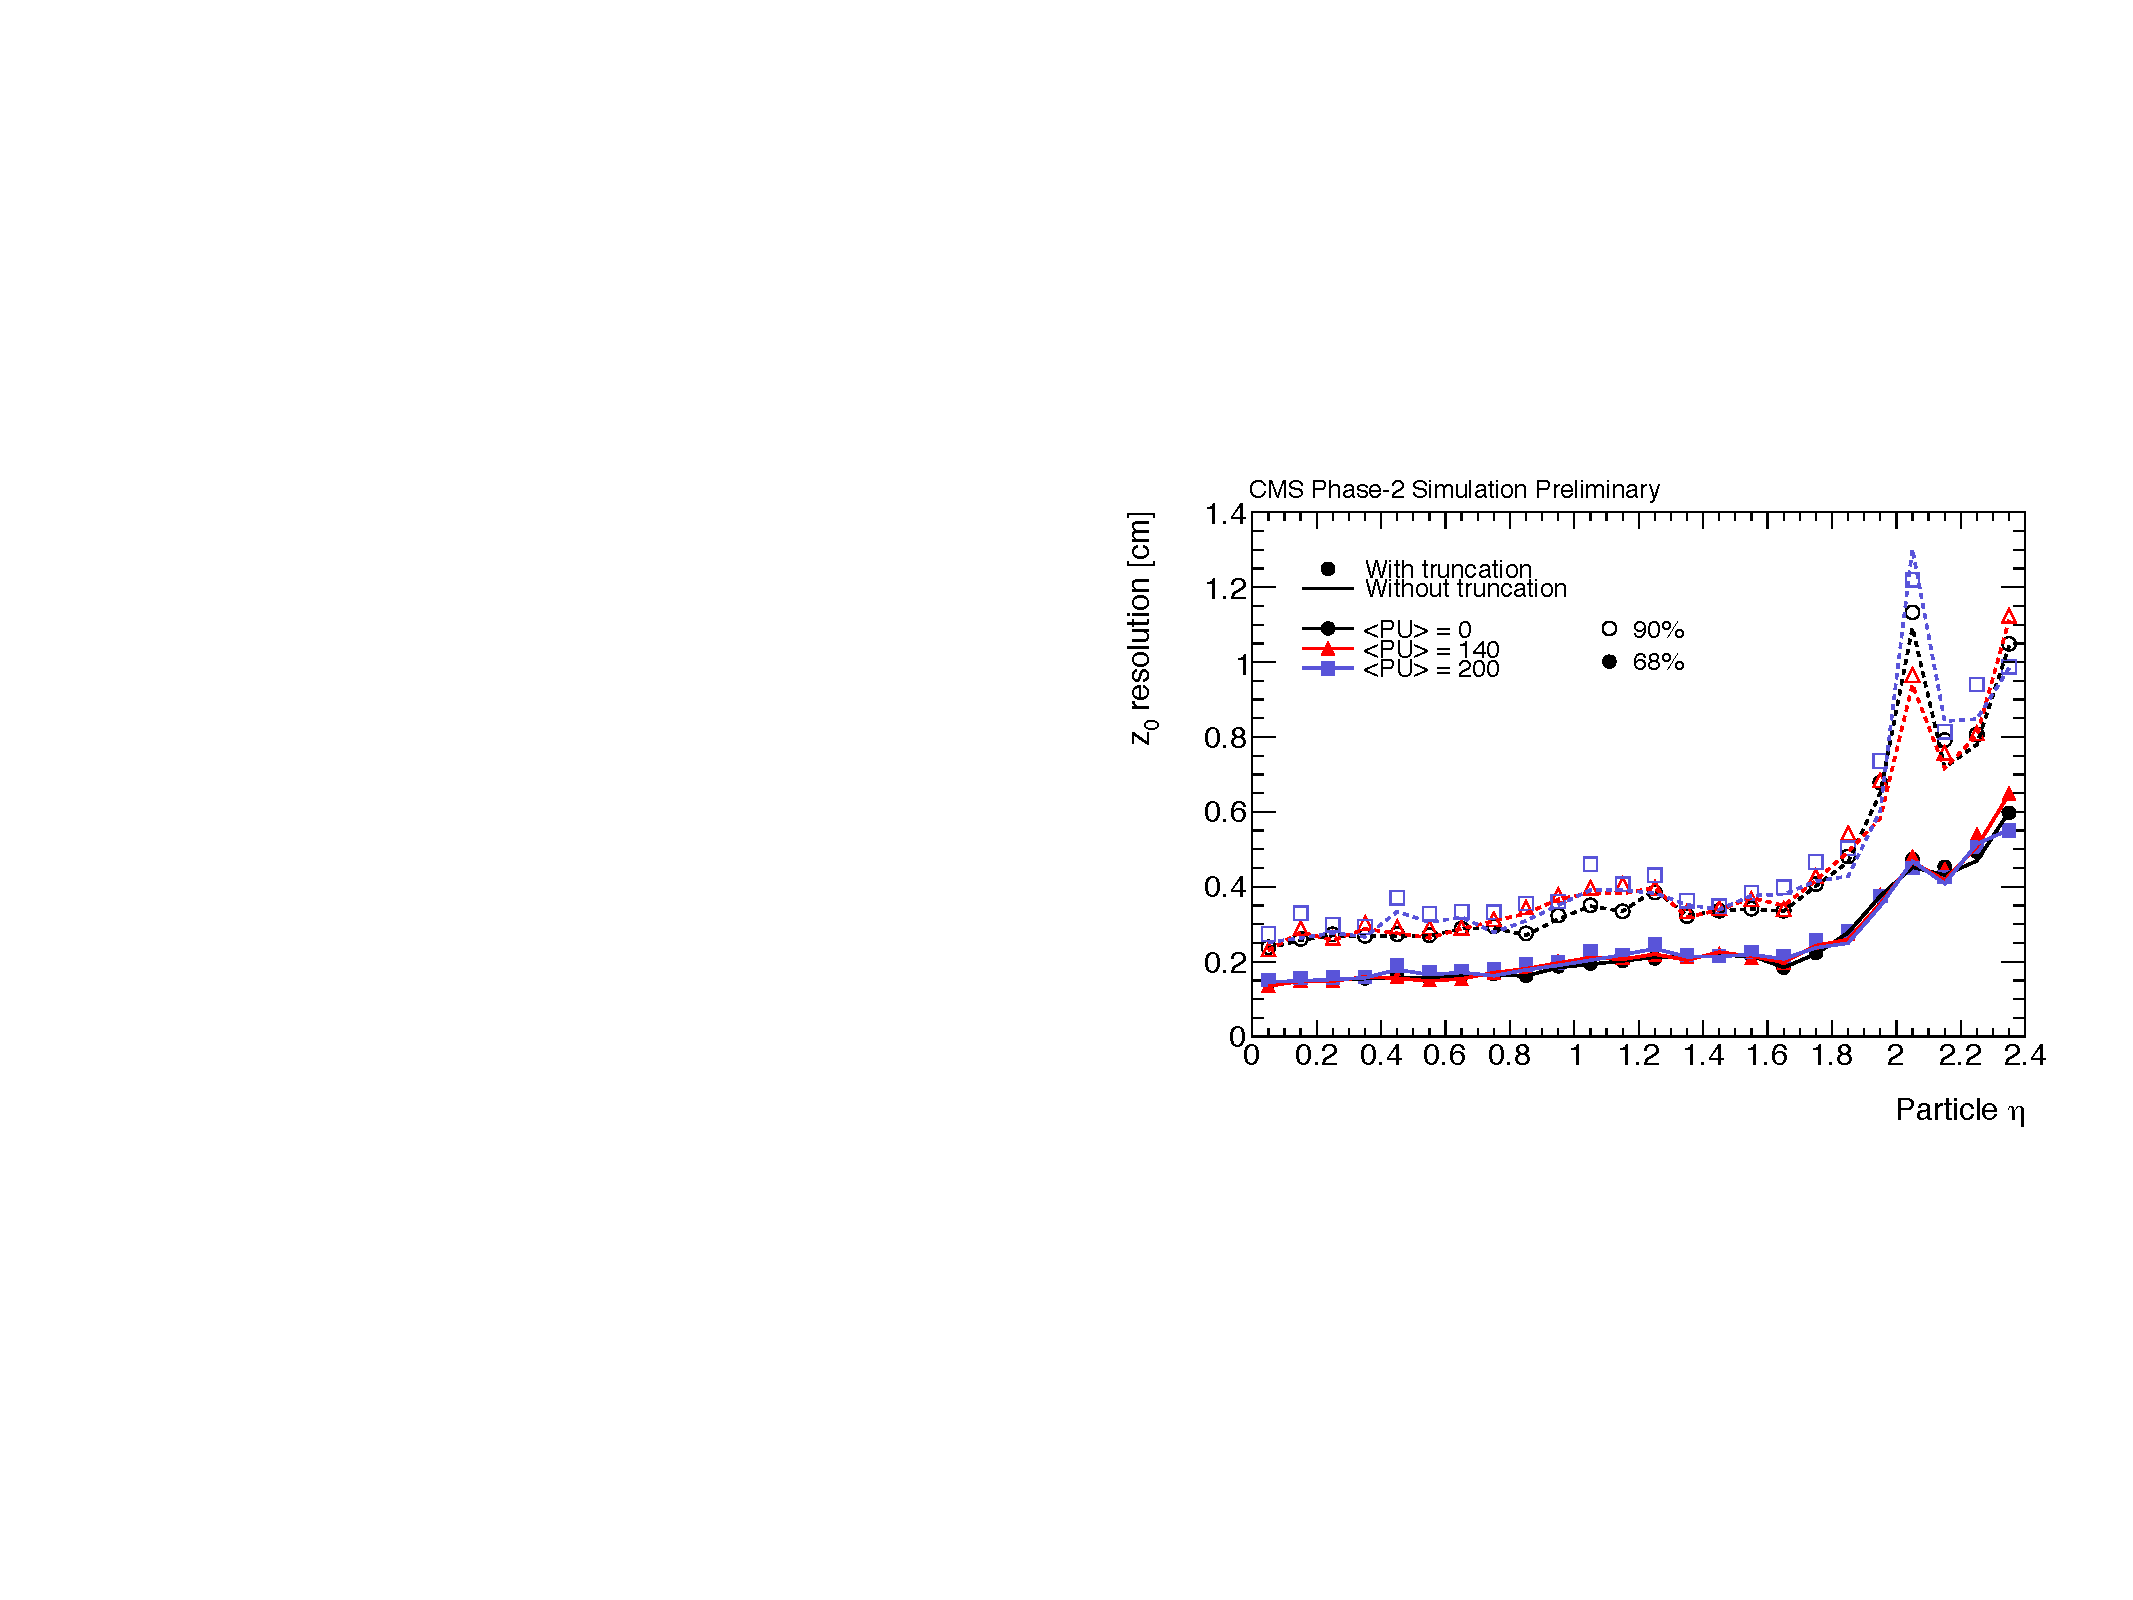
\includegraphics[width=0.47\textwidth]{figures/cmsupgrade/TDR-17-001_fig6_8_b.pdf}
  \caption{ Relative $p_T$ (left) and $z_0$ resolution versus pseudorapidity for muons in \ttbar events with zero (black dots), 140 (red triangles), and 200 (blue squares) pileup events on average. 
Results are shown for scenarios in which truncation effects are (markers) or are not (lines) considered in the emulation of L1 track processing. 
The resolutions correspond to intervals in the track parameter distributions that encompass $68\%$ (filled markers and solid lines) or $90\%$ (open markers and dashed lines) of all tracks with $p_T > 3$~GeV.  }
  \label{fig:cmsL1tracks}
\end{center}
\end{figure}

Preliminary results on the offline tracking performance over the full acceptance of the CMS tracker are excellent with further improvements expected as the detector design and simulation algorithms are optimized.
Figure~\ref{fig:cmstrackres} shows the resolution of the transverse momentum and the transverse impact parameter
for single muons with $p_T = 10$~GeV as a function of the pseudorapidity both with the current
detector and at the HL-LHC upgrade. The better hit resolution of the HL-LHC tracker and the reduction of the material budget result in a significantly improved
$p_T$ resolution. The transverse impact parameter resolution is also improved with respect to the current detector, ranging from below 10 mm in the central region to about 20 mm at the edge of the acceptance.

\begin{figure}[h!tbp]
\begin{center}
  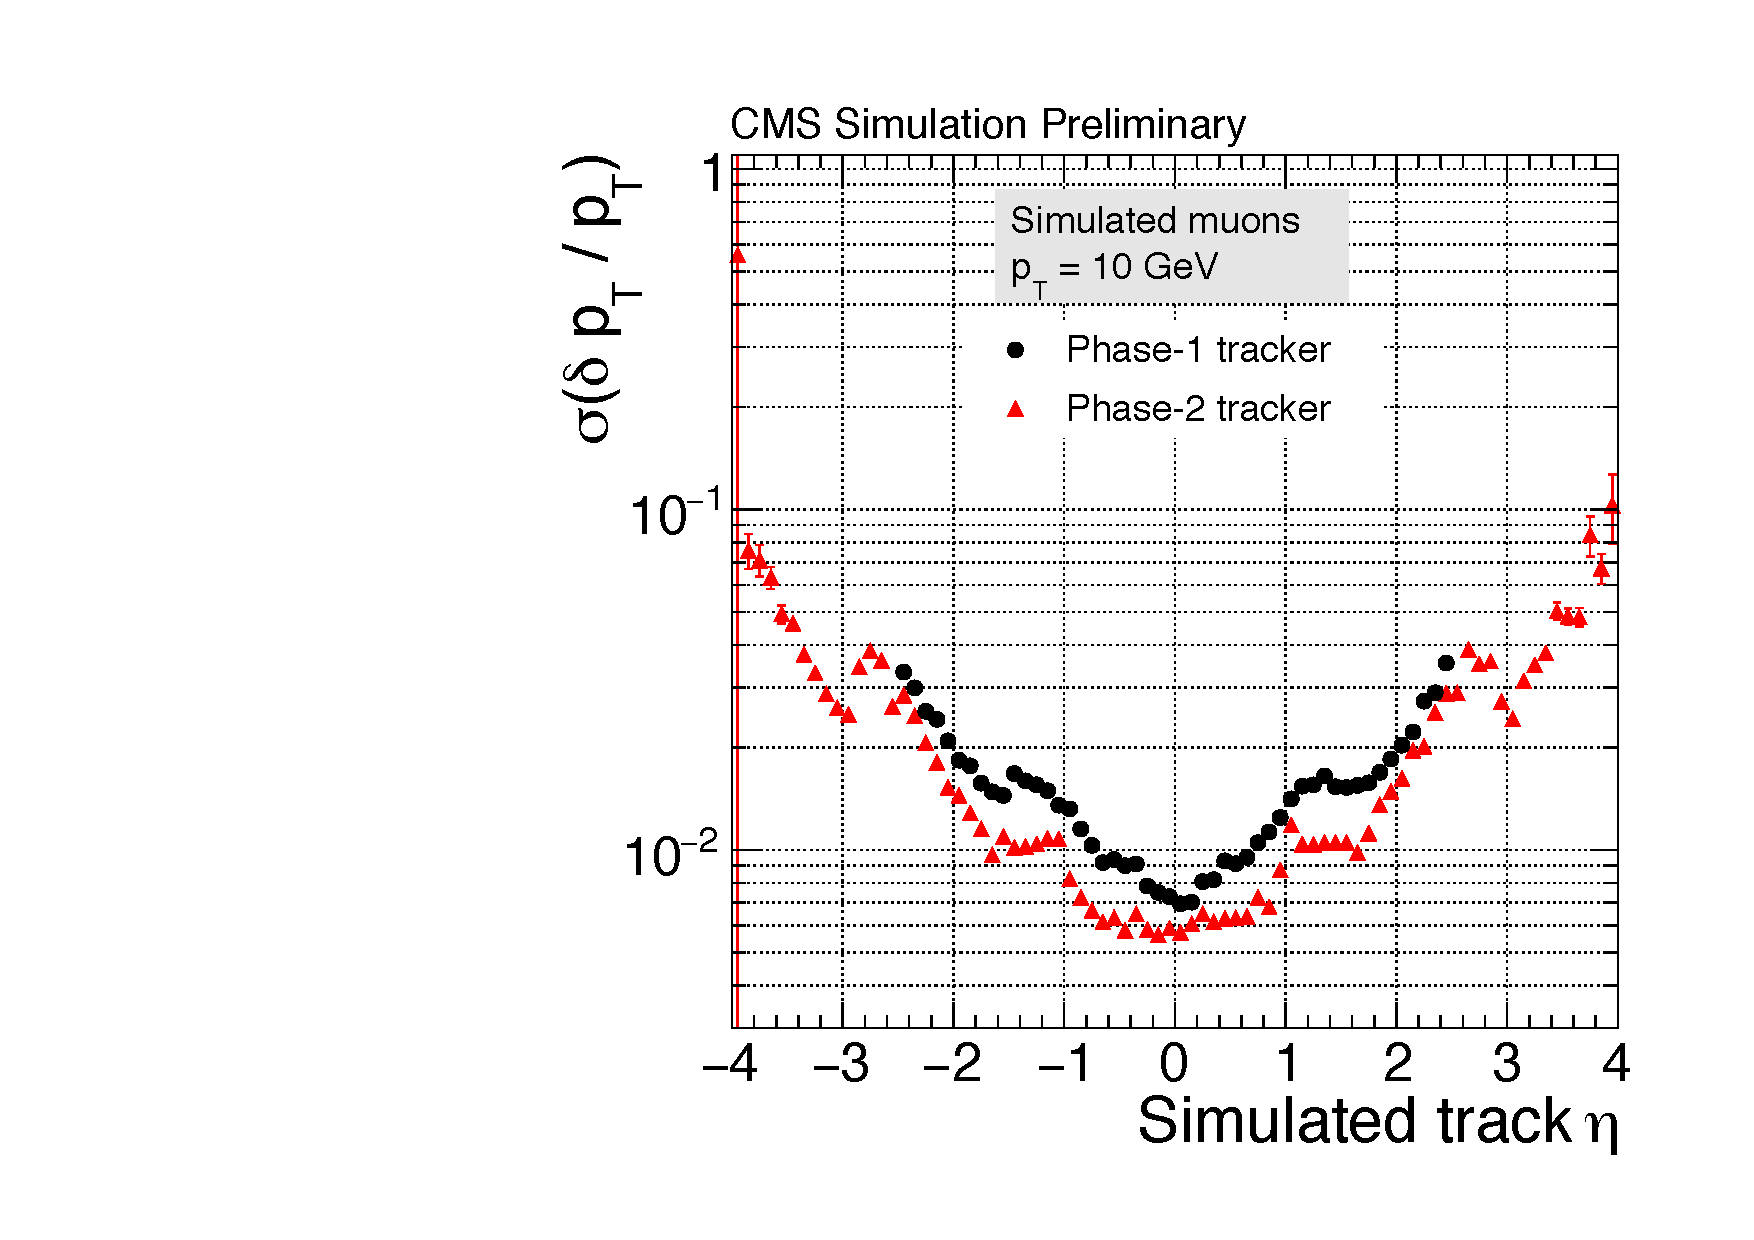
\includegraphics[width=0.47\textwidth]{figures/cmsupgrade/TDR-17-001_fig6_12_a_ptres_vs_eta_Sigma_vsPhase1.pdf} \hfill
  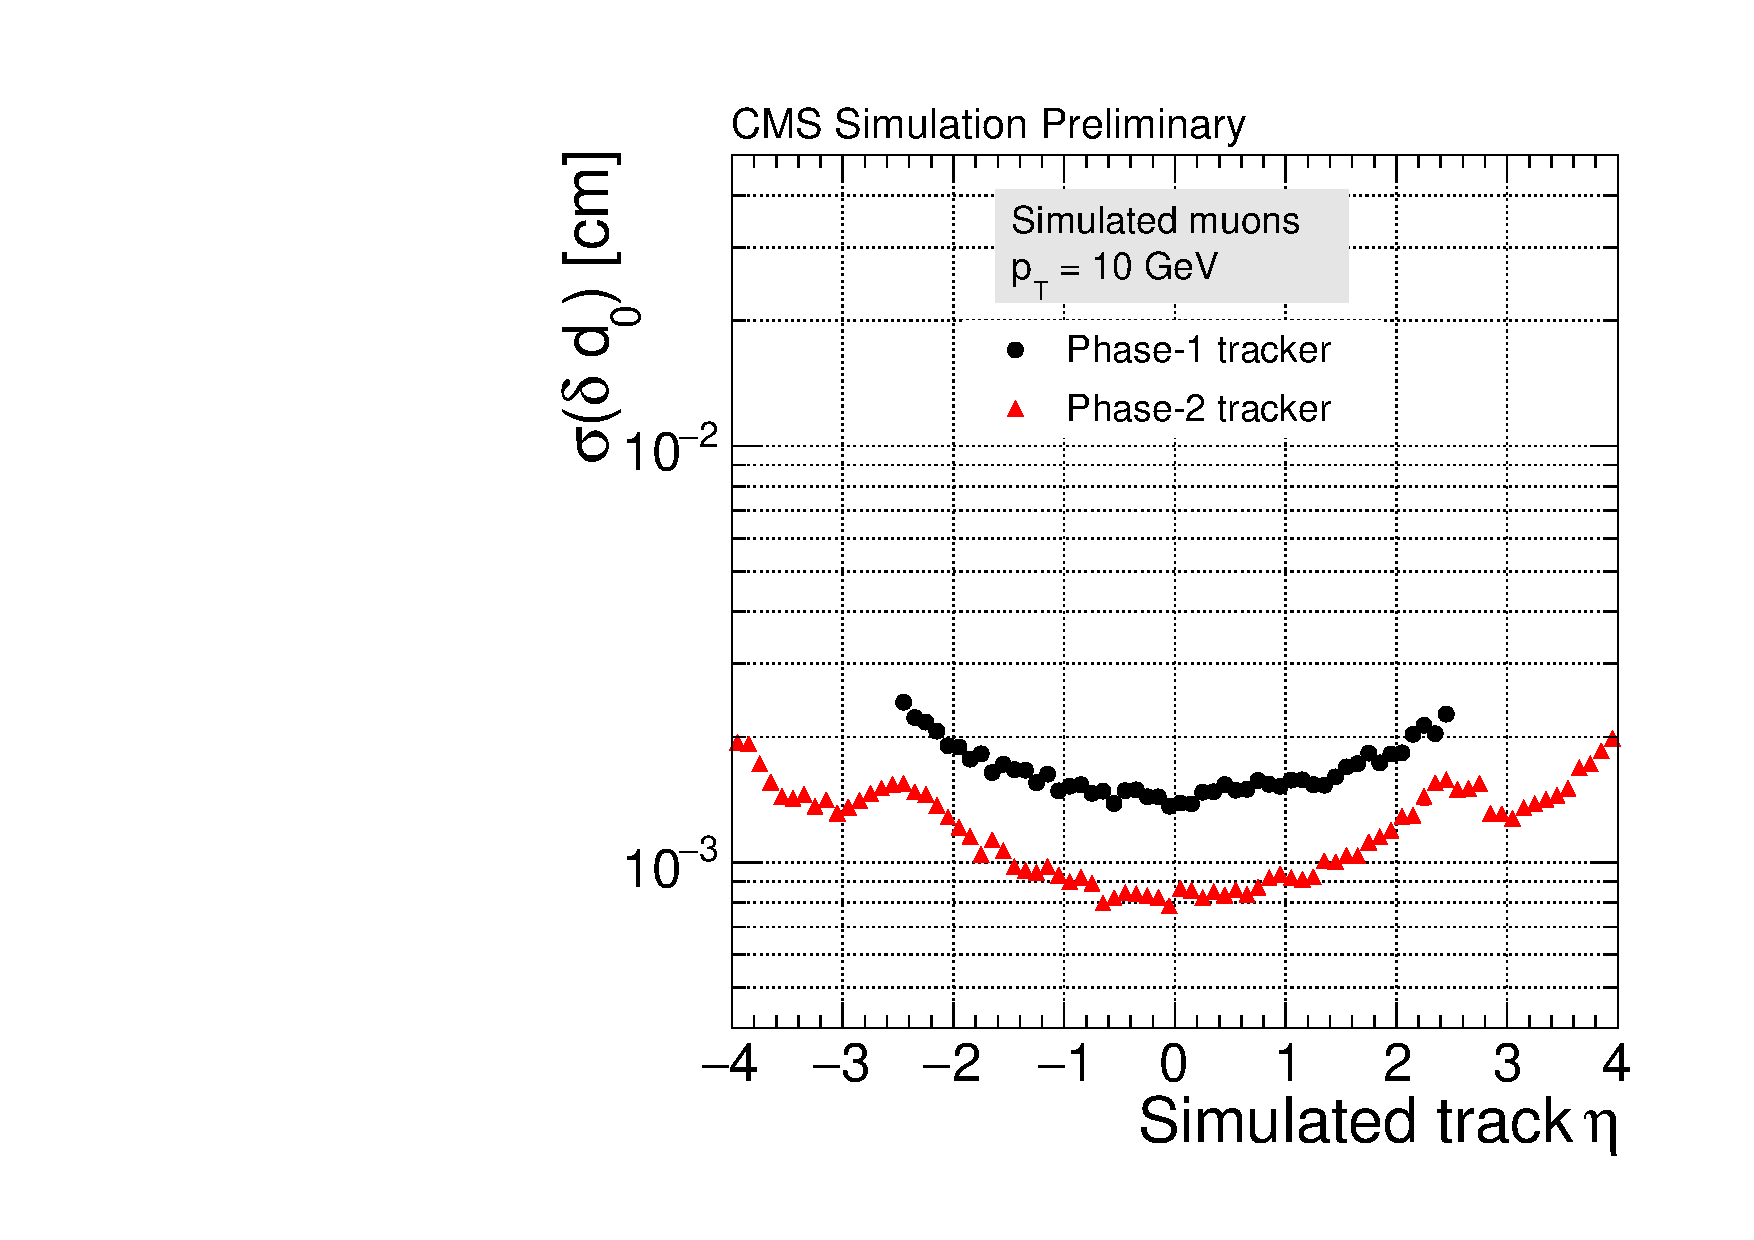
\includegraphics[width=0.47\textwidth]{figures/cmsupgrade/TDR-17-001_fig6_12_b_dxyres_vs_eta_Sigma_vsPhase1.pdf}
  \caption{ Relative resolution of the transverse momentum (left) and transverse impact parameter (right) as a function of the pseudorapidity for the current (black dots) and the upgraded (red triangles) CMS tracker, using single isolated muons with a transverse momentum of $10$~GeV. 
 }
  \label{fig:cmstrackres}
\end{center}
\end{figure}

For \ttbar~events, the efficiency to identify the primary vertex correctly is $\sim 95\%$ with 140 pileup events, and $\sim93\%$ with 200 pileup events. The vertex algorithm used is the
same as the one used in Run 2 for a pileup of about 35, therefore it is not yet optimized for vertex
reconstruction at very high pileup.
Figure~\ref{fig:cmsvertex} shows the resolution of the vertex position in the x, y, and z coordinates as a function of the number of tracks associated to the vertex. 
The vertex position resolution is almost independent of the amount of pileup in the event and the longitudinal resolution is only $50\%$
worse than the transverse one, as expected given the pixel dimensions of the inner tracker modules.

\begin{figure}[h!tbp]
\begin{center}
  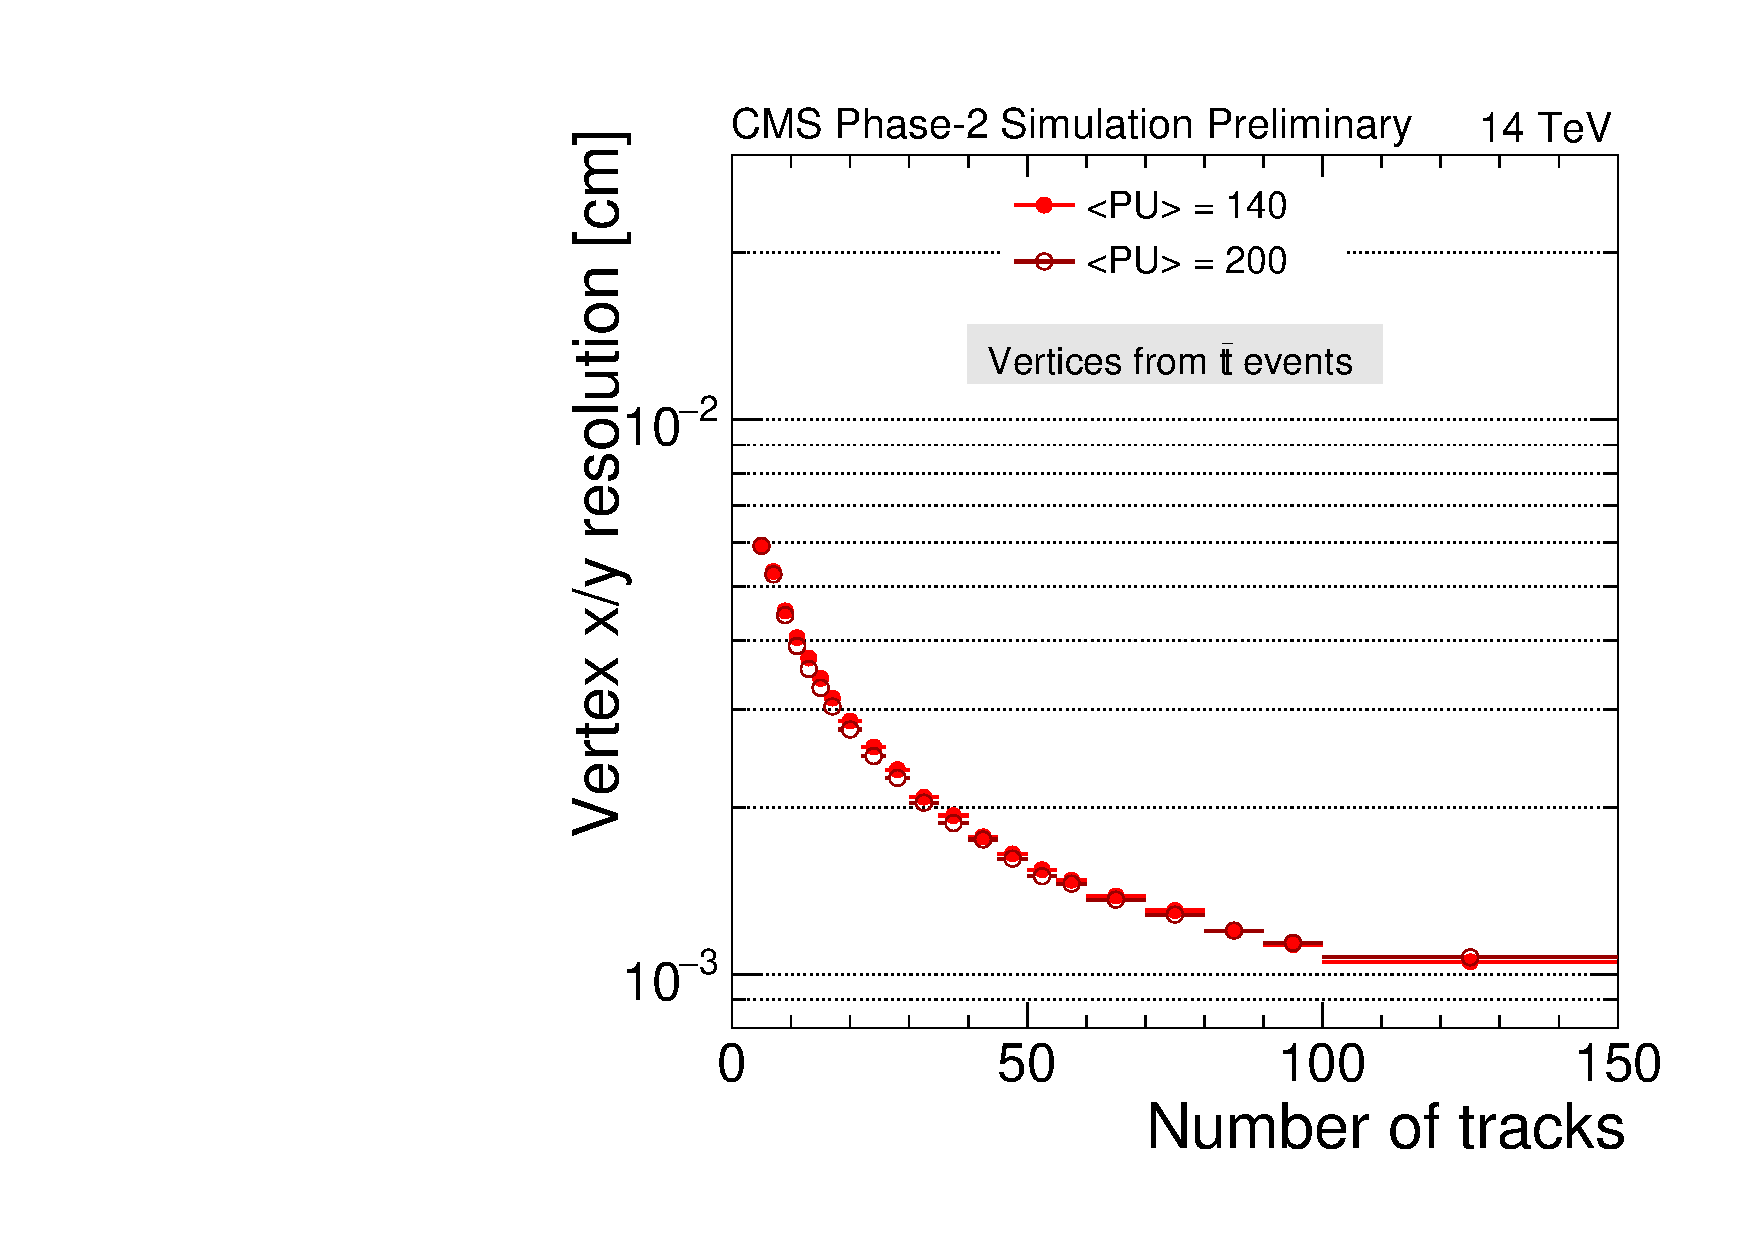
\includegraphics[width=0.47\textwidth]{figures/cmsupgrade/TDR-17-001_fig6_13_a_RecoAllAssoc2GenMatched_ResolX_vs_NumTracks_Sigma_PU.pdf} \hfill
  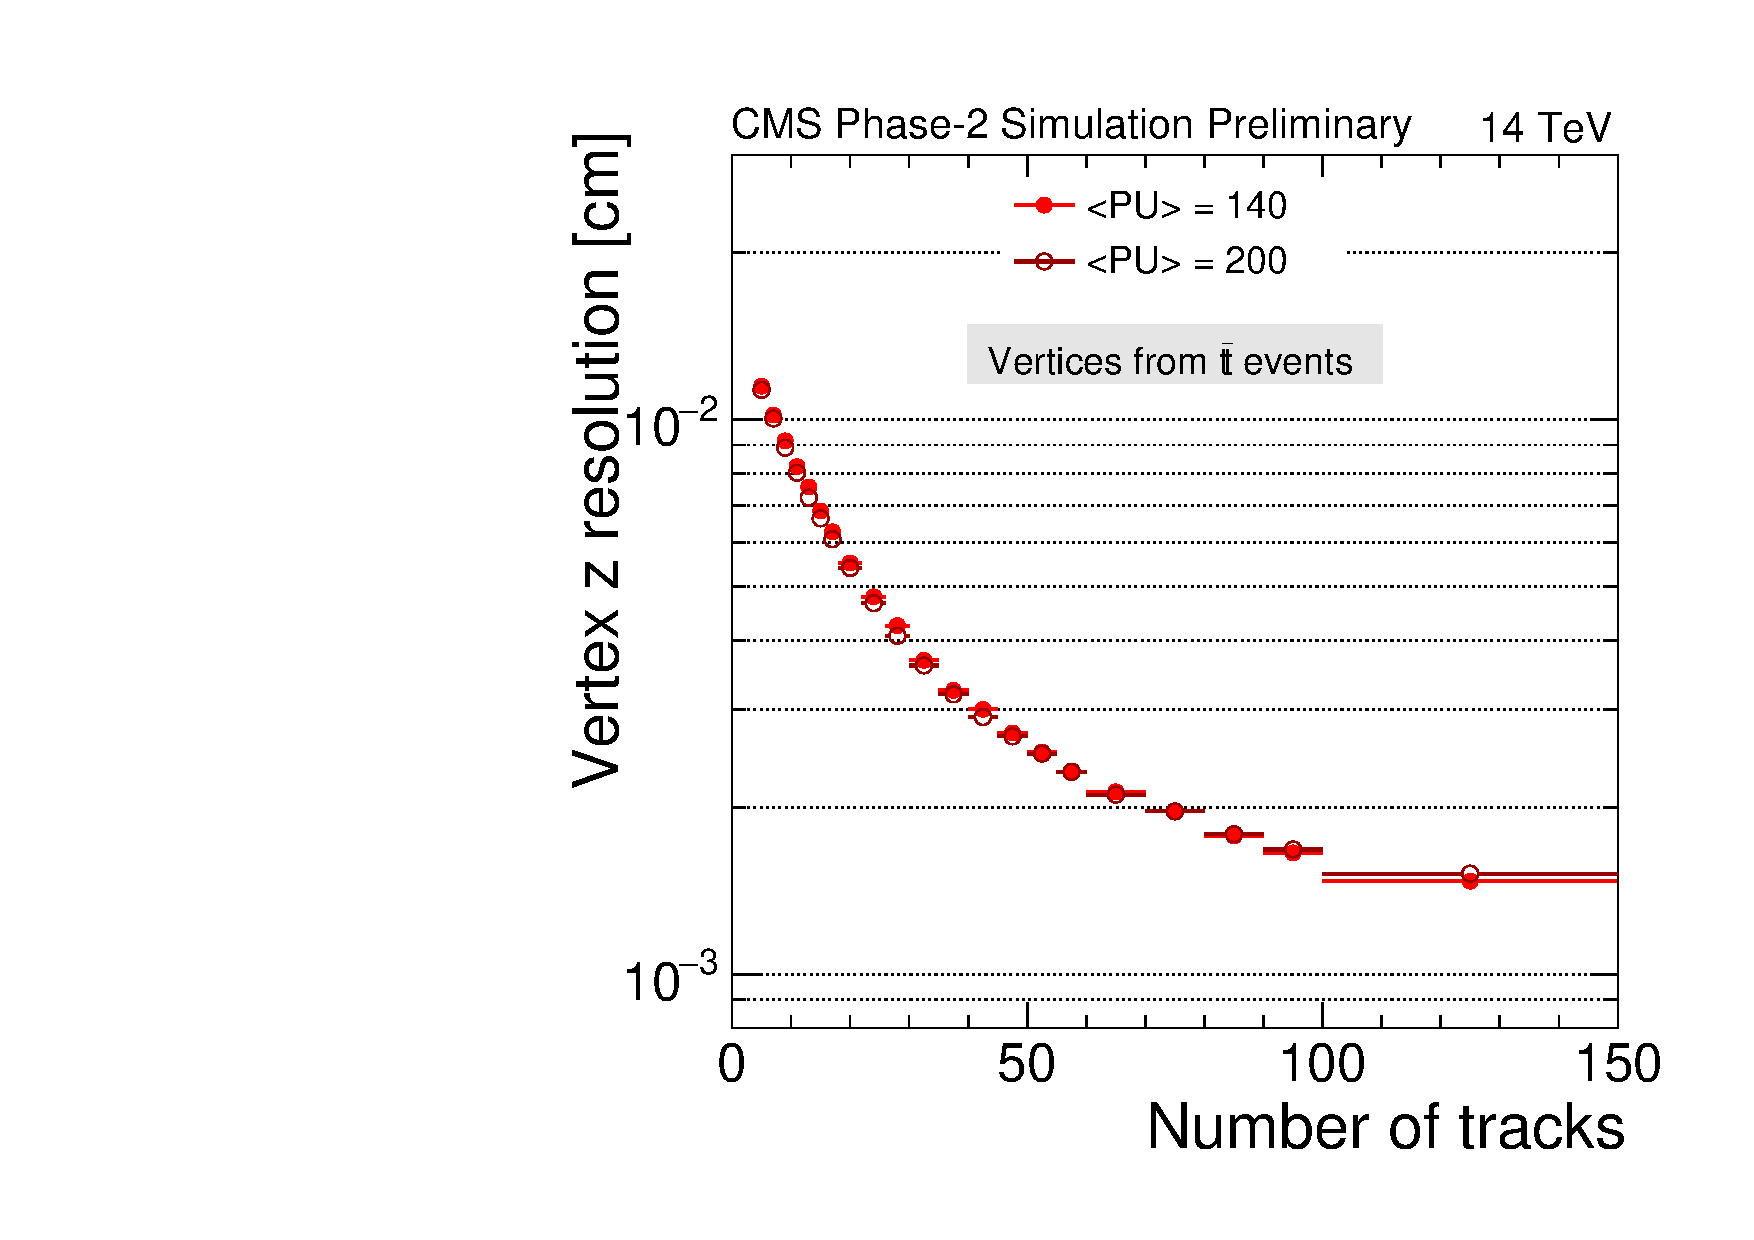
\includegraphics[width=0.47\textwidth]{figures/cmsupgrade/TDR-17-001_fig6_13_b_RecoAllAssoc2GenMatched_ResolZ_vs_NumTracks_Sigma_PU.pdf}
  \caption{Vertex position resolution in x and y (left) and z (right) as a function of the number of tracks associated to the vertex, for \ttbar events with 140 pileup events (full circles) and 200 pileup events (open circles). 
 }
  \label{fig:cmsvertex}
\end{center}
\end{figure}


Given that the CMS HLT tracking is based on the offline tracking code, a similar level of performance is expected.
Because of HLT time constraints, a parallelization of the algorithms is already under development and will be applied also in the HLT track reconstruction at HL-LHC.

\paragraph{ATLAS Performance}


\subsubsection{Leptons and Photon}

\paragraph{CMS Performance} 

At the L1 trigger level, the electron and photon trigger algorithms for HL-LHC will use information from the electromagnetic calorimeter as well as from the tracking detectors.
The algorithm should preserve the ability to reconstruct electromagnetic clusters with pT above a few GeV with high efficiency ($95\%$ or
greater above 10 GeV) as well as achieve high spatial resolution which should be as close as possible to the offline reconstruction.
Following the upgrade of both on-detector and off-detector electronics for the barrel calorimeters
in HL-LHC, the EB will provide energy measurements with a granularity of (0.0174, 0.0174)
in $(\eta, \phi)$, as opposed to the current input to the L1 trigger consisting of trigger towers
with a granularity of (0.087, 0.087). The much finer granularity and resulting improvement in position resolution of the electromagnetic trigger algorithms is critical in improving electron/
photon trigger efficiency and suppressing background at high pileup.
Figure~\ref{fig:cmsL1el} shows the comparison between the L1 EG (e-gamma) trigger algorithm in current (black)
based on trigger towers and the algorithm foreseen for HL-LHC (red), based on single crystal information.

\begin{figure}[hbtp]\begin{center}

\includegraphics[width=0.47\textwidth]{figures/placeholder.png}

\includegraphics[width=0.47\textwidth]{figures/placeholder.png}
\caption{ \textbf{CMS-TDR-017-002 Figure 9.19} Comparison between the Level-1 EG trigger algorithm in Phase-1 (black) and the
algorithm foreseen for Phase-2 (grey), based on single crystal information. Left: position resolution,
expressed in terms of DR with respect to the generated electron. Right: Level-1 EG
trigger efficiency as a function of the tranvserse momentum of the generated electron. An electron
gun sample, with flat pT spectrum between 8 and 100 GeV and an average pileup level of
200, was used for both measurements.
}
\label{fig:cmsL1el}
\end{center}
\end{figure}


The momentum resolution of the L1 muon trigger for muons coming from the primary vertex
will be greatly improved by adding information from the L1 track trigger. 
The L1 track trigger can also be directly combined with trigger primitives at the first stage of the muon
track finder electronics; this would mirror the offline reconstruction of ``Tracker Muons'' which
improve the efficiency for very low $p_T$ muons, especially in the barrel region.

Two classes of triggerable events from beyond-standard model physics require standalone
muon trigger capabilities not covered by the Track Trigger system, namely for displaced muons and heavy stable charged particles (HSCP). 
To trigger on both prompt and non-prompt muons effectively at L1, a standalone L1Muon generates two $p_T$ measurements for each muon, prompt and
non-prompt, which are matched with L1 tracks. 
If the track match is successful, the L1 track trigger $p_T$ is used and a
prompt candidate is formed. 
If the match is unsuccessful and the muon is not vetoed by L1 tracks, the
non-prompt L1Mu $p_T$ is used to form a displaced muon candidate.
Figure~\ref{fig:cmsL1mu} shows good performance for displaced muons with this method: reasonably high efficiency and a
trigger rate for single muon trigger around 10 kHz at HL-LHC conditions. Further improvements to the algorithm are underway to accomodate high pile-up conditions. 
The upgrade of the RPC system will allow the trigger and identification of slowly moving
particles by measuring their time of flight to each RPC station with a resolution of $O(1)$~ns. 
The speed of muon-like particles and the time (bunch crossing) of their
origin will be computed with a fast algorithm to be implemented in the L1 trigger for HL-LHC.
More details on the physics performance of displaced muon and HSCP searches are discussed in Section~\ref{sec:upgradesearch}.

\begin{figure}[h!tbp]
\begin{center}
  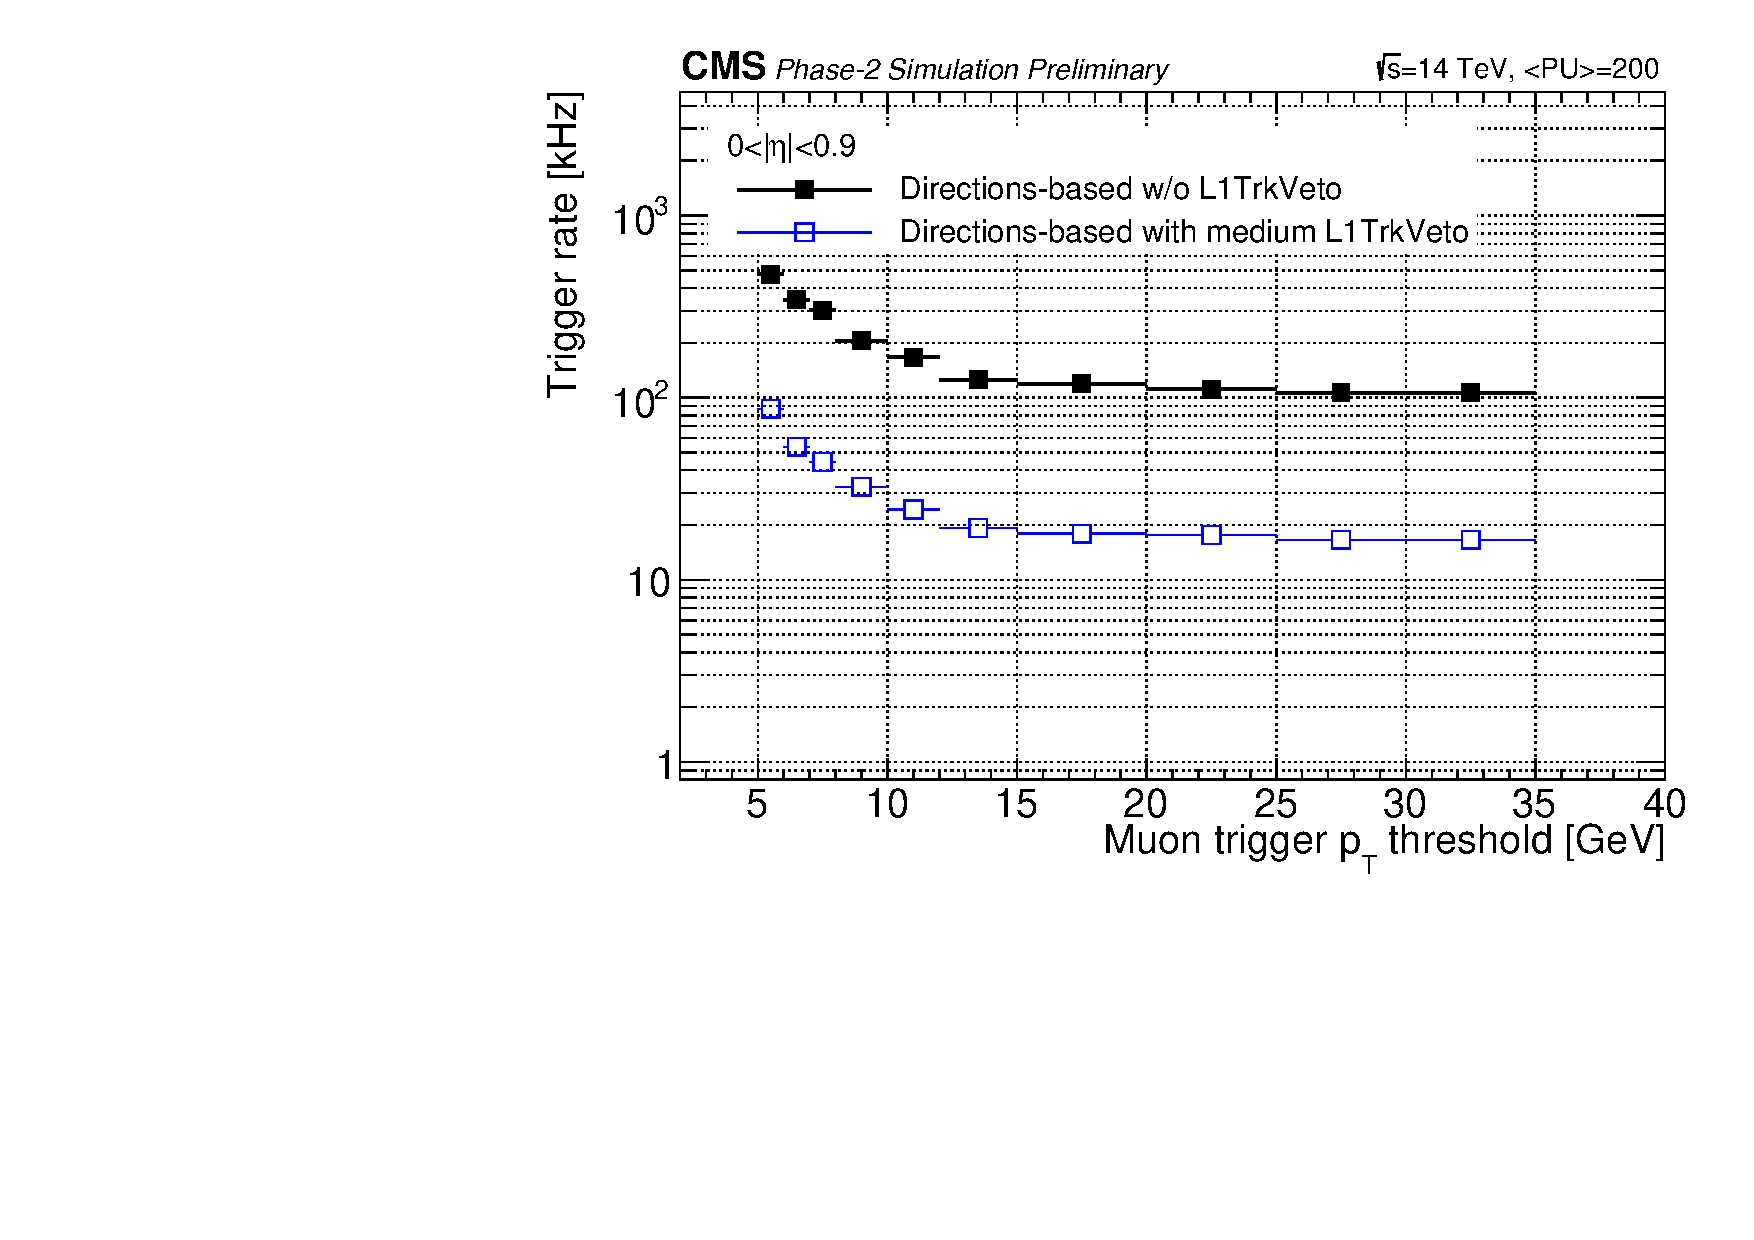
\includegraphics[width=0.47\textwidth]{figures/cmsupgrade/TDR-17-003_fig_7_11_a_Prompt_L1Mu_trigger_rate_pt__L1Mu__L1Mu2st__DisplacedL1MuDirectionBased_MB1_MB2_MB3_MB4_combined_eta0to0p9.pdf} \hfill
  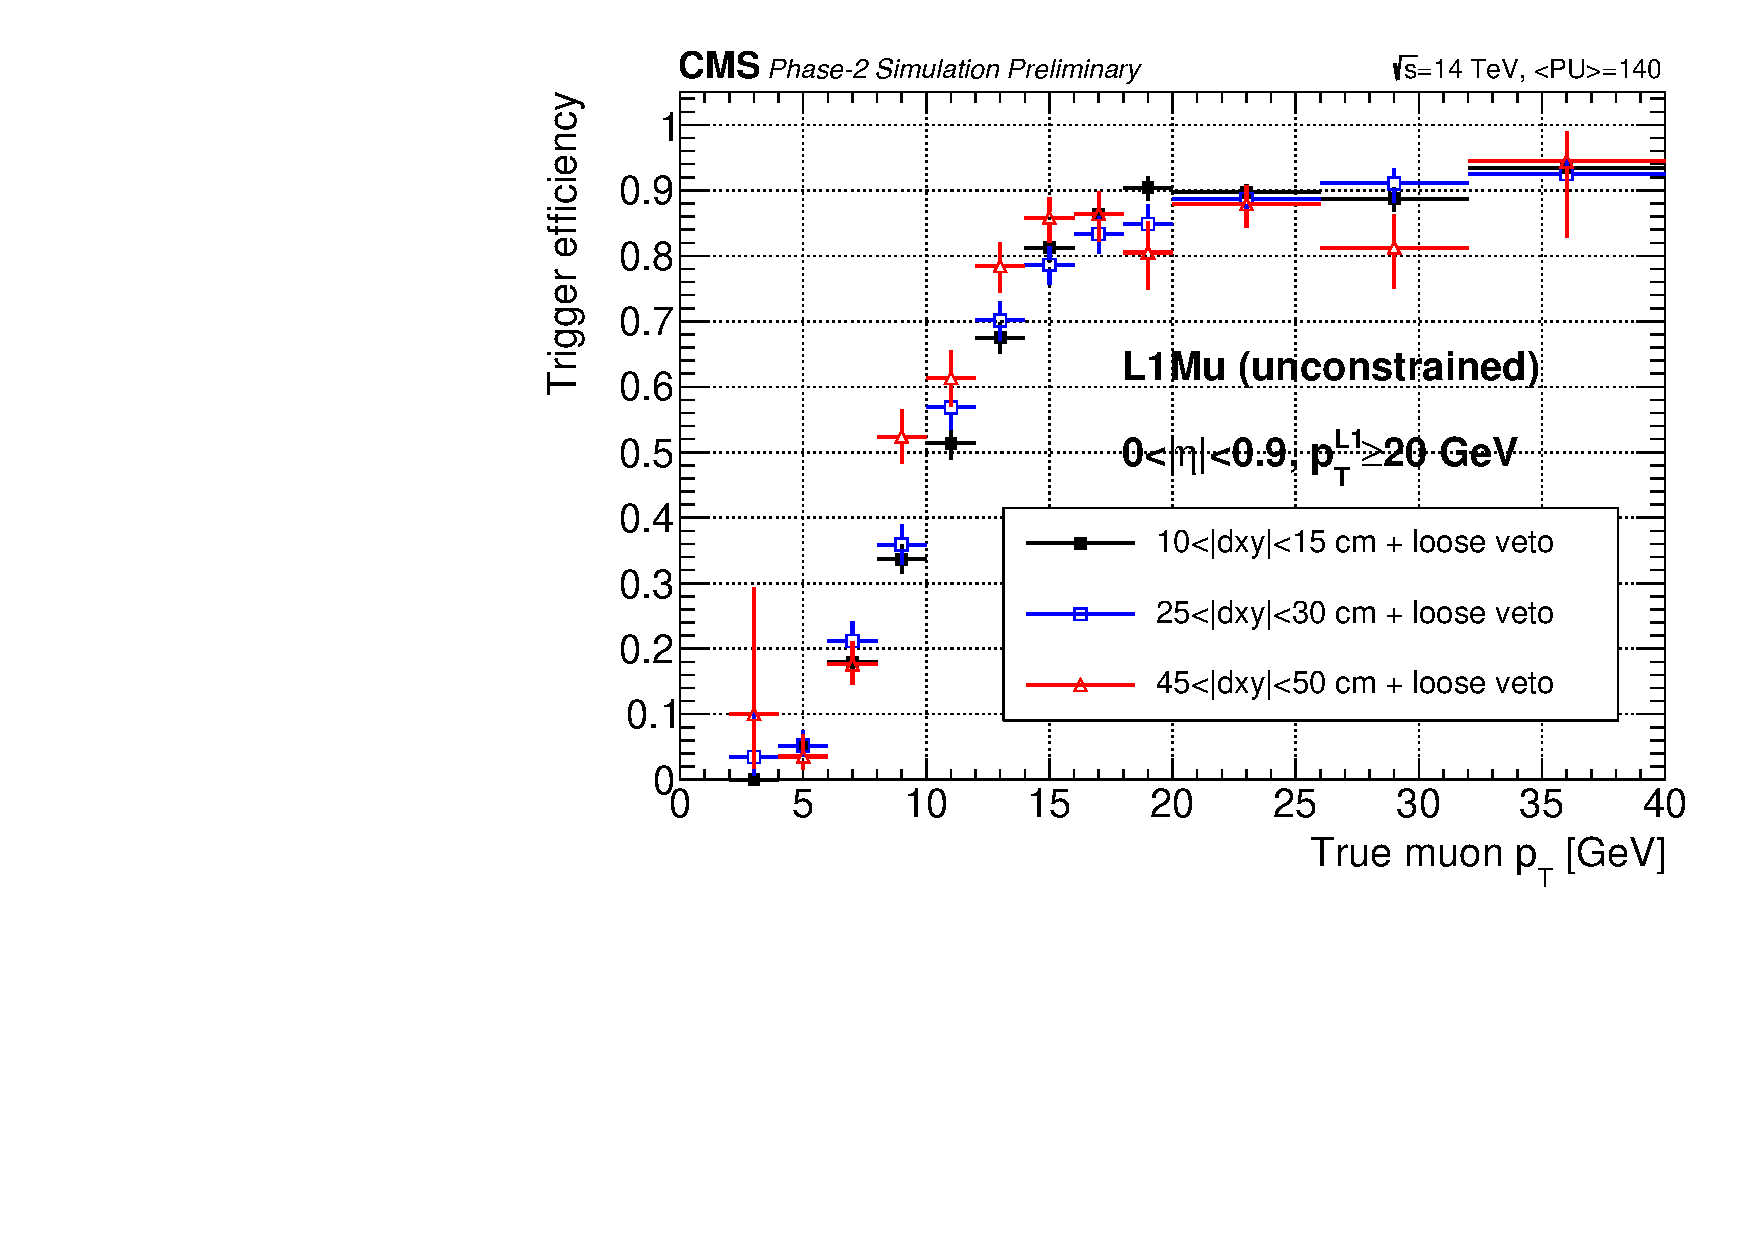
\includegraphics[width=0.47\textwidth]{figures/cmsupgrade/TDR-17-003_fig_7_11_b_L1MuonTDR2017Displaced_L1MuPt20_SimMuPt_DT1_DT2_DT3_DT4_combined_eta0to0p9_dxy5to50_looseVeto.pdf}
  \caption{ L1 Muon trigger rate (left) and efficiency (right) versus muon $p_T$ threshold for the barrel displaced muon algorithm. 
 }
  \label{fig:cmsL1mu}
\end{center}
\end{figure}


\paragraph{ATLAS Performance}


\subsubsection{Jets and Missing Energy}

\paragraph{CMS Performance} 

(TBA with HGCAL TDR approval) 

\paragraph{ATLAS Performance}



\subsection{Upgrade Projection: LLP Searches} \label{sec:upgradesearch}

Searches for long-lived particles are well motivated by various classes of extensions of the Standard Model. 
Often, the cross section for such processes is expected to be very small. The HL-LHC will allow for the collection of much larger data sets needed to reach better sensitivity. 
The prospects are further strengthened with detector and trigger upgrades. 
This section discusses these potential improvements, and presents sensitvity projections on a number of benchmark LLP models with the aforementioned upgrades at HL-LHC. 

\subsubsection{Heavy Stable Charged Particles}

A number of new physics scenarios give rise to heavy stable charged particles (HSCP) with long lifetimes that move slowly through the detector, heavily
ionizing the sensor material as they pass through. 
In Split SUSY models, the supersymmetric particles stau ($\tilde{\tau}$) and gluino ( $\tilde{g}$) can have such characteristic signatures.

\paragraph{Sensitivity projection with tracker upgrade} 

Depending on their mass and charge of the new particles, HSCPs leave anomalously high energy loss through ionization ($dE/dx$) in the silicon sensors with respect to the typical energy loss for SM particles, as can be seen in Figure~\ref{fig:cmsupgrade_hscp} (left).
At the CMS experiment, the current strip tracker features analogue readout, and the pixel detector featured analogue
readout at Phase-0 and features digital readout at Phase-1, allowing for excellent $dE/dx$ measurements.

At the HL-LHC, the upgraded CMS inner pixel detector will continue providing $dE/dx$ measurements, enabled
by its Time over Threshold readout, while the Outer Tracker cannot provide such information, given that the readout is binary. 
To increase the sensitivity for signatures with anomalously high ionization loss, a second, programmable, threshold has been implemented in the Short
Strip ASICs of the pixel-strip (PS) modules of the Outer Tracker, and a dedicated readout bit signals if a
hit is above this second threshold.  

Searches for HSCPs can thus be performed by measuring the energy loss in the inner pixel detector and by
discriminating HSCPs from minimum ionizing particles based on the ``HIP flag" in the Outer
Tracker. The threshold of the minimum ionization needed to set the HIP flag is an adjustable
parameter in the PS modules. A threshold corresponding to the charge per unit length of 1.4
MIPs, resulting from preliminary optimization studies, is used in the simulation, and the gain
in sensitivity obtained by using the HIP flag is studied.

An estimator of the degree of compatibility of the track with the MIP hypothesis is defined
to separate candidate HSCPs from tracks from SM background sources. The high resolution
$dE/dx$ measurements provided by the inner pixel modules are used for the computation of
the $dE/dx$ discriminator. 
The tracks in background events have a low number of high threshold clusters with HIP flag, compared to those observed for
tracks in HSCP signal events and slow moving protons and kaons in minimum bias events.

Figure~\ref{fig:cmsupgrade_hscp} (right) shows the performance of the discriminator by evaluating the signal versus background
efficiency curves to identify tracks from signal events and reject those originating from backgrounds. The performance curves are evaluated for two different strategies for
the discriminator: the dE/dx discriminator, which relies solely on the inner pixel modules
(``$dE/dx$-only"), ignoring the HIP flags, and a recomputed discriminator which includes the
HIP flags from the Outer Tracker PS modules (``$dE/dx$+HIP flag"). The signal versus background
efficiency performance curves demonstrate that for a background efficiency
of $10^{-6}$, analogous to the current analysis performance, the $dE/dx+$HIP-based discriminator
leads to an expected signal efficiency of $40\%$, around 4 to 8 times better than the $dE/dx$-only
discriminator. In the $dE/dx$-only scenario, the efficiency for the HSCP signal is about 8 times
smaller than that obtained in current data. The inclusion of the HIP flag for the PS modules of the Outer Tracker restores much of the efficiency, so that the
same sensitivity as in Phase-1 will be realized with about four times the luminosity of Phase-1.
The Phase-1 sensitivity will be surpassed with the full expected integrated luminosity of the
HL-LHC. This study demonstrates the critical impact of the HIP flag in restoring the sensitivity
of the CMS tracker for searches for highly ionizing particles.

\begin{figure}[h!tbp]
\begin{center}
  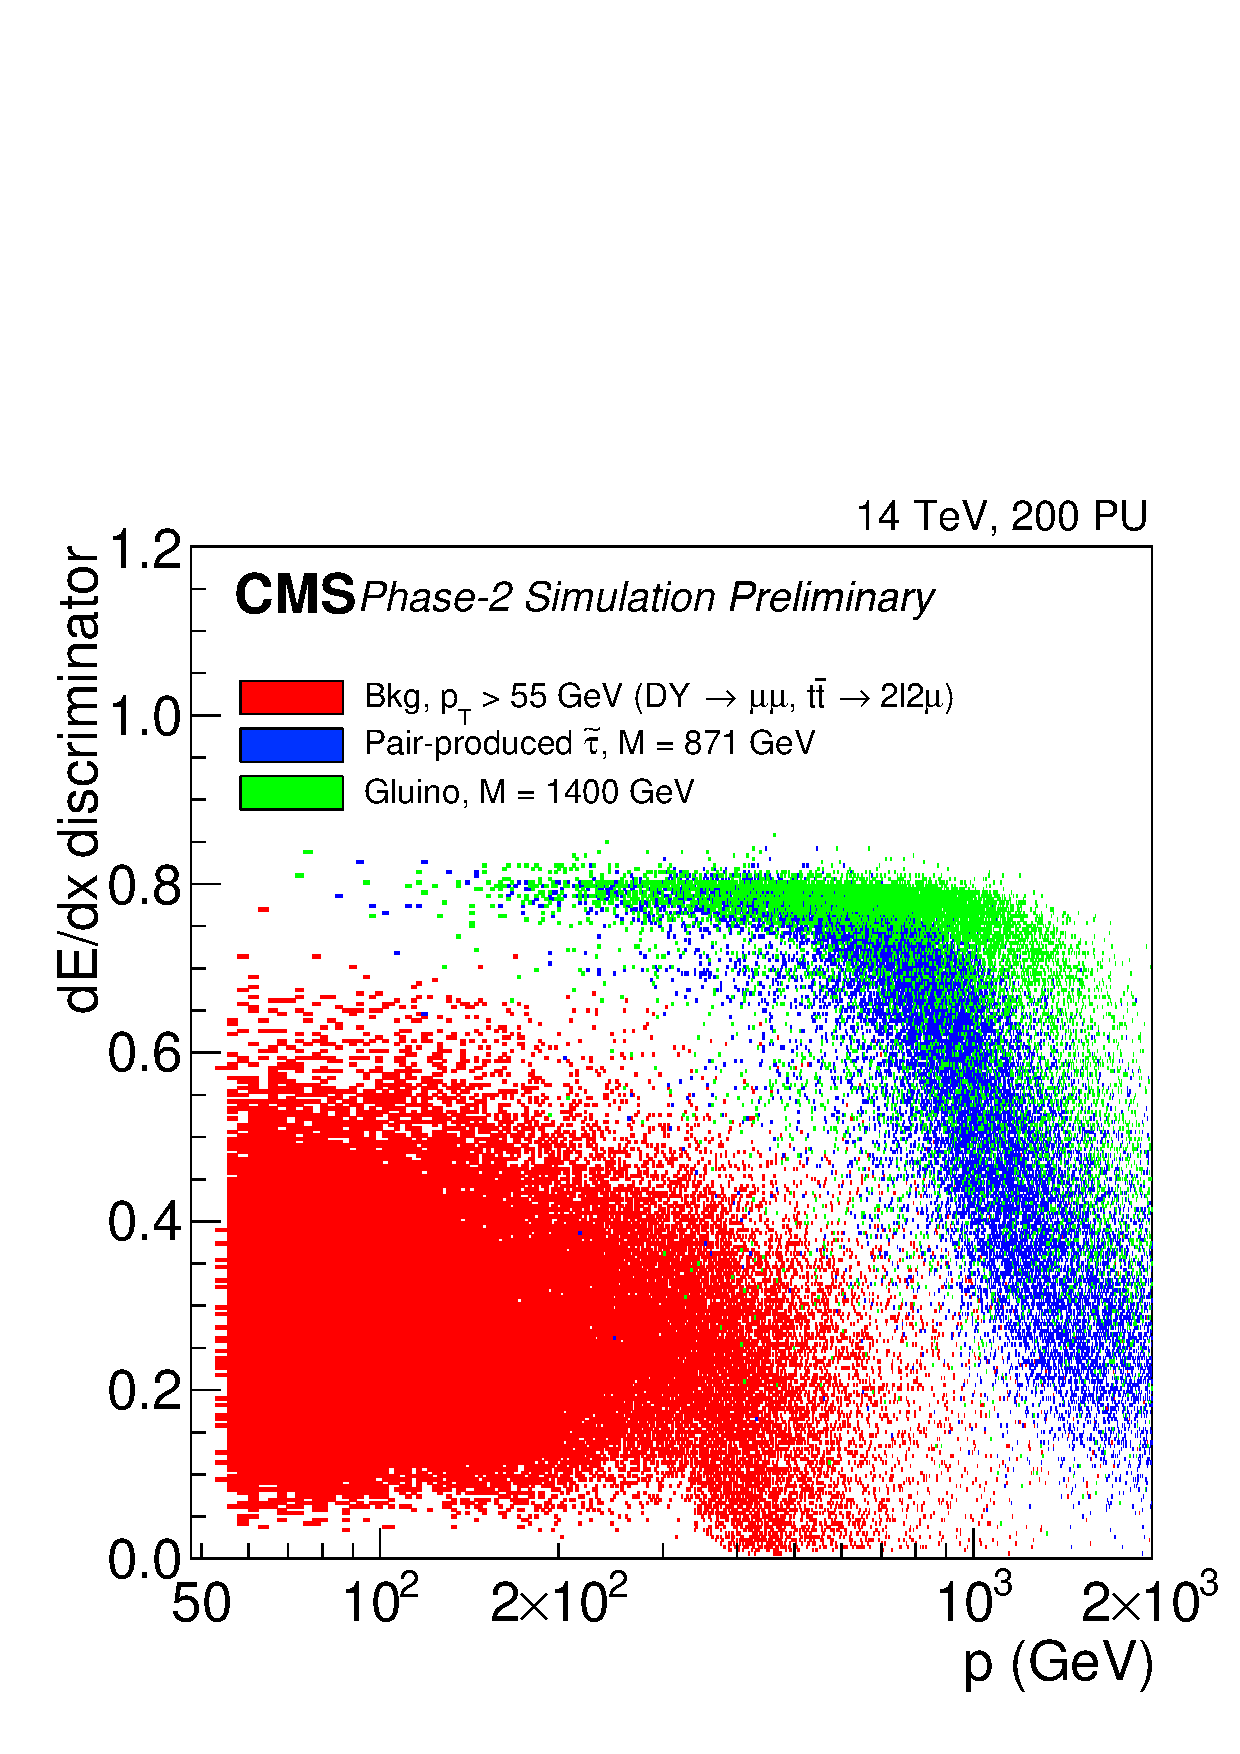
\includegraphics[width=0.47\textwidth]{figures/HSCP/TDR-17-001_fig6_26_a_HSCP_SpecialPlot_v2.pdf} \hfill
  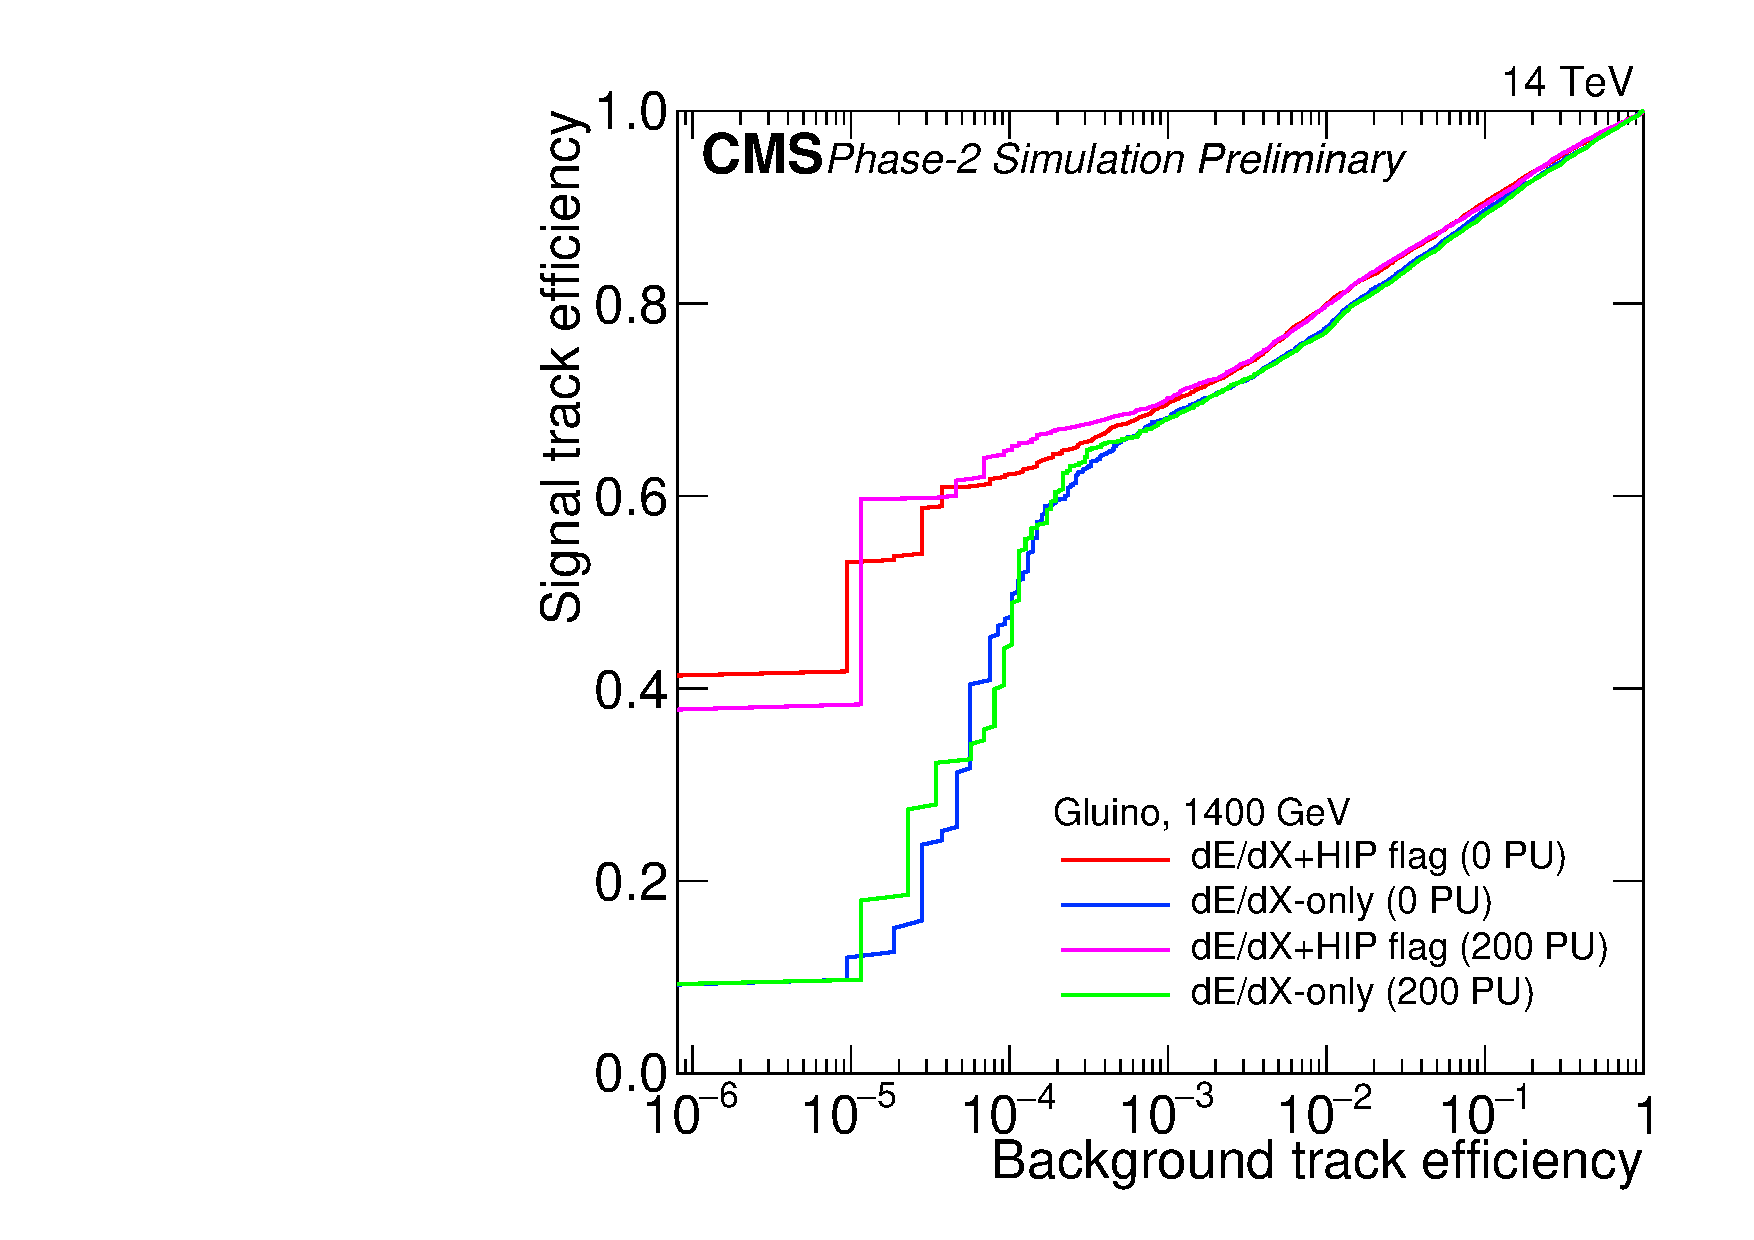
\includegraphics[width=0.47\textwidth]{figures/HSCP/TDR-17-001_fig6_27_a_HSCP_Comparison_ROC_Gluino_M1400_NoPU_Super_v2.pdf}
  \caption{ Left: distribution of the $dE/dx$ discriminator versus track momentum (p) for tracks with high momentum ($p_T > 55$~GeV) in background events (red) and for candidate signal particles. Pair produced $\tilde{\tau}_S$ with a mass of 871 GeV (blue), and a gluino with a mass of 1400 GeV (green), are shown. 
Right: The performance of the $dE/dx$ discriminator for selecting gluinos in events with 0 PU and 200 PU. The signal versus background efficiency performance curves for a discriminator making use of both the pixel information and the Outer Tracker HIP flag (red and magenta) demonstrate a better performance compared to a discriminator trained to exploit only the $dE/dx$ information from the pixel modules (blue and green), for a background rejection of $10^{-6}$. 
 }
  \label{fig:cmsupgrade_hscp}
\end{center}
\end{figure}

\paragraph{HSCP trigger with muon upgrade}

The upgrade of the RPC system will allow the trigger and identification of slowly moving particles by measuring their time of flight to each RPC station with a resolution of $\mathcal{O}(1)$~ns. The speed of muon-like particles and the time (bunch crossing) of their origin will be computed with a fast algorithm to be implemented in the Level 1 trigger at HL-LHC. 

The RPC detectors are synchronized to register muons moving at the speed of light with a local time equal to zero with respect to the collision event that produced the trigger. Slow-moving particles, as HSCPs, will arrive with a delay depending on their speed as shown in Fig~\ref{fig:hscp_time}. This time delay measured by each RPC layer crossed by the HSCP is exploited in order to trigger on and reconstruct such particles. 

\begin{figure}[h!tbp]
\begin{center}
  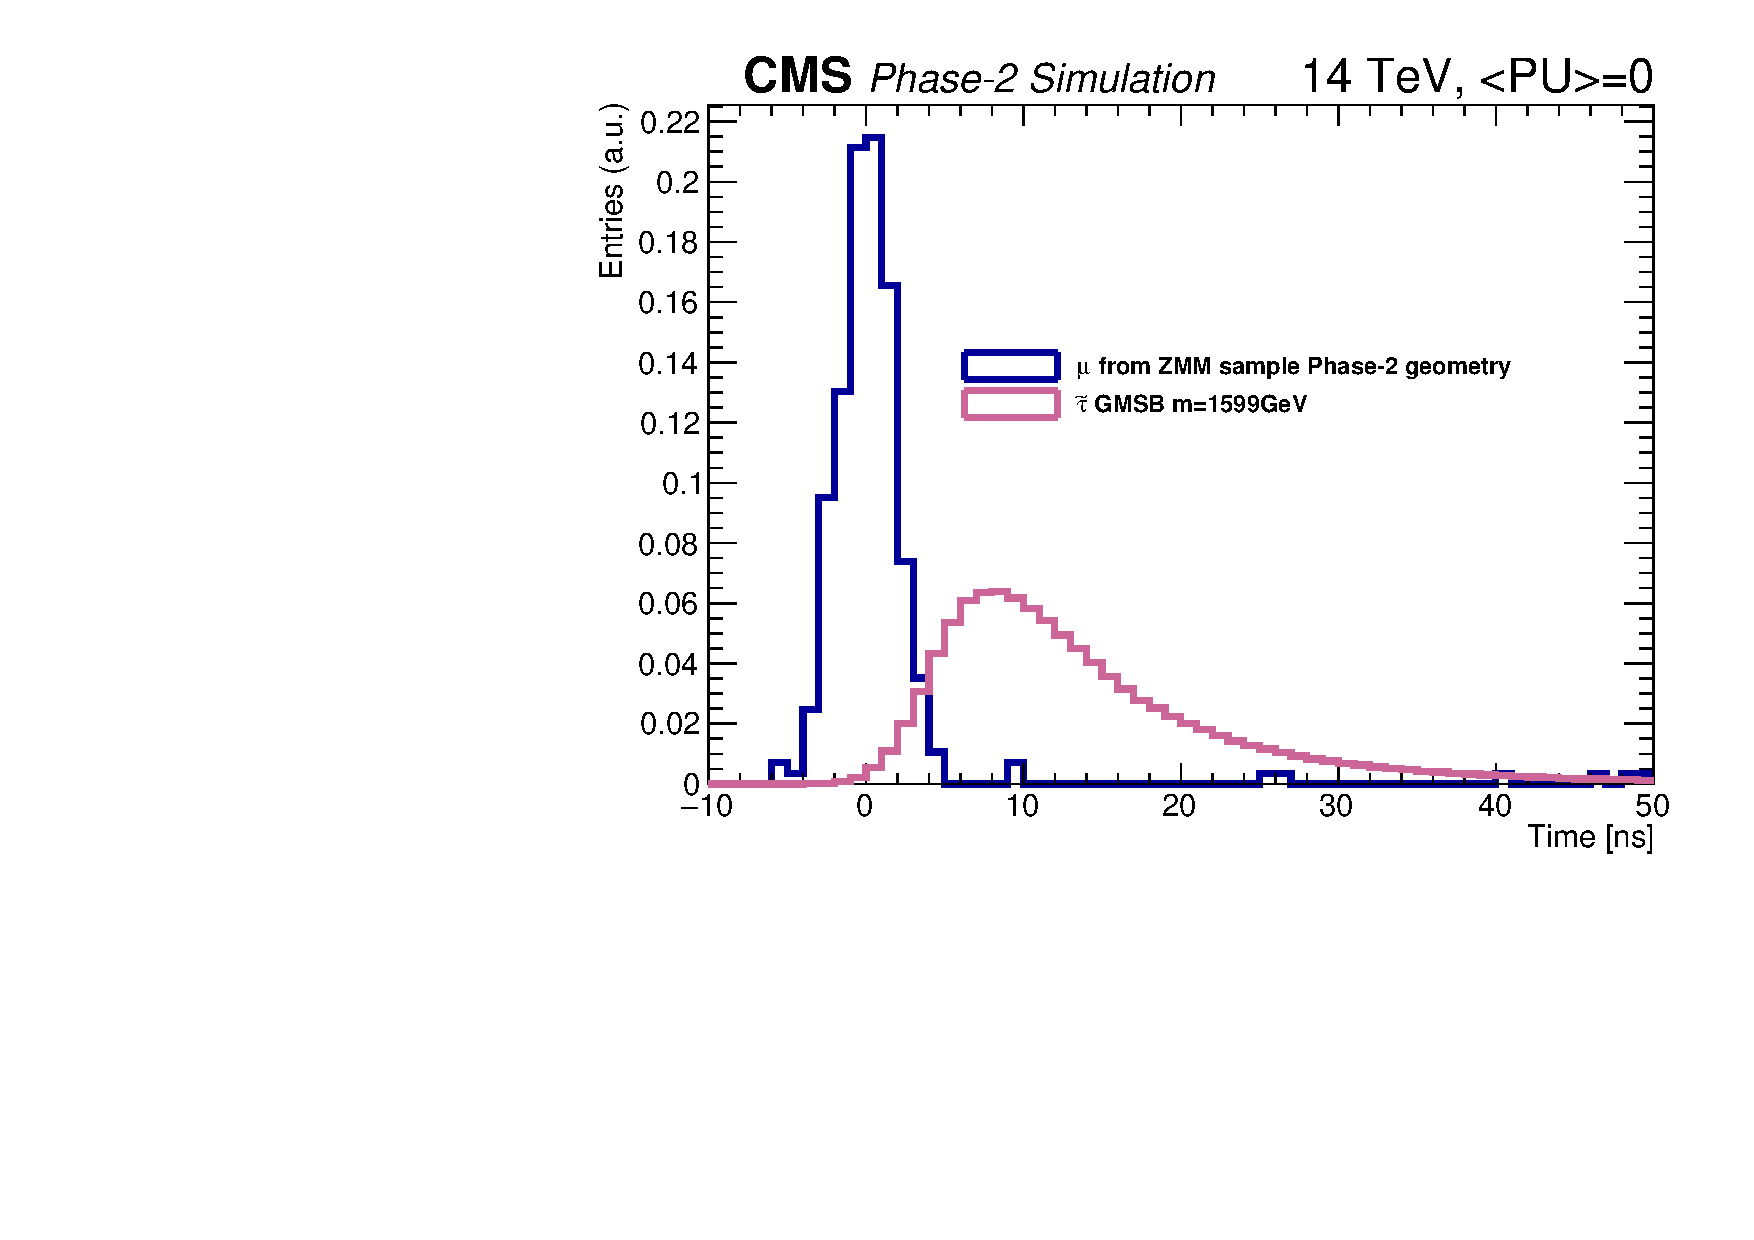
\includegraphics[width=0.7\textwidth]{figures/HSCP/time.pdf}
  \caption{RPC hit time measurement distribution for muons from $Z \to \mu\mu$ events and 
  for semi-stable $\tilde \tau$'s with m$\approx$1600\,GeV, produced in $pp \to \tilde \tau \tilde \tau$ processes. }
  \label{fig:hscp_time}
\end{center}
\end{figure}

The principles of the proposed HSCP trigger algorithm are illustrated in Fig~\ref{fig:HSCP_diagram}. In this figure, the vertical axis is the time of signals in RPC chambers, as synchronized so that muons moving nearly at the speed of light from a particular collision are measured at the time of the collision. The horizontal axis is the distance from the collision point to the position of the RPC at which the time is measured. The diagram shows three successive bunch crossings, two of which contain muons represented at horizontal lines. The diagram also shows the RPC time measurements from two HSCPs having slopes different from zero due to their traveling significantly slower than the speed of light. 
The time delay $\Delta t$ is related to the speed $v$ of an HSCP via the following equation:

\begin{equation}
\label{eq:HSCP_delay}
\Delta t = d\left(\frac{1}{v}-\frac{1}{c}\right),
\end{equation}

\noindent Here $d$ is the distance between the IP and the point where an HSCP crosses an RPC. 
For RE4/1 chambers and $\beta = v/c = 0.2$, the delay time is $>6$ BXs $= 150 \, \mathrm{ns}$.

\begin{figure}[h!tbp]
  \centering
  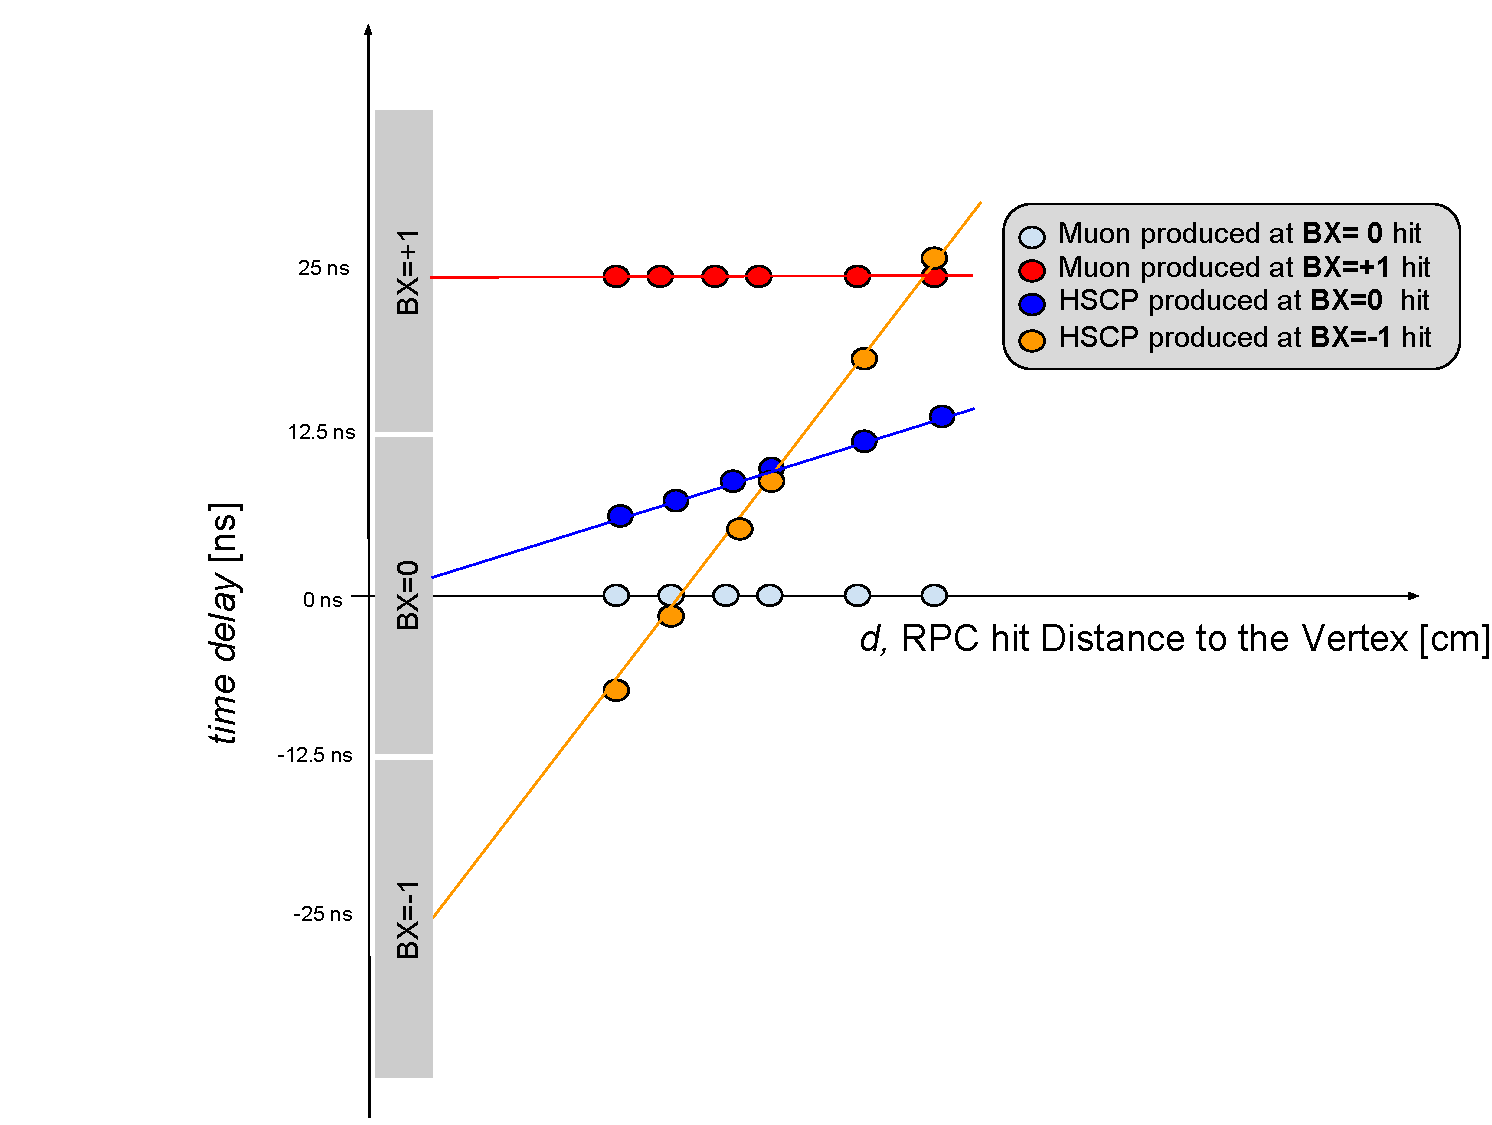
\includegraphics[width=0.6\textwidth]{figures/HSCP/diagram.pdf}
  \caption{
Diagram showing times measured at different RPC stations for particles originating at different BXs with different velocities. The $x$-axis represents the distances from IP to RPC detectors, while $y$-axis corresponds to time.
Clock at all RPC stations is tuned so that particles moving with the speed of light are registered with the exact same ``local'' times. Hence, relativistic particles are represented by horizontal lines on this diagram. 
  }
  \label{fig:HSCP_diagram}
\end{figure}


A penetrating charge particle leaves a trail of hits in RPC chambers along its trajectory.
The time of flight can be computed in each RPC station with respect to a number of BX hypotheses.
Should there be a common velocity solution, derived from Eq.~(\ref{eq:HSCP_delay}), 
with $\beta < 0.6$, a trigger is formed.
For $\beta >0.6$, the delays are small and can be handled by the Phase-1 trigger.  
The performance of this algorithm has been studied in CMS full simulation. All the detector effects 
(electronics jitter, signal time propagation along strips) are taken into account. 
A particle speed measurement resolution is shown in Fig.~\ref{fig:HCP_Trigger} (right) for the case of 25~ns
signal sampling time (Phase-1) and 1.56~ns sampling time provided with the upgraded RPC Link Board System.

\begin{figure}[h!tbp]
\begin{center}
  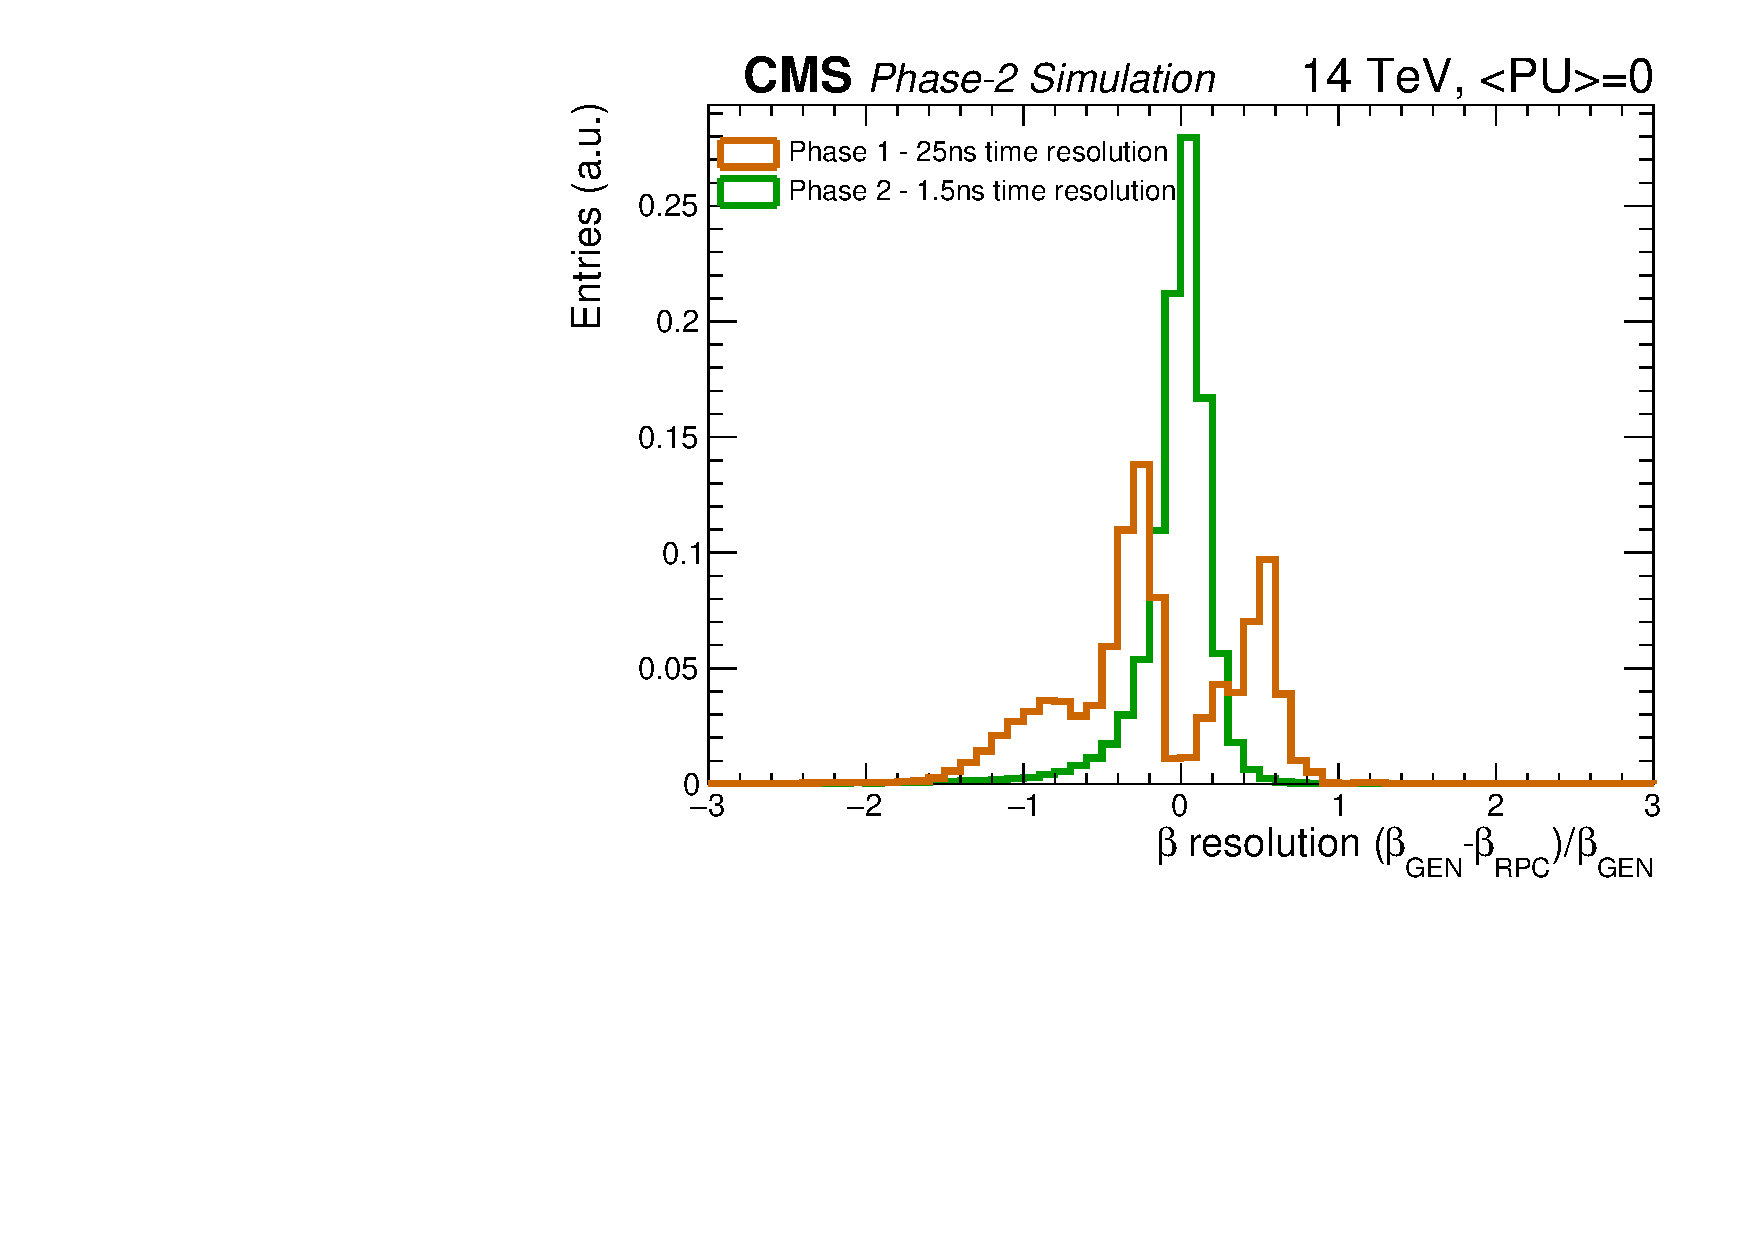
\includegraphics[width=0.47\textwidth]{figures/HSCP/beta_GenRes_2.pdf} \hfill
  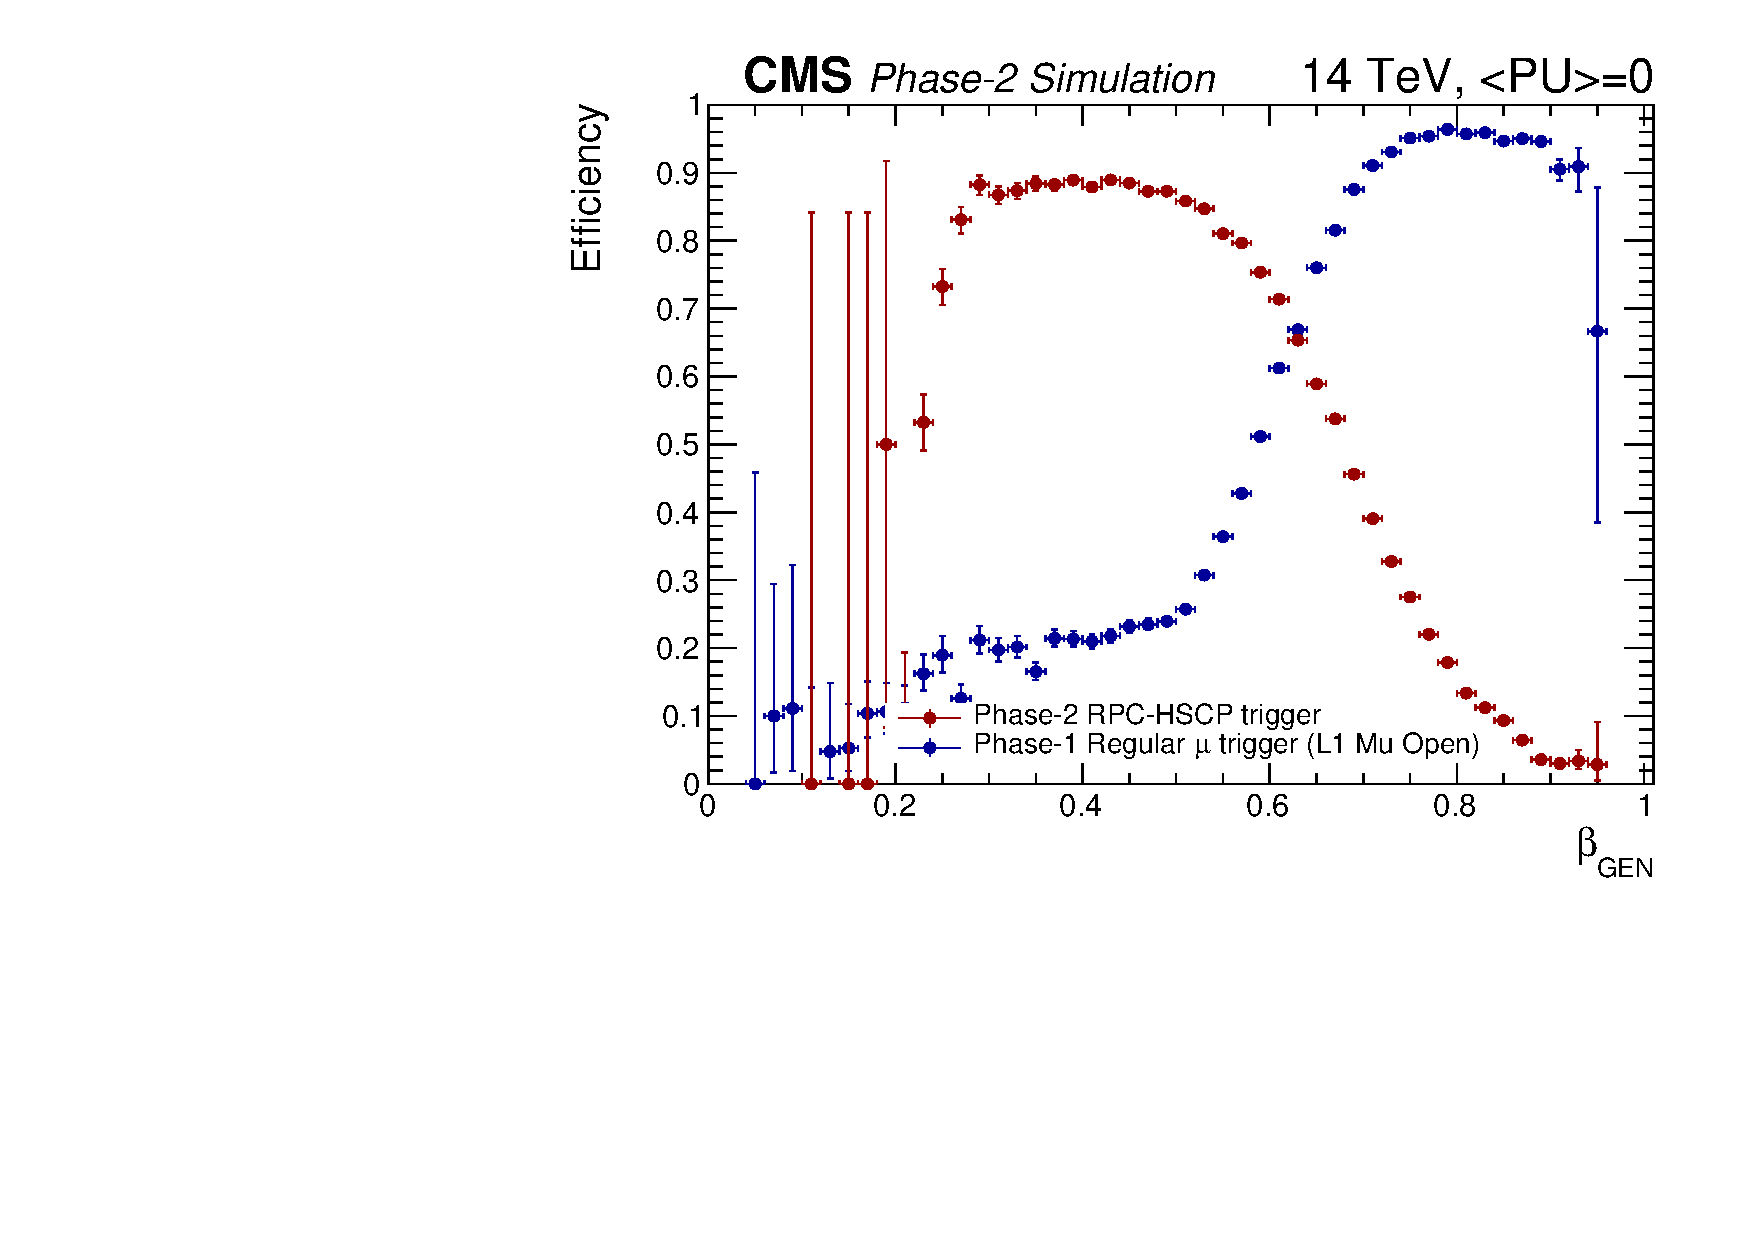
\includegraphics[width=0.47\textwidth]{figures/HSCP/trigEff-Mu-HSCPTriggers.pdf}
  \caption{
(Left) Resolution of a particle speed measurement at L1 trigger level with Phase-1 and upgraded RPC Link Board System. 
(Right) The efficiency as a function of $\beta$ of the standard L1 muon trigger without any $p_T$ threshold, 
  and the RPC-HSCP Phase-2 trigger with $1.56$~ns sampling time.
}
  \label{fig:HCP_Trigger}
\end{center}
\end{figure}

The efficiency of the RPC-HSCP algorithm as a function of $\beta$ is studied and compared with the
standard L1 muon trigger. The results are shown in Fig.~\ref{fig:HCP_Trigger} (right).
The current CMS-HSCP Phase-1 trigger performs well down to $\beta \approx 0.75$. 
The upgraded RPC Link Board System will allow us to trigger, at the
correct BX, HSCPs with velocities as low as $\beta \sim 0.25$.


Possible improvements for this trigger proposal in the $\beta$ measurement could be achieved by matching the Tracker Track trigger to the HSCP muon trigger. The uncertainty coming from the propagation time along RPC strips can be reduced if the hit position is known along the local $y$ coordinate, or the global $\eta$. This correction is not needed for the iRPCs thanks to the two-end strip readout for these new detectors.

\subsubsection{Displaced Muons} 

Many BSM theories predict particle decays with displaced muon or muon pairs in its final state, such as dark SUSY and GMSB with smuons. 
These displaced muons usually have higher $p_T$ and have been the focus of existing LLP searches. 
Their prospects at HL-LHC are discussed here. 
For models such as inelastic dark matter or dark showers that predict soft displaced muons in their final states, the reconstruction is more challenging and is discussed in Section~\ref{sec:upgradeideas}.

\paragraph{Trigger and reconstruction}

Tracks from displaced muons have different properties depending on how much the muons are boosted. 
In case of a sufficiently boosted muon, the corresponding track is roughly pointing back to the primary interaction leading to a transverse impact parameter which is small(er) but the decay may still occur at the outer edge of the tracker or even well outside the tracker volume.
If the muon is not highly boosted, the corresponding track is not pointing back to the primary interaction vertex and we might even get a large impact parameter for a decay not far away from the primary interaction.
For long-lived particles of a few hundred GeV mass, impact parameter ($|d_0|$) can
reach up to approximately one meter (or longer) for sufficiently large
lifetimes as shown in Fig.~\ref{fig:perfDisplaced} (left).

Standard triggers and reconstruction algorithms that use the position of the primary vertex will not be very efficient in reconstructing tracks with large impact parameters.
Consequently, to trigger on and reconstruct muons produced far away from the interaction vertex is challenging and requires dedicated trigger paths and reconstruction algorithms. 
As discussed in Section~\ref{sec:upgradeobject}, Fig.~\ref{fig:cmsL1mu} shows exemplarily the reconstruction capabilities of displaced muons on trigger level for the CMS detector at HL-LHC.
In the meantime, a dedicated muon reconstruction algorithm was designed for non prompt muons that leave hits only in the muon system. 
This displaced stand-alone (DSA) algorithm is seeded by groups of track segments in the muon chambers. For each seed, a muon track is reconstructed with the same Kalman-filter technique as for the standard stand-alone (SA) muon reconstruction algorithm, 
but without constraining the interaction point.
Figure~\ref{fig:perfDisplaced} (right) shows the distribution of the number of hits in the Run 2 and HL-LHC detectors for displaced muons. The impact of the new stations is clearly visible. 
The charge misidentification probability is expected to further decrease with the additional hits.

\begin{figure}[hbtp]\begin{center}
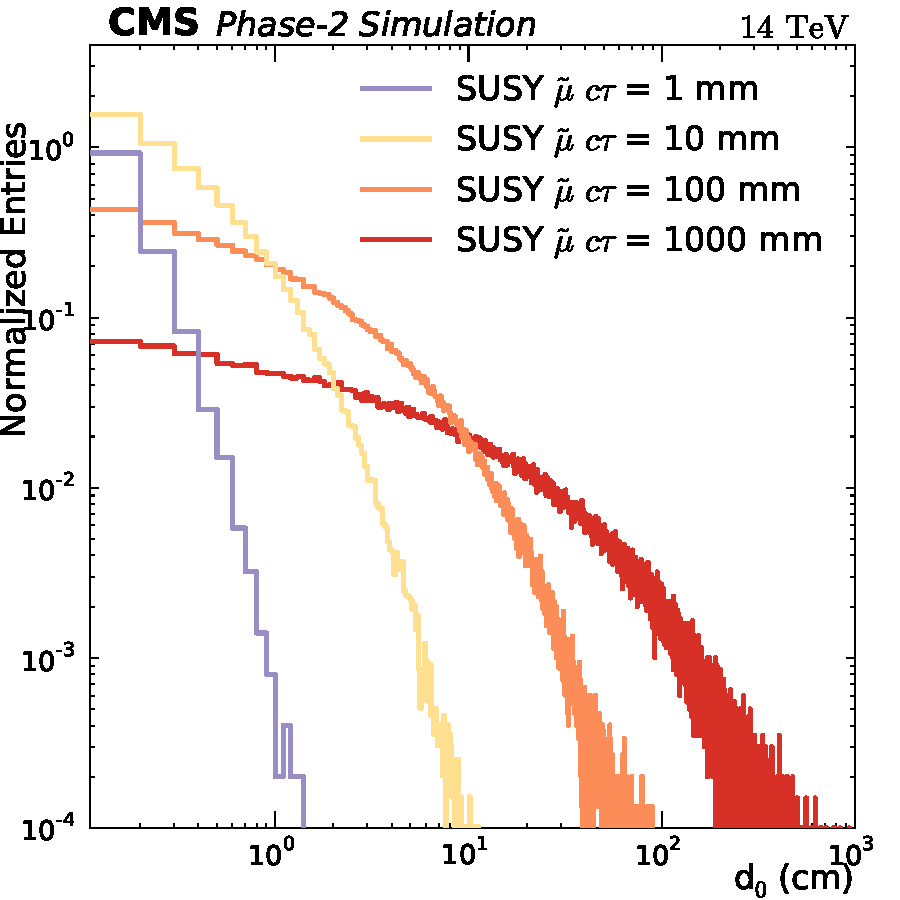
\includegraphics[width=0.47\textwidth]{figures/Stage0h1_0_d0_smuon_daughter}
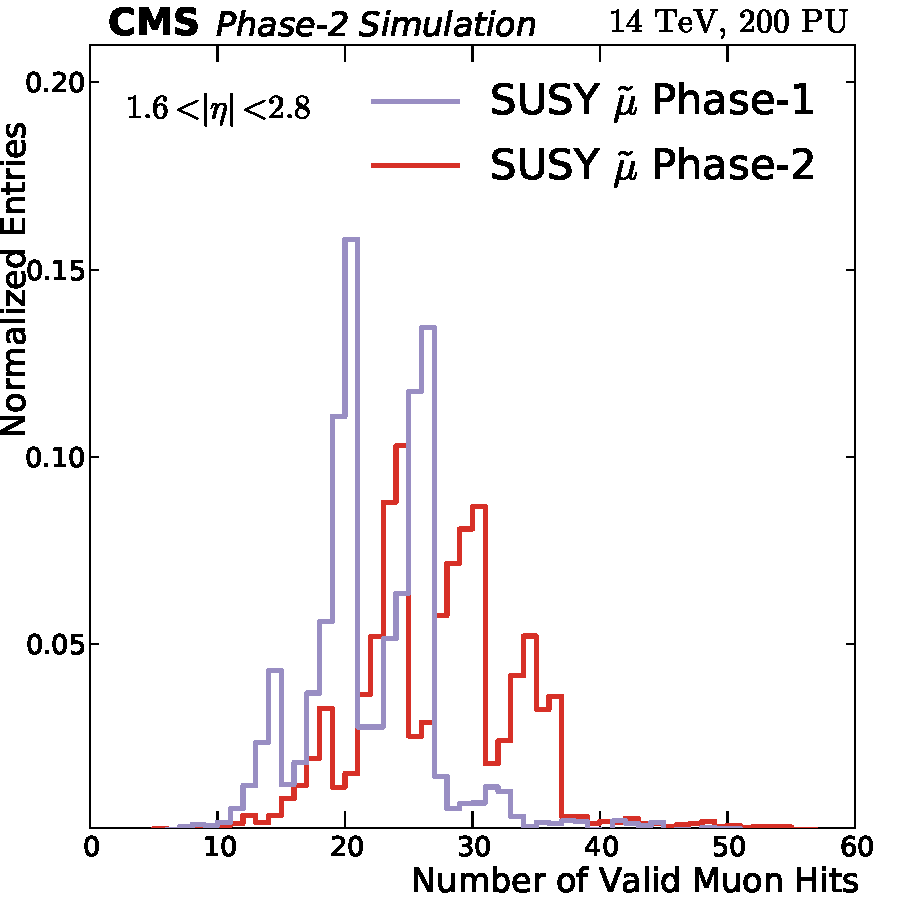
\includegraphics[width=0.47\textwidth]{figures/MuonHitsEndcap}
\caption{
Left: The transverse imparameter, $d_{0}$, for several simulated decay lengths, $c\tau$, before reconstruction.
Right: Distribution of the minimum number of valid hits in the muon system for a SUSY $\widetilde{\mu}$ (M = 500\,GeV and $\tau$ = 1000\,mm) for Run 2 (blue) and Phase-2 (red) detectors. 
}
\label{fig:perfDisplaced}
\end{center}
\end{figure}

\paragraph{Sensitivity Projection}

To study the impact on physics sensitivity, a particular gauge-mediated SUSY breaking (GMSB) model is selected where
the displaced signature consists of a dimuon final state plus gravitinos, which are escaping detection, emerging from the decay of heavy sparticles (smuons).
This signal serves as a proxy for any long-lived particle.
The final state signature is then given by two displaced oppositely charged muons 
and significant missing transverse energy which can be characterized by a very clean final-state topology.
Exemplarily long-loved particles with $c\tau=10, 100, 1000$~mm\,and with several mass hypotheses (0.2, 0.5, 1~TeV).

The main background for this search comes from multi-jet production (QCD), \ttbar~production, 
and Z/DY $\to\ell\ell$ events  where large impact parameters are (mis)reconstructed. 
Cosmic ray muons have been studied in Run 2 and are independent of the instantaneous luminosity.
In the barrel they are efficiently rejected by the timing of the hits in the upper leg. Cosmic ray muons do not originate at the vertex and therefore pass the upper barrel sectors in reverse 
direction from outside in. The fraction of cosmic ray muons in the endcaps is negligible. 
Given the very low cross section of this process, 
it is essential to reduce the background efficiently. The best background discriminator 
is the impact parameter significance $d_0 / \sigma (d_0) \geq 5$.
Given the signal kinematics, the muons should move in roughly opposite directions
and MET should be larger than $50$~GeV. 
After this selection the signal efficiency is about 4--5\% for $c\tau$~ = $1000$~mm, 
nearly independent of the smuon mass, 
and $10^{-5}$ -- $10^{-4}$ for QCD, \ttbar, and DY backgrounds.

Figure~\ref{fig:displResults} shows expected exclusion limits for the GMSB model with the smuon being a (co-)NLSP for the predicted cross section as well as for a factor 100 larger cross section. The exclusion limits are shown as functions of smuon mass in  Fig.~\ref{fig:displResults} (left) and decay length in Fig.~\ref{fig:displResults} (right).

\begin{figure}[hbtp]\begin{center}
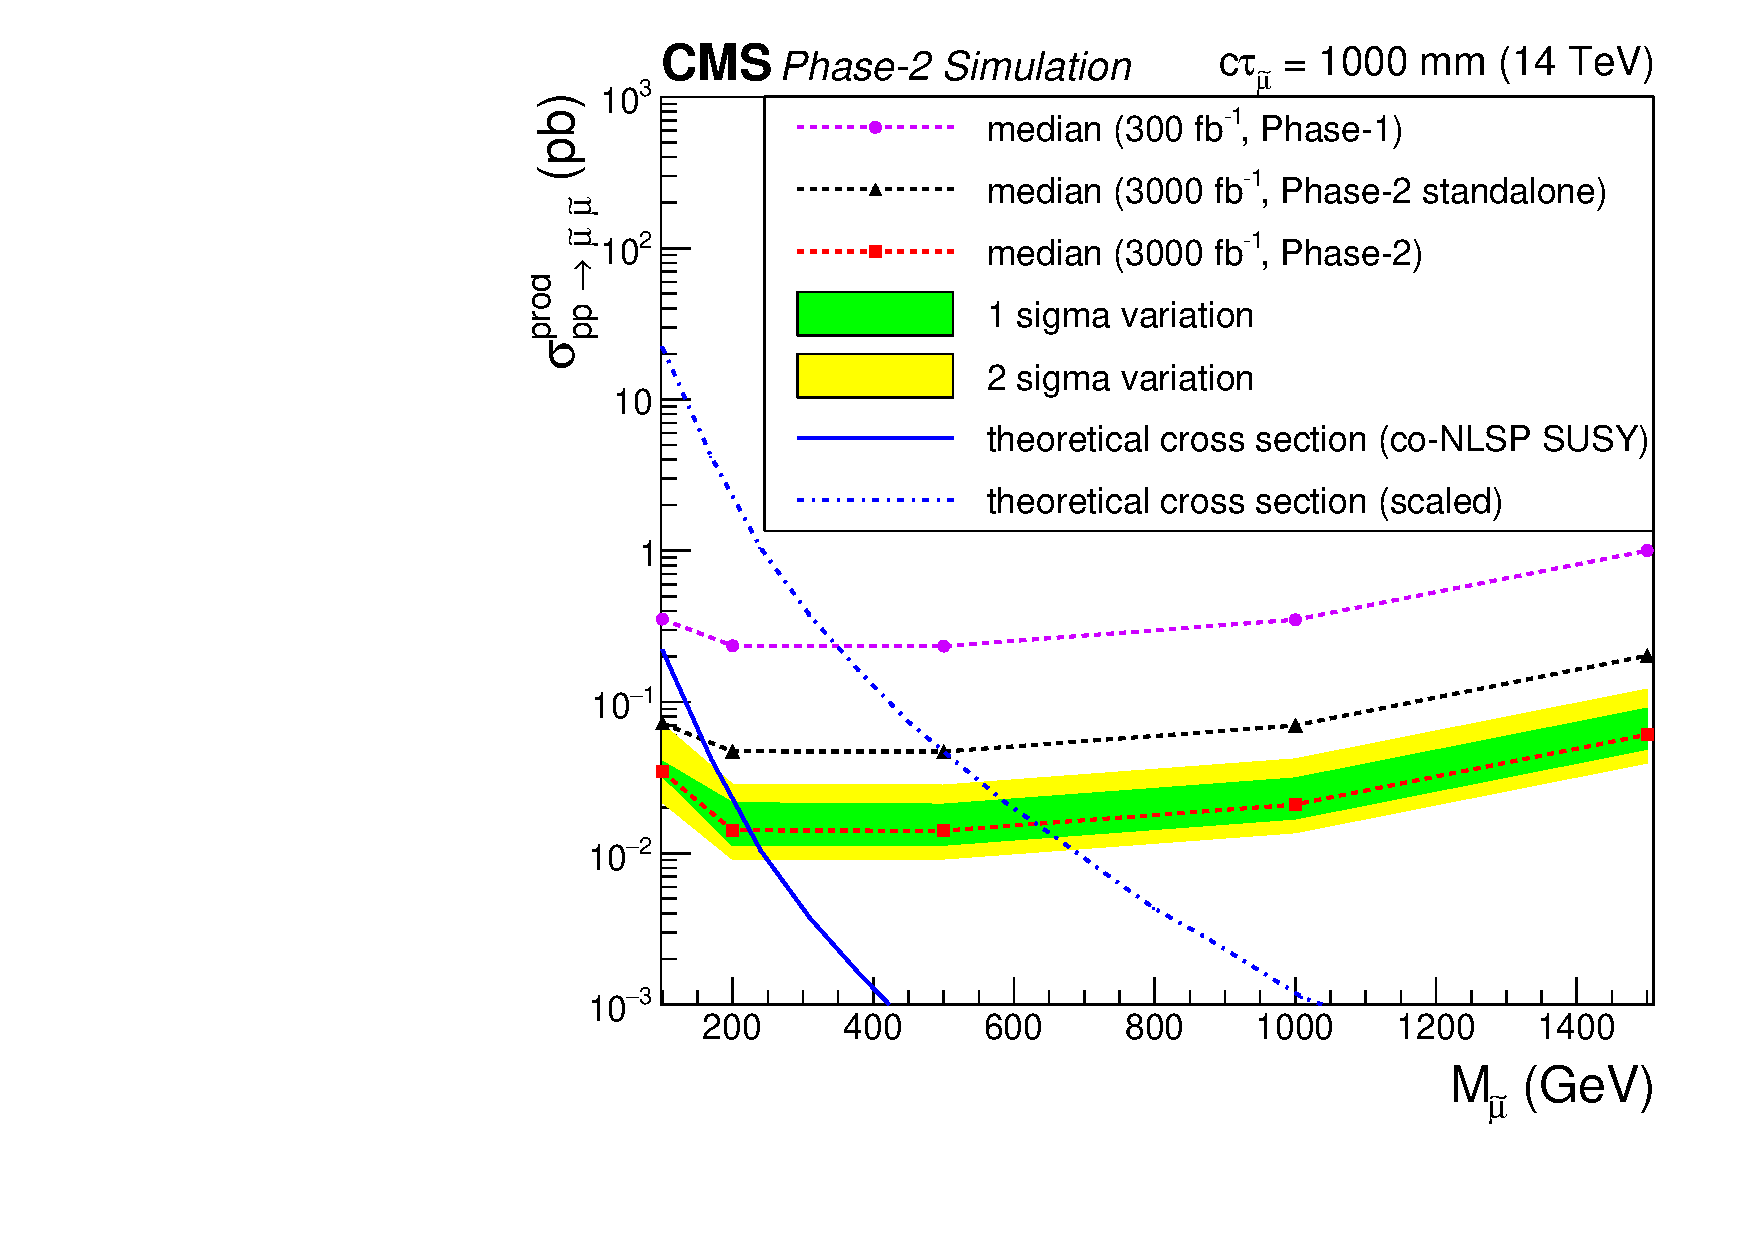
\includegraphics[width=0.49\textwidth]{figures/LimitComparison_withStandAloneEff.pdf}
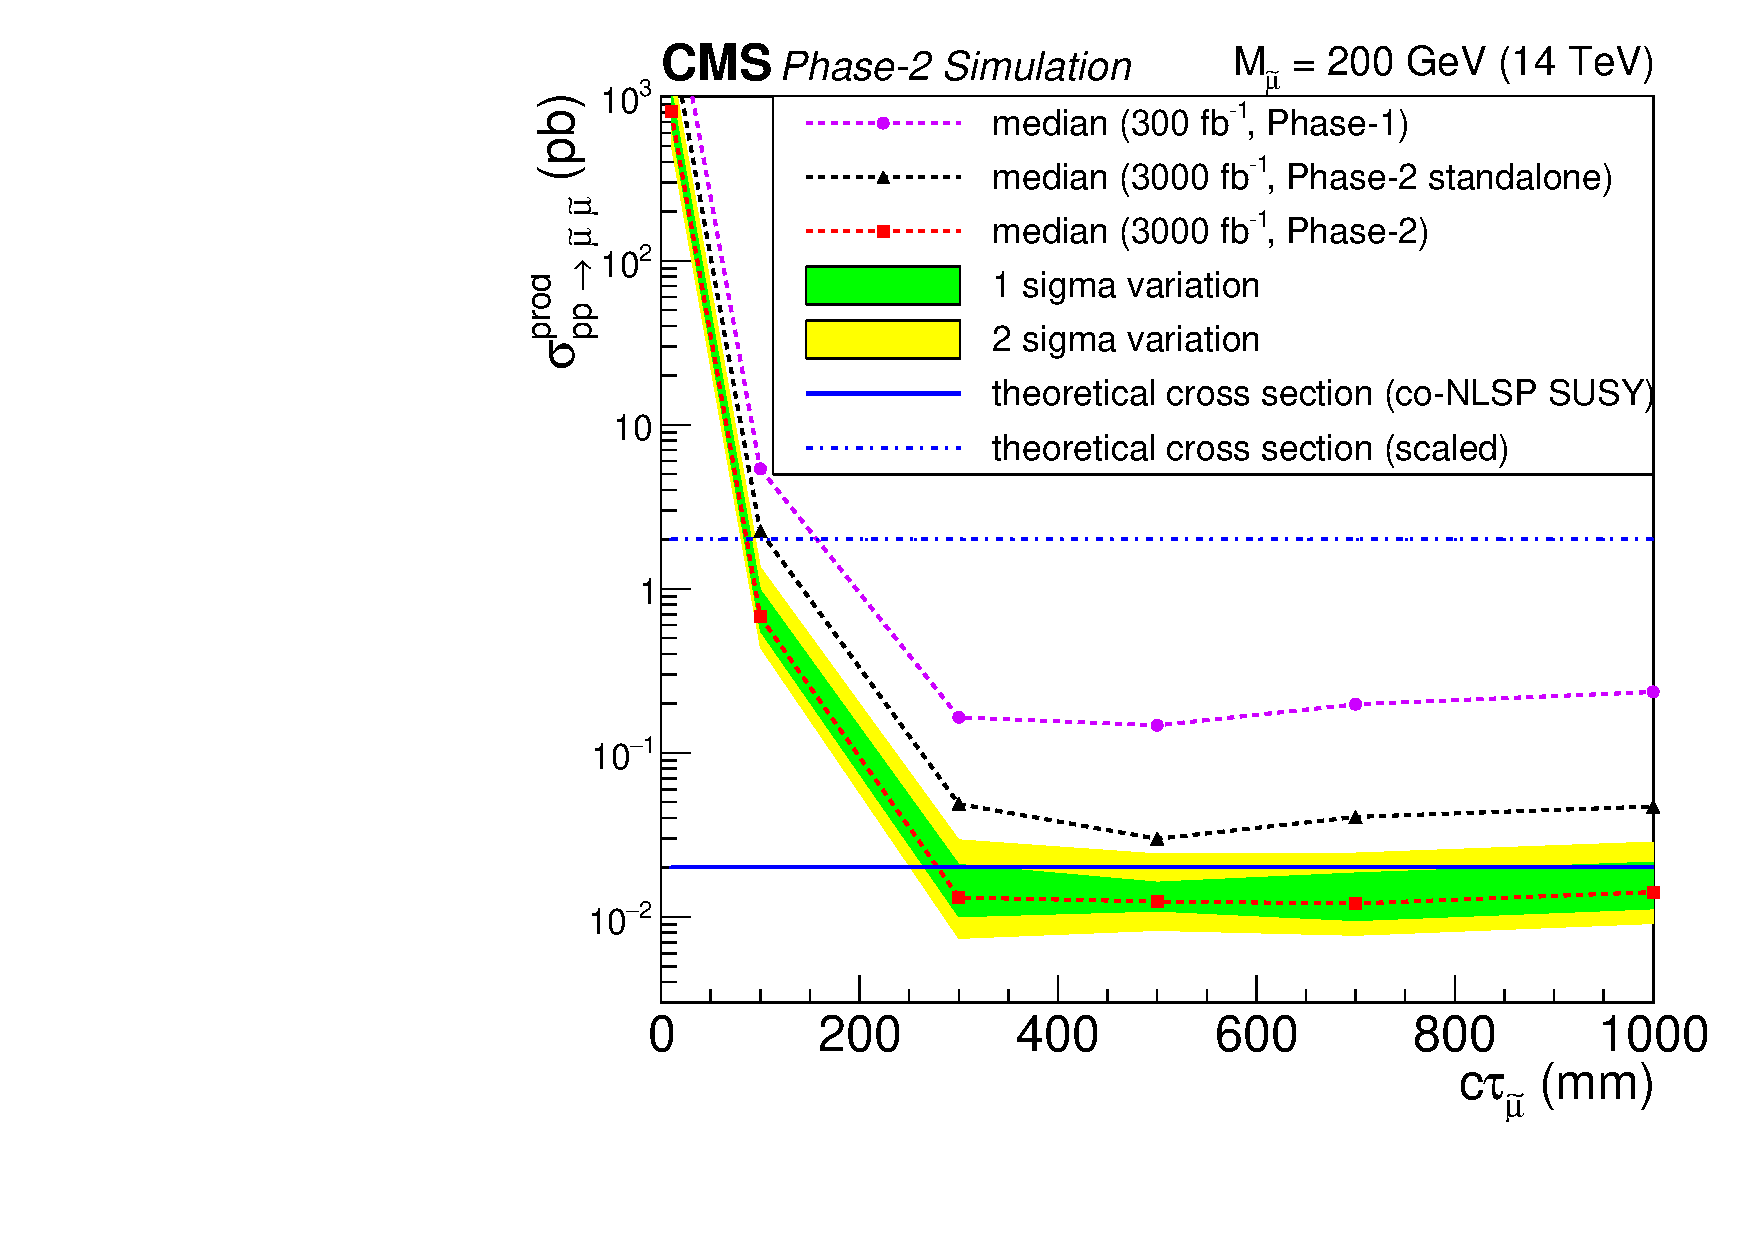
\includegraphics[width=0.49\textwidth]{figures/LimitComparison_asfuncofCtau.pdf}
\caption{The 95\% CL upper limits on  $q \bar q \to \widetilde{\mu} \widetilde{\mu}$ 
for various mass hypotheses and c$\tau$ = 1\,m (left) and as a function of the decay length for M = 200\,GeV\,(right).
In both panels, the theoretical cross section for the specific model is represented by the blue solid line.
For different SUSY breaking scales, tan $\beta$ or otherwise modified parameters, the cross sections may be  100 times larger, reflected by the blue dash-dotted line.
Green (yellow) shaded bands show the one (two) sigma range of variation of the expected 95\% CL limits. Phase-2 results with an average 200 pileup events and an integrated luminosity of 3000\fbinv are compared to results obtained with 300\fbinv. The black line shows the sensitivity without the DSA algorithm, which reduces the reconstruction efficiency by a factor three.
%%% Drop discovery significance?
%c) Discovery sensitivity for various mass hypotheses. WORKING ON IT.
 }
\label{fig:displResults}
\end{center}
\end{figure}

The sensitivity depends on $c\tau$ because shorter decay lengths shift the signal closer to background. Figure~\ref{fig:perfDisplaced} (right) shows the resulting physics sensitivities in terms of production cross section for HL-LHC, normalized to 3000\fbinv, for the dedicated reconstruction of displaced muons and for the standard reconstruction. Also shown is the expected sensitivity at the end of Phase-1.
Systematic uncertainties for the Phase-1 scenario are taken from current Run 2 analyses: 
for HL-LHC they are guided by the assumptions of reduced systematics from Ref.~\cite{FTR-16-005}.
Clearly, only the HL-LHC will allow this process to be studied. 
The expected
exclusion limit is around 200~GeV for $c\tau = 1000$~mm with 3000\fbinv.
This also illustrates the importance
of keeping lepton trigger thresholds at a few times 10~GeV, even in the environment of 200 pileup interactions.   

In order to evaluate the discovery sensitivity of a search for the GMSB model the same input is used as in the limit calculation, now with the assumption that one would have such a signal in the data. The discovery sensitivity is shown as a function of smuon mass in Fig.~\ref{fig:displResultsSensitiviy} (left) and decay length in Fig.~\ref{fig:displResultsSensitiviy}(right). The dependencies on those signal parameters are similar to the limit calculation. Analogous to the limit calculation, also the sensitivities are shown for the end of HL-LHC, normalized to 3000\fbinv, for the dedicated reconstruction of displaced muons and for the standard reconstruction. Also shown is the expected sensitivity at the end of Phase-1. 
One can conclude that only the HL-LHC is sensitive to the discovery of a long-lived particle such as the smuon with a mass higher than $200$~GeV. Another observation is the difference in discovery sensitivity for standard standalone reconstruction and dedicated displaced standalone reconstruction ranging from 1~$\sigma$ to 4~$\sigma$.

\begin{figure}[hbtp]\begin{center}
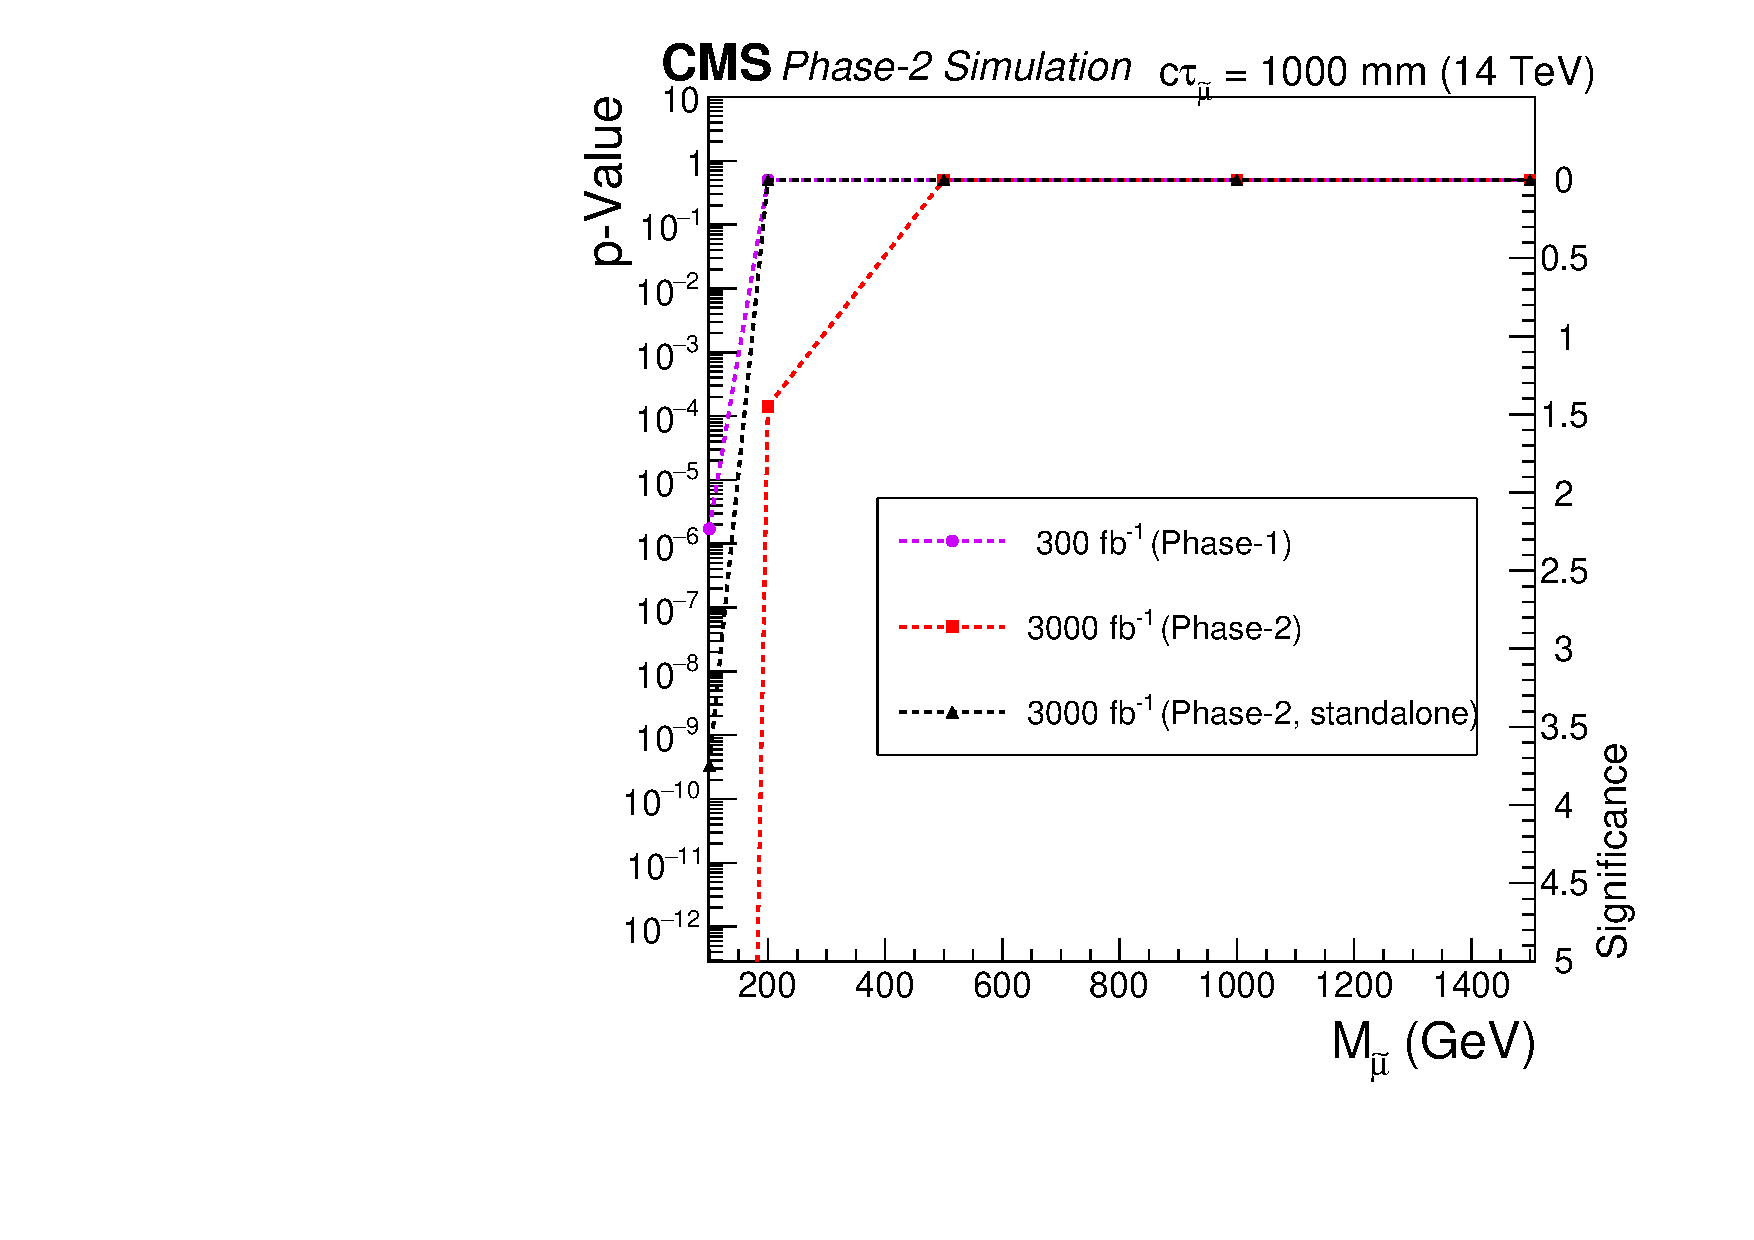
\includegraphics[width=0.49\textwidth]{figures/SignificanceComp.pdf}
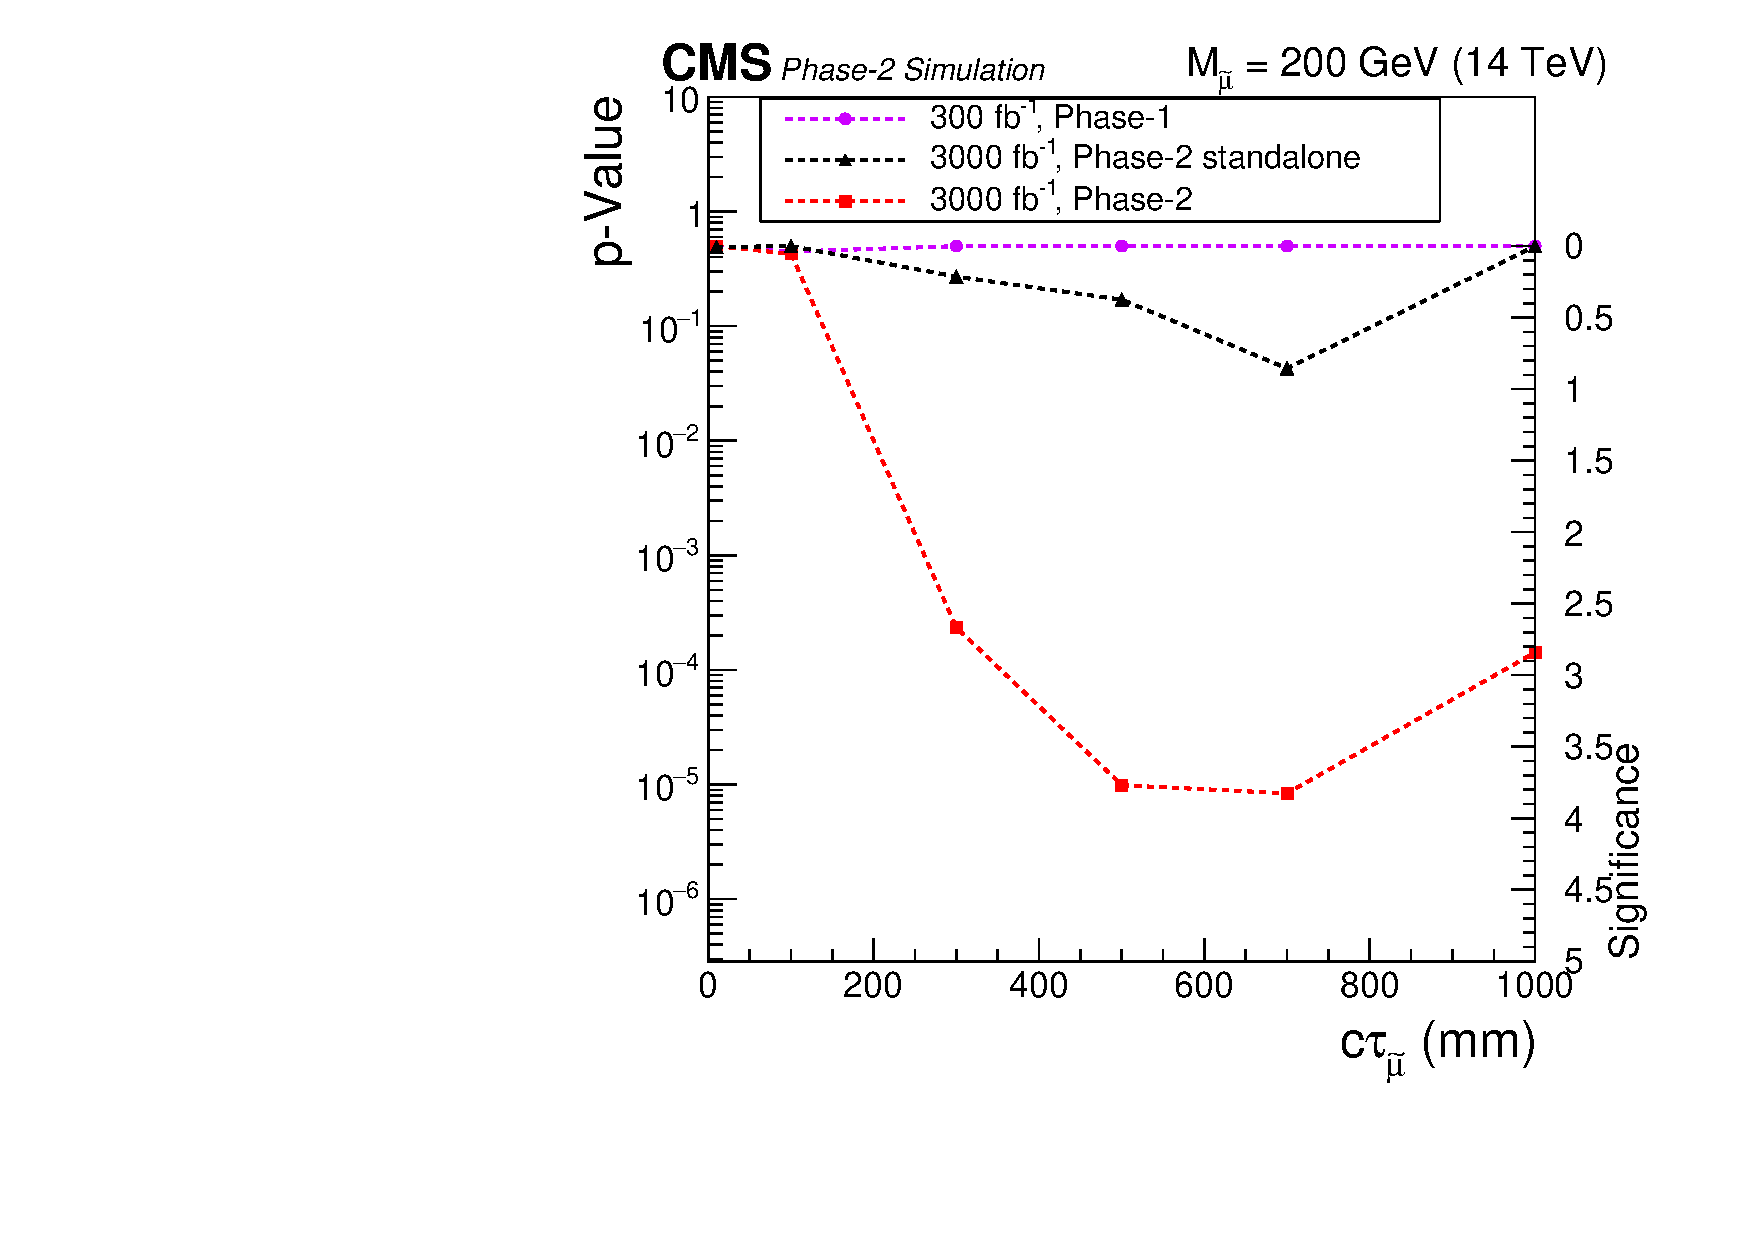
\includegraphics[width=0.49\textwidth]{figures/SignificanceComp_asfuncofCtau.pdf}
\caption{The discovery sensitivity on  $q \bar q \to \widetilde{\mu} \widetilde{\mu}$ 
for various mass hypotheses and c$\tau$ = 1\,m (left) and as a function of the decay length for M = 200\,GeV (right). Together with the discovery sensitivity the corresponding p-Value is shown. Phase-2 results with an average 200 pileup events and an integrated luminosity of 3000\fbinv are compared to results obtained with 300\fbinv. The black line shows the sensitivity without the DSA algorithm, which reduces the reconstruction efficiency by a factor three. NOT APPROVED!!!
%~ In both panels, the theoretical cross section for the specific model is represented by the blue solid line.
%~ For different SUSY breaking scales, tan $\beta$ or otherwise modified parameters, the cross sections may be  100 times larger, reflected by the blue dash-dotted line.
%~ Green (yellow) shaded bands show the one (two) sigma range of variation of the expected 95\% CL limits. Phase-2 results with an average 200 pileup events and an integrated luminosity of 3000\fbinv are compared to results obtained with 300\fbinv. The black line shows the sensitivity without the DSA algorithm, which reduces the reconstruction efficiency by a factor three.
%%% Drop discovery significance?
%c) Discovery sensitivity for various mass hypotheses. WORKING ON IT.
 }
\label{fig:displResultsSensitiviy}
\end{center}
\end{figure}


\subsubsection{Displaced Photons}

A number of new physics scenarios suggest models with displaced photons in the final state. 
At the CMS experiment, with the scintillating crystal design of the ECAL that provides excellent resolution but lacks pointing function, the photon arrival time in ECAL is the main observable used to distinguish signal from
background in displaced photon searches. 

One benchmark model for displaced photon search at collider is the GMSB model 
where the lightest neutralino ($\tilde{\chi}_0^1$) is the next-to-lightest supersymmetric particle, can be long-lived and decays to a photon and a gravitino ($\tilde{G}$), which is the LSP, as illustrated in Figure~\ref{fig:cmsupgrade_photon} (left).
For a long-lived neutralino, the photon from the $\tilde{\chi}_0^1 \to \tilde{G} + \gamma$ decay is produced at the $\tilde{\chi}_0^1$
decay vertex, at some distance from the beam line, and reaches the detector at a later time than
the prompt, relativistic particles produced at the interaction point. 
The time of arrival of the photon at the detector can be used to discriminate the signal from the background.
The aforementioned upgrade to ECAL electronics in the barrel region, and the HGCAL upgrade in the endcaps, will improve photon timing resolution at HL-LHC by an order of magnitude to as little as $\sim30$~ps for photons with $p_T$ of tens of GeV or above, hence significantly improve the experimental reach of displaced photon searches. 

Moreover, the proposed MIP Timing Detector (MTD) will be able to provide another dimension of information to reconstruct LLP decays. 
The time of flight of the photon inside the detector is the sum of the time of flight of the neutralino before its decay and the time of flight of the photon itself, until it reaches the detector.
Since the neutralino is a massive particle the latter is clearly negligible with respect to the former. 
In order to be sensitive to short neutralino lifetimes of order 1 cm, the performance of the measurement of the photon time of flight is a crucial ingredient of the analysis. 
Therefore, the excellent resolution of the MTD apparatus can be exploited to determine with high accuracy the time of flight of the neutralino, and similarly the photon, also in case of a short lifetime.

An analysis has been performed at generator level in order to evaluate the sensitivity power of a
search for displaced photons at CMS in the scenario where a 30 ps timing resolution is available from the MTD. The events were generated with Pythia8, exploring neutralino lifetimes ($c\tau$) explored in the range 0.1-300 cm. 
The values of the $\Lambda$ scale parameter were considered in the range 100-500 TeV, which is relevant for this model to be consistent with the observation of a 125 GeV Higgs boson. 
After requiring the neutralino decaying within the CMS ECAL acceptance and the photon energy being above a ``trigger-like" threshold, the generator-level photon time of flight was smeared according to the expected experimental resolutions. A cut
off at a photon time greater than 3s of the time resolution is applied and the ``signal region" is assumed to be background free. The signal efficiency of such a requirement is computed and translated, assuming the theoretical cross sections provided in Ref~\cite{ref:GMSB}, to an upper limit at 95% CL on the production cross section of the $\tilde{\chi}_0^1 \to \tilde{G} + \gamma$ process. 

Figure~\ref{fig:cmsupgrade_photon}(right) shows the analysis sensitivity in terms of the L scale (and therefore of the neutralino mass) and lifetime for three different assumptions on the timing resolution. 
The 300 ps resolution is representative of the time-of-flight resolution (TOF) for these events with current CMS detector performance]. 
The 180 ps resolution is representative of the TOF resolution of the upgraded CMS detector without the MTD, in which the TOF measurement will be dominated by the time spread of the luminous region. 
The vertex timing provided by the MTD detector will bring the TOF resolution to about 30 ps. 
As visible in the figure, a full scope upgrade of the CMS detector with photon and track timing will provide a dramatic increase in sensitivity at short lifetimes and high masses, already after the first $300 fb^{-1}$ of integrated luminosity.

\begin{figure}[hbtp]\begin{center}
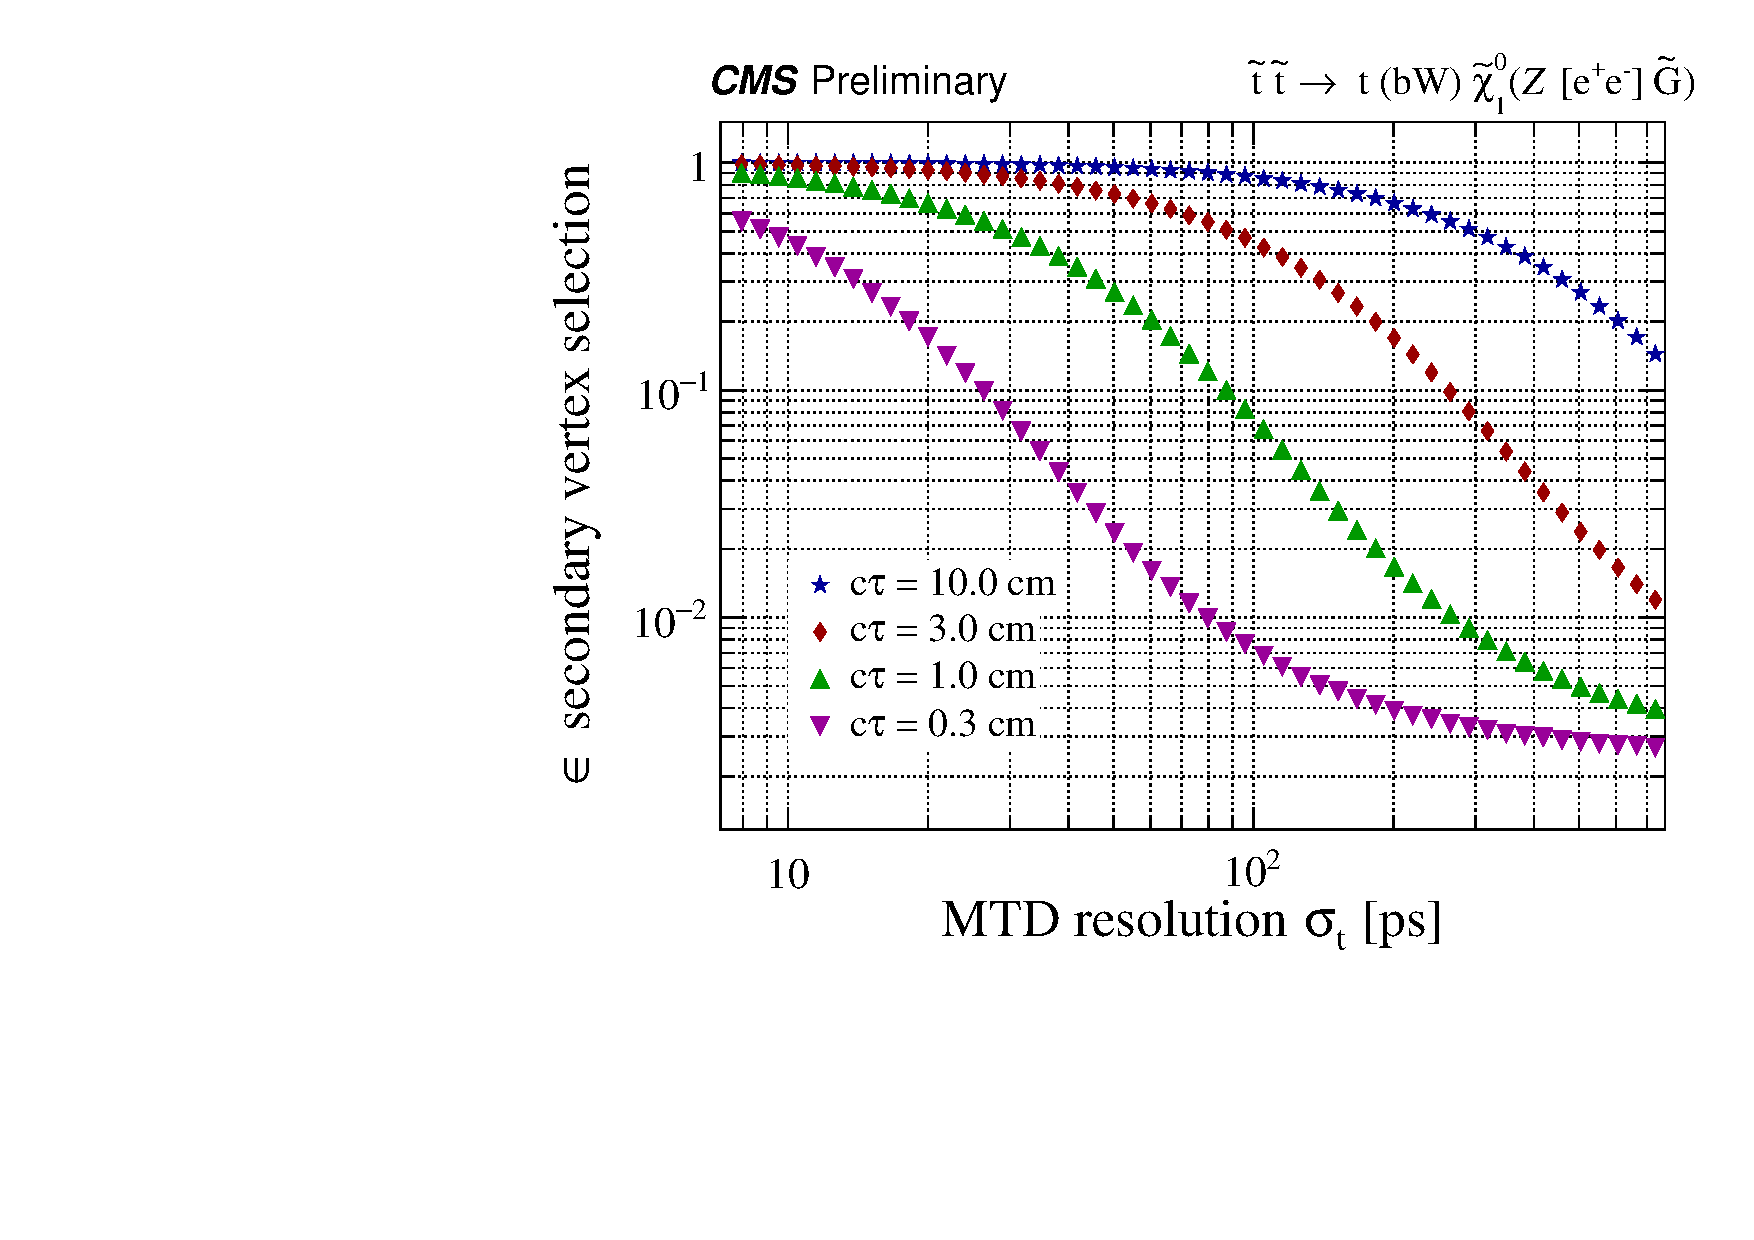
\includegraphics[width=0.47\textwidth]{figures/MTD/171025_52.pdf}
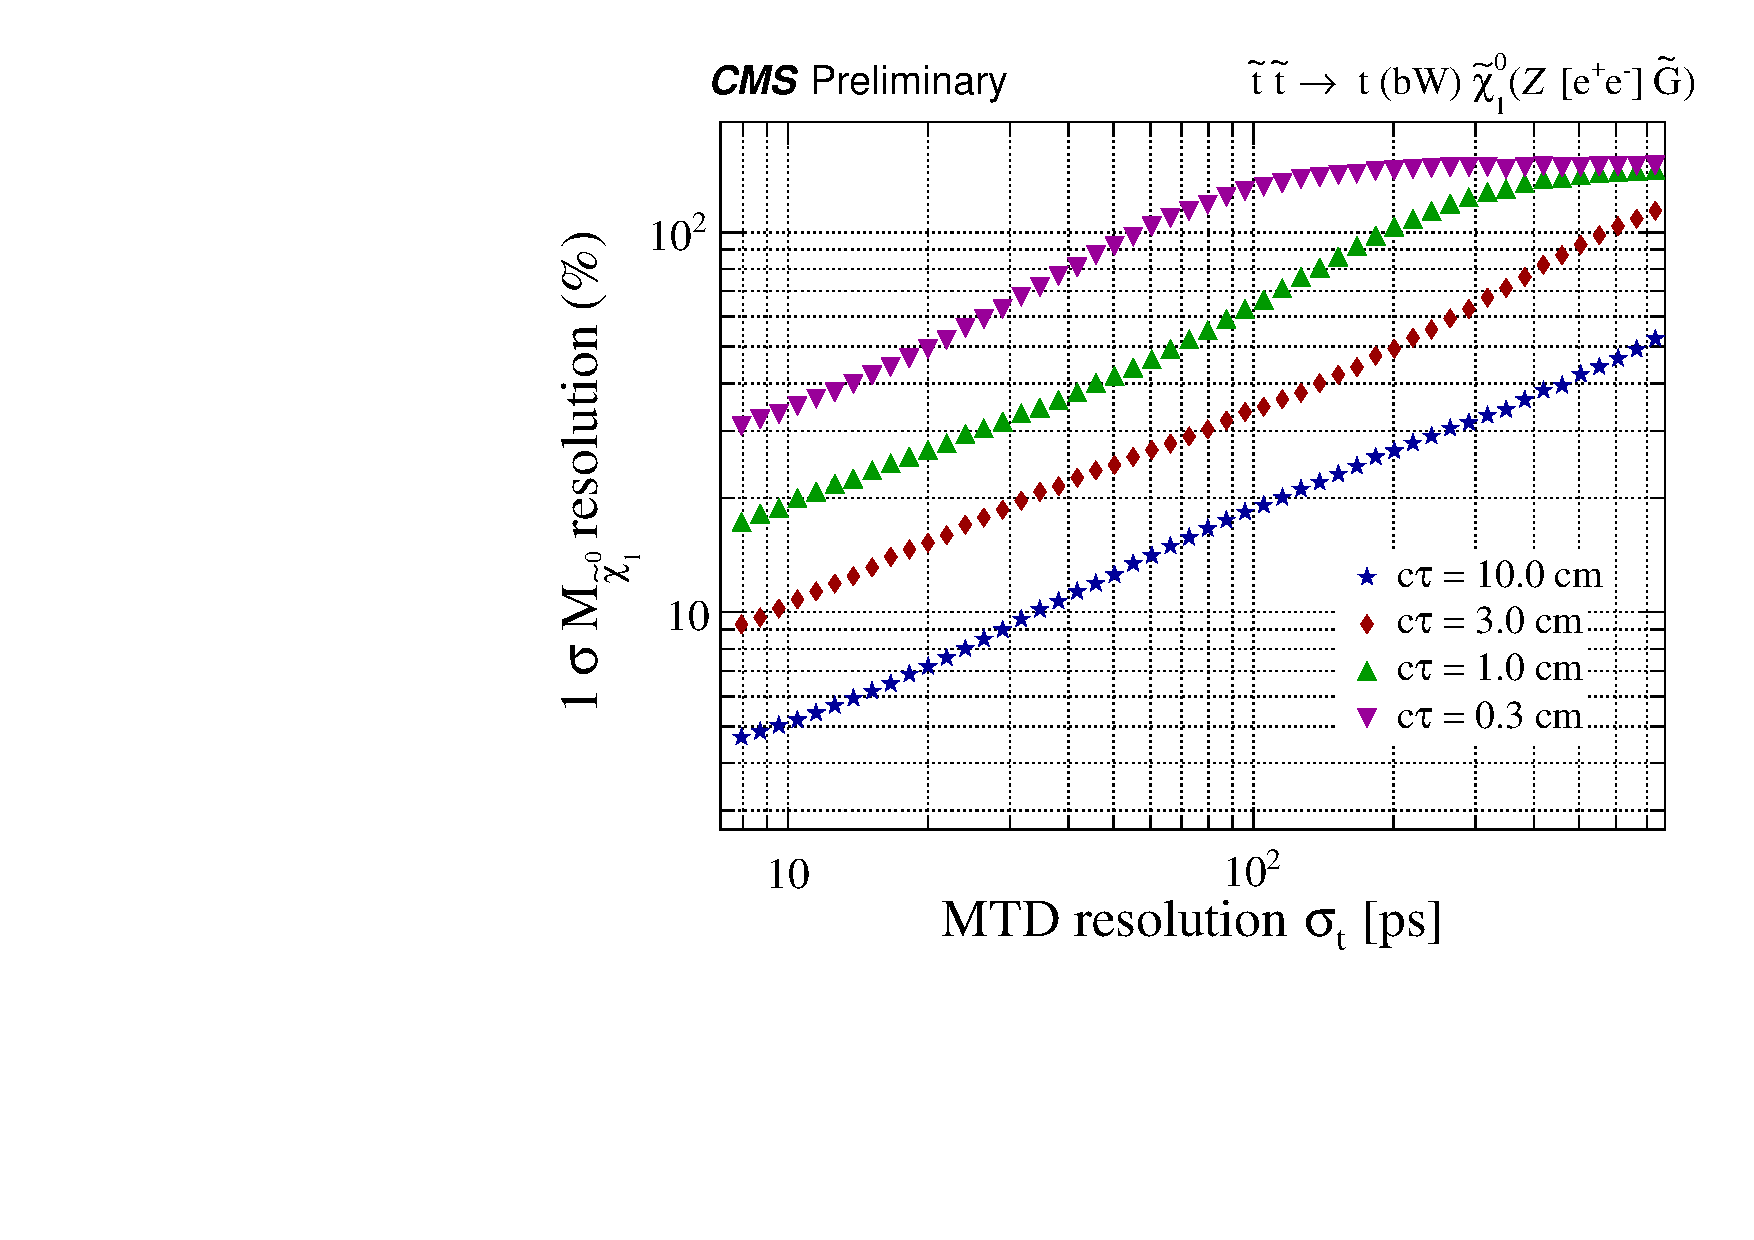
\includegraphics[width=0.47\textwidth]{figures/MTD/171025_53.pdf}
\caption{ 
Left: Diagrams for a SUSY process that results in a diphoton final state through gluino production at the LHC. 
Right: Sensitivity to GMSB $\tilde{\chi}_0^1 \to \tilde{G} + \gamma$ signals expressed in
terms of neutralino lifetimes for 300, 180 and 30 ps resolution, corresponding to the current
detector, the HL-LHC detector with photon timing without MTD and with MTD, respectively.
}
\label{fig:cmsupgrade_photon}
\end{center}
\end{figure}


\subsubsection{LLP searches with precision timing}

The MTD provides new, powerful information in searches for long-lived particles. 
A precision MIP timing detector allows one to assign timing for each reconstructed vertex and to measure the time of flight of LLPs between primary and secondary vertices. 
Using the measured displacement between primary and secondary vertices in space and time, the velocity of an LLP in
the laboratory frame, $\vec{\beta}_{LAB}^{p}$ (and $\gamma^p$), can be measured. In such scenarios, the LLP can decay to fully-visible or partially-invisible systems. 
Using the measured energy and momentum of the visible portion of the decay, one can calculate its energy in the LLP rest frame and reconstruct the mass of the LLP, assuming that the mass of the invisible system is known. 

In addition to the aforementioned GMSB displaced photon model, the benefits of precision timing with the MTD can be further demostrated in SUSY scenarios where the LLP decay produces a Z boson, which then decays to an electron-positron pair.
For example, in the GMSB scenario where the $\tilde{\chi}_0^1$ couples
to the gravitino $\tilde{G}$ via higher-dimension operators sensitive to the SUSY breaking scale, the $\tilde{\chi}_0^1$ may have a long lifetime. 
It is produced in top-squark pair production with 
$\tilde{t}\to t+\tilde{\chi}_0^1$, $\tilde{\chi}_0^1 \to Z+\tilde{G}$, $Z\to ee$.

Studies are performanced to estimate the sensitivity of the search with the MTD.
The events were generated with Pythia8. The masses of the top-squark and neutralino were set to 1000 GeV and 700 GeV, respectively. 
Generator-level quantities were smeared according to the expected experimental resolutions. 
A position resolution of 12 mm in each of the three spatial directions was assumed for the primary vertex.
 The secondary vertex position for the electron-positron pair was reconstructed assuming 30 mm track resolution in the transverse direction. 
The momentum resolution for electrons was assumed to be $2\%$. 
And finally, the time resolution of charged tracks at the displaced vertex were assumed to be 30 ps.

The mass of the LLP was reconstructed assuming that the gravitino is massless. The fraction of events with separation between primary and secondary
vertices exceeding 3s in both space and time as a function of the MTD resolution is shown in
Figure~\ref{fig:cmsupgrade_mtd} (left). The mass resolution, defined as half of the shortest mass interval that contains $68\%$ of events with 3s displacement is shown in Figure~\ref{fig:cmsupgrade_mtd}(right), 
as a function of the MTD resolution. 

\begin{figure}[hbtp]\begin{center}
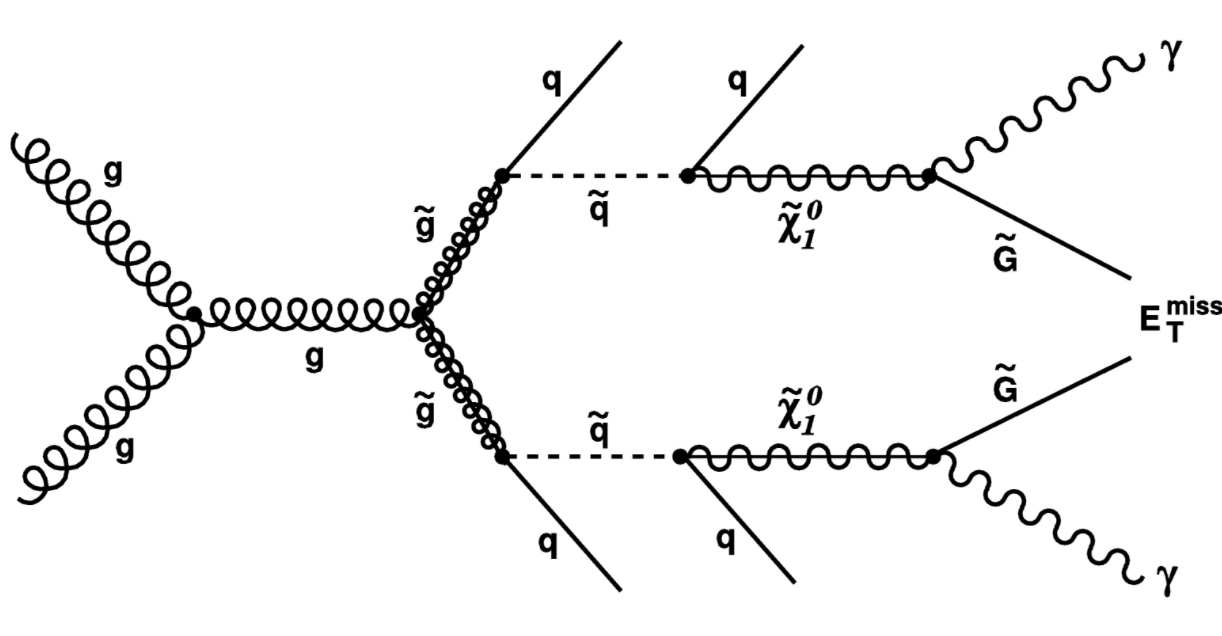
\includegraphics[width=0.47\textwidth]{figures/MTD/diagram.png}
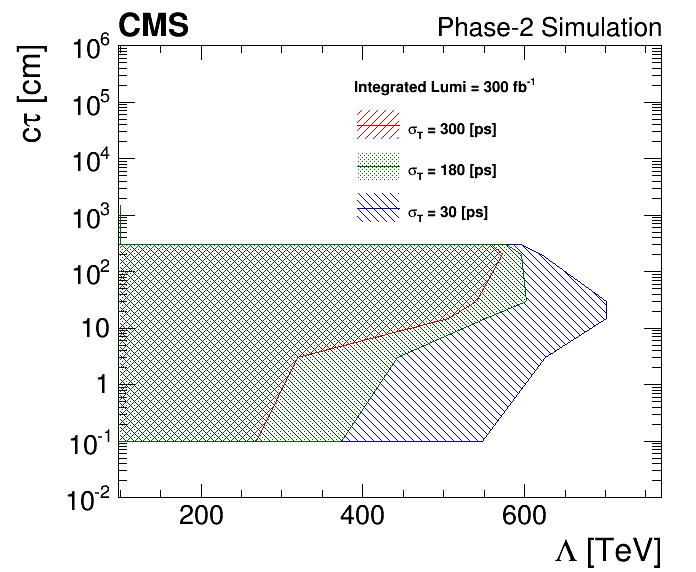
\includegraphics[width=0.47\textwidth]{figures/MTD/Limits_excl_2D_ComparingRes.png}
\caption{ 
Efficiency (left) and mass resolution (right) as a function of the timing resolution of the MTD for reconstruction of the $\tilde{\chi}_0^1$ mass in the SUSY GMSB example of $\tilde{\chi}_0^1 \to \tilde{G} e^{+} e^{-}$, with
mass of $\tilde{\chi}_0^1=700$~GeV, considering events with a separation of primary and secondary vertices by more than 3s in both space and time.
}
\label{fig:cmsupgrade_mtd}
\end{center}
\end{figure}

A similar study is done with another SUSY scenario where the two lightest neutralinos and light chargino are higgsino-like. The light charginos and neutralinos are nearly mass degenerate and
may become long-lived as a consequence of the heavy higgsinos. 
In both studies, the additional timing information from the MTD facilitates the reconstruction of the LLP mass, the resolution and efficiency of which are further improved with the excellent timing resolution of the MTD.


\subsubsection{LLP searches with track trigger}

As discussed in Section~\ref{sec:upgrademachine}, a central feature of the CMS upgrade at HL-LHC is a new silicon outer tracker which allows track reconstruction for every LHC bunch crossing (40 MHz). 
The $p_T$ selection for stubs (hit pairs in the $p_T$ modules of the outer tracker) to be read out is determined by the bandwidth from the detector 
to the back end electronics, and is fixed at about 2 GeV. 
On the other hand, the choice of track finding algorithm and hardware is still being finalized, and there could be significant benefits to extend the L1 track trigger ability to off-pointing tracks. 

To illustrate the case, a simple toy simulation (Ref.~\cite{Gershtein:2017tsv}) to study rare Higgs decays into new particles with lifetime of order of a few mm is performed. 
This study considers all-hadronic final states with low $H_T$, taking SM Higgs decays into four jets as an example.
Theoretical motivation to look for such decays is very strong, The goal is to probe very small
branching fractions; in this note we assume $Br[h\rightarrow\phi\phi\rightarrow 4q] = 10^{-5}$. 
For prompt decays, the background is overwhelming, but if the $\phi$ has $c\tau$ of a few mm, the offline analysis has very low 
backgrounds.
The problem is in getting such events on tape, in particular through L1. This toy study estimates how an off-pointing track reconstruction 
at L1 can help. To estimate the efficacy of the approach, the result projections are compared with the best alternatives in absence of off-pointing track trigger: using
associated Higgs production with a W that provides a lepton trigger or considering L1 calorimeter jets with no associated 
prompt tracks.

This study is simulated with a toy tracker, which has six perfectly cylindrical double layers \cite{geom} covering $|\eta|<2.4$. 
For each layer, the allowed offset between the two measurements
is below the one expected from 2 GeV prompt tracks. 
The sketch in Figure~\ref{fig:tracktrigger_toy} (left) shows four tracks traversing a double layer: positively and negatively charged 
prompt 2 GeV tracks, and two off-pointing tracks. Dashed track would make a L1 trigger stub, and the dotted one would not. 

Two extensions of track finder are considered. {\it Loose} tracks are only required to have a minimal number of stubs. 
{\it Tight} tracks are obtained by fitting the stubs they produced to a circle constrained to the beam line. The number of stubs on a tight track
is the number of stubs deviating from that circular fit by less then 3 strips (300 microns). Tight tracks is a generous approximation for 
an algorithm that assumes prompt production when building a track and allows for non-zero impact parameter for track fit.
For loose tracks, both track building and fitting assumes non-zero impact parameter. We only consider the transverse plane of the track finding
since that's the plane in which the displacement is measured more precisely. We assume that the hits on a track are also linked in the $rz$, but do 
not rely on it for calculation of displacement. 

The $h\rightarrow\phi\phi\rightarrow 4q$ events were generated using PYTHIA. Mass of $\phi$ is taken to be 30 GeV,
and $Br[h\rightarrow\phi\phi\rightarrow 4q]=10^{-5}$. A range of $\phi$ lifetimes is considered, from 1 mm to 5 m.
Proper decay time was randomly generated for each $\phi$ and dilated according to its speed.

Figure~\ref{fig:tracktrigger_toy} (right) shows the expected event yields for different triggers described above.
Jet reconstruction parameters were slightly varied to make sure there are no large variations in efficiency.
For track jets, one (solid lines) or two (dashed lines) tracks with five or more hits were required.
For trackless jets, one track (solid line) or two tracks with total $p_T$ below 10 GeV were allowed to to point along the jet.

While the tight tracks offer substantial increase in sensitivity compared to $Wh$, trigger based on loose tracks  
yields more then a factor of 5 more signal for $c\tau$ of a few mm. No-track jets, even with very optimistic 70 GeV threshold
only become competitive at lifetimes of 50cm or more.

\begin{figure}[hbtp]\begin{center}
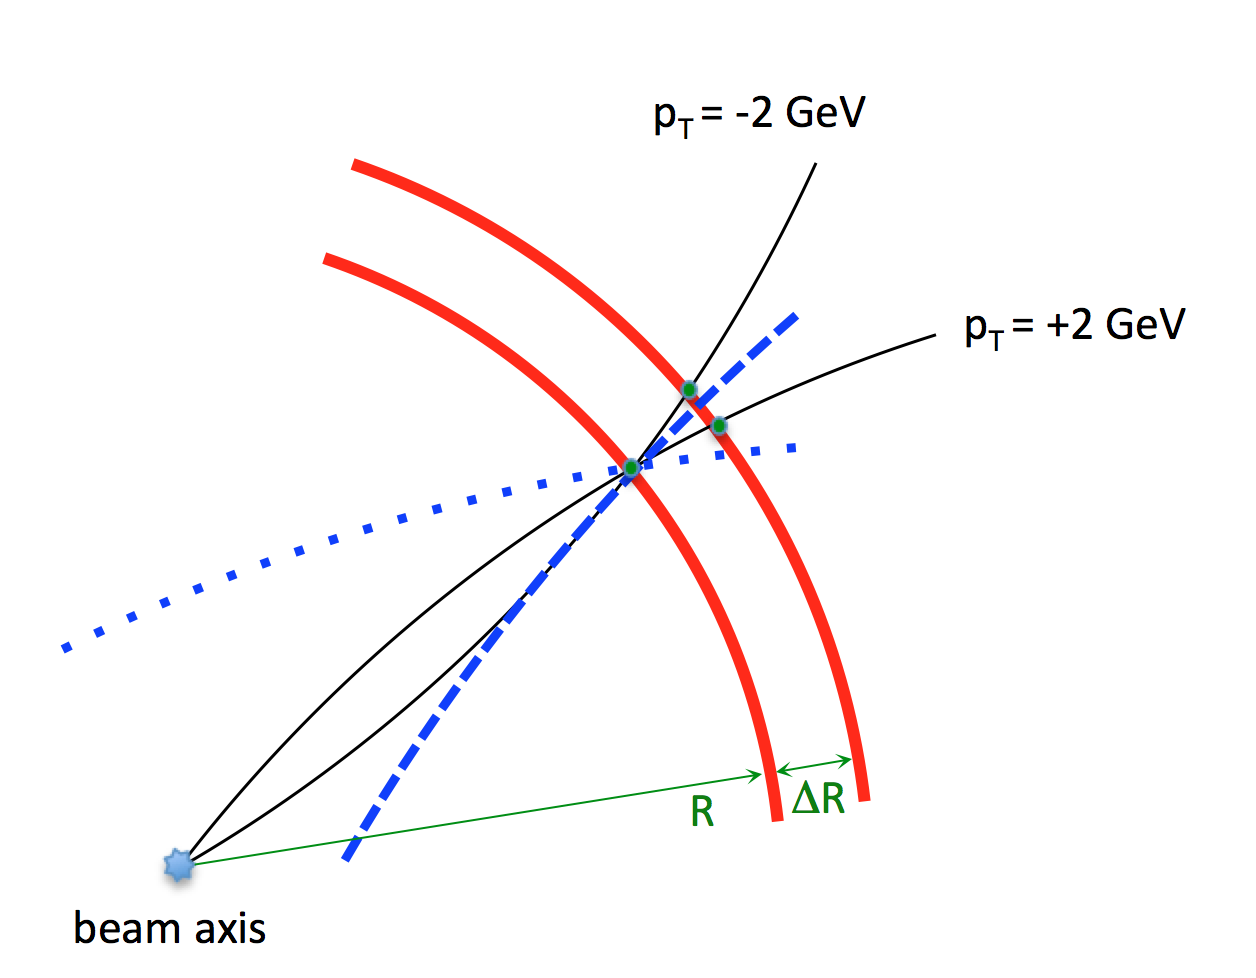
\includegraphics[width=0.47\textwidth]{figures/L1TT/geom.png}
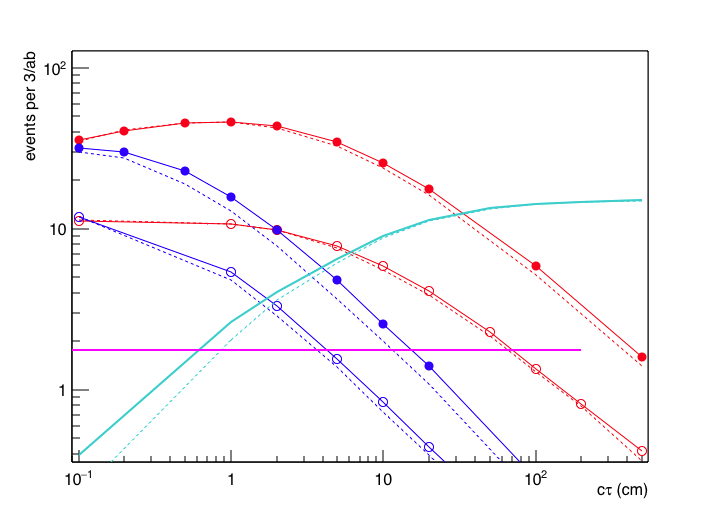
\includegraphics[width=0.47\textwidth]{figures/L1TT/final_h125.png}
\caption{ Left: Sketch of the toy stub formation in a doublet layer. Four tracks are passing through the same point in the inner layer.
Only the tracks hitting the outer layer between the two green points would produce a L1 stub. The dashed track does, and the dotted does not.
Right: Event yields for $Br[h\rightarrow\phi\phi\rightarrow 4q]=10^{-5}$ as a function of 
$\phi$ proper lifetime. Red curves correspond to
quad loose track jet trigger, blue - to quad tight track jet trigger. 
Open circles indicate track jets with $p_T$ above 20 GeV, filled circles - displaced track jets above 10 GeV. 
Teal curve corresponds to the  no-track 70 GeV di-jet trigger.
Purple line shows the expected yield from $Wh$ production triggered by a lepton from $W$.
}
\label{fig:tracktrigger_toy}
\end{center}
\end{figure}

The rare SM Higgs decays considered above is challenging, because of the small total $H_T$ in the event. 
While Higgs-like signals may be accessible in associated production, some new physics signals may not, such as dark matter models where the mass splitting between $chi_1$ and $chi_2$ is small. 
Those will benefit a lot from the displaced track trigger.

\subsection{New Ideas for Future Studies} \label{sec:upgradeideas}

\textbf{TBA}: coordinate with ATLAS \& theory

\subsubsection{New studies for HL-LHC} 

\begin{itemize}
\item \textbf{Inelastic dark matter} with displaced muon pairs: L1 track trigger; MTD
\item \textbf{Inelastic dark matter} with displaced photons: ECAL/HGCAL
\item \textbf{Dark showers}: L1 track trigger, MTD(?)
\end{itemize}

\subsubsection{New detectors at future collider}

\begin{itemize}
\item \textbf{4D pixel detector with timing} 
\item \textbf{Curtin, Zurita, et al, crazy tracker idea}: new tracking layer very close to beamline?
\end{itemize}
